\section*{Proof development of the common kernel}
\addcontentsline{toc}{section}{Proof development of the common kernel}

The following constructions develop the emission rules, the calendar with
memory, compatible sequences, cubic completion, regional readouts and the
reversibility of the dodecaphasic register. Their definitions and proofs precede
the arithmetic and spectral applications that use them. Fragments from Article I
retain their statements, proofs and source locators; the source manifest records
the corresponding components, line intervals and hashes.

References to alpha and the exceptional corridor specify the provenance of the
objects. Subsequent identifications with codes and lattices do not enter the
spectral proofs of this manuscript. References to Article I document that
provenance, while the necessary arguments are presented here in full. Finite
censuses and reconstructions retain the rules, domains and starting coordinates
of each statement; their inclusion does not alter the scope of global positivity
stated in the abstract.

% BEGIN NUCLEO_ADITIVO_20260921_CENSO
\clearpage
\section{Topological Phase Kernel and generation of the seed catalogue}
\label{act21:tpk:capitulo}

The two APP evaluations acquire generative efficacy once their activation,
evaluation position, positional transport and the information preserved by
each transition have been specified. The \emph{Topological Phase Kernel},
abbreviated TPK, combines these operations into a dynamics on enriched
states. Its definition comprises selection, transport, arithmetic updating
and preservation of the record. The finite construction developed in this
section provides the seeds on which the regional lifts and coinductive
prolongation subsequently act.

The principal result of this stage is a generated and classified catalogue:
the initial conditions of the two cursors produce integer emissions;
their ternary reading determines oriented words; and the dihedral action
organises these words into orbits. Each step preserves its preimages and
the relations that permit recovery of the preceding description. The chain
of cardinalities
\[
 104\,976\longrightarrow468\longrightarrow243\subset729,
 \qquad 243\longrightarrow43,
\]
abbreviates distinct objects. Each object is constructed and each count
justified below, before any of them is used as data for regional selection.

\subsection{Phase selection, transport and enriched state}
\label{act21:tpk:operaciones}

\subsubsection{Tritic selector of operative phase}

The nonadic phase takes its values in \(D_9=\{1,\ldots,9\}\). The tritic
selector is the function
\begin{equation}
 M_{\mathrm{ph}}:D_9\longrightarrow\{-1,0,+1\},\qquad
 M_{\mathrm{ph}}(g)=
 \begin{cases}
 +1,&g\in\{1,4,7\},\\
 -1,&g\in\{2,5,8\},\\
 0,&g\in\{3,6,9\}.
 \end{cases}
 \label{act21:tpk:selector}
\end{equation}
In the emitter realisation, the value \(+1\) activates the additive
evaluation, \(-1\) activates the multiplicative evaluation, and \(0\)
records the neutral event. The cardinal orientation of the cursor is
another state coordinate. This distinction specifies both the operation
being read and the direction in which its evaluation point is transported.

For transitions indexed by \(t\geq1\), the phase preceding the reading is
\begin{equation}
 g_t=1+[(t-1)]_9,\qquad \epsilon_t=M_{\mathrm{ph}}(g_t),
 \label{act21:tpk:fase}
\end{equation}
where \([n]_b\) denotes the representative of \(n\) modulo \(b\) in
\(\{0,\ldots,b-1\}\). A window of nine transitions contains the sequence
\((+1,-1,0,+1,-1,0,+1,-1,0)\).

\subsubsection{Oriented cursors and cardinal transport}

The indices \(I_9=\{0,\ldots,8\}\) are used for positions, and the positive
labels \((a,b)=(i+1,j+1)\) for APP evaluations. A finite cursor is
\[
 c=(i,j;d)\in\mathcal S:=I_9^2\times\mathcal D,
 \qquad \mathcal D=\{N,E,S,O\}.
\]
The four directions act by
\[
 v_N=(-1,0),\quad v_E=(0,1),\quad
 v_S=(1,0),\quad v_O=(0,-1).
\]
The cardinal map corresponding to \(d\) is
\[
 T_d(i,j)=\bigl([i+(v_d)_1]_9,[j+(v_d)_2]_9\bigr).
\]
Thus \(M_{\mathrm{ph}}\) and \(T_d\) have distinct domains, codomains
and actions. Tritic activation selects one of the two cursors; cardinal
transport changes its position in the direction already retained by that
cursor.

The integer lift of the cursor is
\(\widetilde c=(x,y;d)\in\mathbb Z^2\times\mathcal D\), with finite position
\(([x]_9,[y]_9)\). Its winding counts are recovered from
\begin{equation}
 x=9\lfloor x/9\rfloor+[x]_9,\qquad
 y=9\lfloor y/9\rfloor+[y]_9.
 \label{act21:tpk:vueltas}
\end{equation}
These two divisions concern spatial transport. The division of an additive
or multiplicative evaluation constitutes a distinct arithmetic record,
which is preserved together with them.

\subsubsection{Composition of the transition}

The state of the finite realisation includes the two lifted cursors, their
directions, the phase, the accumulators of the active window, the ordered
list of blocks already emitted and the transition record. Each local
record contains the preceding positions, the integer evaluations of both
sheets, their residues and quotients, the active regime and the
orientations. Prefix and boundary fields arising in a prolongation are
incorporated into the same state with their compatibility rules.

The transition is ordered as
\begin{equation}
 \mathcal U_t=\mathsf{Mem}_t\circ\mathsf{Tra}_t\circ\mathsf{Sel}_t.
 \label{act21:tpk:composicion}
\end{equation}
Selection determines the regime and preserves the sample taken before any
displacement. Transport applies the active movement and the cardinal
reversal prescribed by the schedule. Updating incorporates that sample
into the accumulators and the record; at the end of a window, it emits
the corresponding block. The composition therefore uses a sample taken
before transport, although its definitive storage occurs at the end of
the transition.

\subsection{Initial conditions and reversible enumeration}
\label{act21:tpk:semillas}

The additive and multiplicative sheets have independent cursors. The
domain of initial conditions is the ordered product
\[
 \Omega_{\mathrm{seed}}=\mathcal S_+\times\mathcal S_\times,
 \qquad |\mathcal S|=9^2\cdot4=324.
\]
Consequently,
\begin{equation}
 |\Omega_{\mathrm{seed}}|=324^2=104\,976.
 \label{act21:tpk:censo-inicial}
\end{equation}
The number \(81\) counts positions; \(324\) counts the oriented positions
of one cursor; \(104\,976\) counts ordered pairs of cursors. Choosing a
position in APP retains only part of an initial condition of the emitter.

Fix the numbering
\[
 \operatorname{ind}(N)=0,\quad\operatorname{ind}(E)=1,\quad
 \operatorname{ind}(S)=2,\quad\operatorname{ind}(O)=3,
\]
and define
\begin{equation}
 \nu(i,j;d)=4(9i+j)+\operatorname{ind}(d).
 \label{act21:tpk:indice-semilla}
\end{equation}

\begin{proposition}[Exact enumeration of the initial conditions]
\label{act21:tpk:enumeracion}
The map \(\nu\) is a bijection from \(\mathcal S\) onto
\(\{0,\ldots,323\}\). The pair of indices is reversibly encoded by
\(324\nu_++\nu_\times\in\{0,\ldots,104\,975\}\).
\end{proposition}
\begin{proof}
Division by four recovers
\[
 \operatorname{ind}(d)=[\nu]_4,\qquad
 j=[\lfloor\nu/4\rfloor]_9,\qquad i=\lfloor\nu/36\rfloor.
\]
The bounds on the domain ensure that these three quantities belong to
their respective index sets and reconstruct \(\nu\) through
\eqref{act21:tpk:indice-semilla}. For the pair, Euclidean division by \(324\)
recovers the quotient \(\nu_+\) and the residue \(\nu_\times\).
\end{proof}

The enumeration traverses the complete domain before any regional
grouping. The indices locate the preimages of an emission while keeping
explicit the condition that produced each trajectory.

\subsection{Sheet evaluation and arithmetic record}
\label{act21:tpk:lecturas}

At a positive position \((a,b)\), the integer evaluations are
\(A_+(a,b)=a+b\) and \(A_\times(a,b)=ab\). For \(n>0\), retain
\begin{equation}
 \rho_9(n)=1+[n-1]_9,\qquad
 q_9(n)=\lfloor(n-1)/9\rfloor,\qquad
 n=\rho_9(n)+9q_9(n).
 \label{act21:tpk:division-evaluacion}
\end{equation}
Additive activation incorporates \(\rho_9(A_+)\) into the corresponding
accumulator. Multiplicative activation uses an observable of the residue
\(\rho_9(A_\times)\), defined next.

\subsubsection{Discrete exponent in the units modulo nine}

The powers of \(2\) modulo \(9\) traverse
\[
 2^0,2^1,\ldots,2^5\equiv1,2,4,8,7,5\pmod9,
 \qquad 2^6\equiv1\pmod9.
\]
The discrete logarithm in this group of six units is represented by
\begin{equation}
 \ell_9(1)=0,\quad\ell_9(2)=1,\quad\ell_9(4)=2,
 \quad\ell_9(8)=3,\quad\ell_9(7)=4,\quad\ell_9(5)=5.
 \label{act21:tpk:logaritmo}
\end{equation}
The emission law extends the observable by
\(\ell_9(3)=\ell_9(6)=\ell_9(9)=0\). To preserve its provenance, the
recorded sample includes the original residue and the indicator of
membership in the group of units. An observed value of zero can therefore
originate from the unit \(1\) or from one of the three non-invertible
residues, with its origin remaining recoverable.

\subsubsection{Order of reading and movement}

Evaluations are performed at the positions preceding the transition.
If \(\epsilon_t=+1\), the additive reading is accumulated and its cursor
is displaced. If \(\epsilon_t=-1\), the multiplicative discrete exponent
is accumulated and the second cursor is displaced. If \(\epsilon_t=0\),
the neutral counter is incremented and both positions are preserved.

At the end of steps \(27\) and \(54\), both directions are replaced by
their opposites. The windows are concatenated with positions and
orientations preserved. At the start of each window, only its three local
accumulators are reset to zero; the preceding record remains available.

\begin{proposition}[Inversion of the lifted transport]
\label{act21:tpk:inversion}
Let \(a,b\in\{0,1\}\) be the activation and reversal indicators of a
cursor. If \(\operatorname{opp}\) interchanges \(N\leftrightarrow S\)
and \(E\leftrightarrow O\), the transformation
\[
 F_{a,b}(z,d)=\bigl(z+a v_d,\operatorname{opp}^{\,b}(d)\bigr)
\]
has inverse
\[
 F_{a,b}^{-1}(z',d')=
 \bigl(z'-a v_{\operatorname{opp}^{\,b}(d')},
       \operatorname{opp}^{\,b}(d')\bigr).
\]
Spatial reduction modulo nine intertwines this transformation with the
finite transport.
\end{proposition}
\begin{proof}
Applying opposition twice recovers the initial direction. Once that
direction has been recovered, subtracting \(a v_d\) reverses the
displacement. For the spatial projection, it suffices to use
\([z+a v_d]_9=[[z]_9+a v_d]_9\) componentwise. Directional reversal
preserves this equality.
\end{proof}

The phase determines the indicators used by the inverse. The spatial and
arithmetic records can therefore be preserved jointly, including when
the boundary of the representative \(I_9^2\) is crossed.

\subsection{Six windows and decimal block emission}
\label{act21:tpk:emision}

\subsubsection{Accumulation within a nonadic window}

Window \(m\), with \(1\leq m\leq6\), comprises steps
\(9m-8,\ldots,9m\). Let \(S_m\) be the sum of its active positive
additive residues, \(E_m\) the sum of its active discrete exponents, and
\(Z_m\) its number of neutral events.

\begin{lemma}[Activation multiplicities]
\label{act21:tpk:tres-eventos}
Each window contains three additive activations, three multiplicative
activations and three neutral activations. In particular, \(Z_m=3\).
\end{lemma}
\begin{proof}
The phases of a window traverse exactly \(1,\ldots,9\). Each of the
three sets in \eqref{act21:tpk:selector} has cardinality three.
\end{proof}

The six windows comprise \(54\) transitions and produce six blocks.
This length belongs to the initial emitter defined here. Continuation
in depth subsequently acts on the words and their compatible records.

\subsubsection{Decimal encoding rule}

The emission law specifies the digits
\begin{align}
 d_{m,1}&=[S_m]_{10},\notag\\
 d_{m,2}&=[S_m+E_m]_{10},\notag\\
 d_{m,3}&=[3S_m+5E_m+7Z_m]_{10},\notag\\
 U_m&=100d_{m,1}+10d_{m,2}+d_{m,3}.
 \label{act21:tpk:bloque-decimal}
\end{align}
The weights \(100,10,1\) are the hundreds, tens and units positions.
The subscript \(10\) denotes the decimal residue, and each block satisfies
\(0\leq U_m\leq999\). The emitted word is the ordered sequence
\(\mathbf U=(U_1,\ldots,U_6)\), with a fixed width of three digits per
block.

The coefficients \(3,5,7\) constitute the explicit weights of this
emission law. Once the rule has been fixed, each digit is calculated from
the accumulators, and the results of this section follow from that rule.
The number \(1\) appearing in its reduced form has a further specific
provenance: \(7Z_m=21\equiv1\pmod{10}\).

If \(s_m=[S_m]_{10}\) and \(e_m=[E_m]_{10}\), one obtains
\begin{equation}
 G(s_m,e_m)=100s_m+10[s_m+e_m]_{10}
                   +[3s_m+5e_m+1]_{10}=U_m.
 \label{act21:tpk:acoplamiento-firmas}
\end{equation}
Here the letter \(e_m\) denotes a component of the discrete-exponent
signature. Its definition belongs to the finite emitter.

\begin{proposition}[Recovery of the two signatures]
\label{act21:tpk:recuperacion-firmas}
The map \(G:\{0,\ldots,9\}^2\to\{0,\ldots,999\}\) is injective.
For a block \(U=100a+10b+c\) in its image, the inverse is
\[
 s=a,\qquad e=[b-a]_{10},\qquad
 c=[3s+5e+1]_{10}.
\]
Consequently, the word \(\mathbf U\) determines the two six-component
signatures \(\mathbf s\) and \(\mathbf e\).
\end{proposition}
\begin{proof}
The last two summands of \eqref{act21:tpk:acoplamiento-firmas} belong to
\(\{0,\ldots,99\}\), so the hundreds digit recovers \(s\). The tens digit
is \([s+e]_{10}\); subtracting \(s\) and reducing modulo ten recovers
\(e\). The units digit verifies the third congruence. The reconstruction
applies independently to the six positions of the word.
\end{proof}

The integer totals \(S_m,E_m\) are recovered from the recorded readings;
the hundreds and tens digits recover their residues. For example, a total
\(S_m=15\) produces \(s_m=5\). This distinction identifies precisely
which information each level of encoding preserves.

\subsubsection{Positional encoding of the six-block word}

The six blocks admit a fixed-width integer encoding,
\begin{equation}
 \mathscr N(\mathbf U)=\sum_{m=1}^{6}U_m1000^{6-m},
 \qquad0\leq\mathscr N(\mathbf U)<1000^6.
 \label{act21:tpk:entero-base1000}
\end{equation}
The first block occupies the position of greatest weight, and the sixth
the base-thousand units position. A block \(058\) occupies a complete
position with integer value \(58\); its three-digit width belongs to
the decimal presentation of that position.

\begin{proposition}[Positional recovery of the emissions]
\label{act21:tpk:inversa-base1000}
The encoding \eqref{act21:tpk:entero-base1000} determines the complete word by
\[
 U_m=\left[\left\lfloor
 \frac{\mathscr N(\mathbf U)}{1000^{6-m}}\right\rfloor\right]_{1000},
 \qquad1\leq m\leq6.
\]
\end{proposition}
\begin{proof}
On division by \(1000^{6-m}\), the preceding blocks yield integer
multiples of \(1000\), block \(m\) yields \(U_m\), and the contribution
of the subsequent blocks belongs to \([0,1)\). Taking the integer part
eliminates the latter contribution, and the residue modulo \(1000\)
eliminates the former.
\end{proof}

This encoding preserves the six emissions. Its domain has ordered
base-thousand positions, whereas the APP domain has spatial positions
modulo nine. The composition retains both indices: \(m\) identifies an
emission window, and \((i,j)\) identifies the cell visited during a
transition in that window.

\subsection{Complete calculation of an emission beginning with 501}
\label{act21:tpk:ejemplo501}

Fix the initial conditions
\[
 c_{+,0}=(0,4;N),\qquad c_{\times,0}=(2,3;N),
 \qquad \nu_+=16,\quad\nu_\times=84.
\]
The initial positive positions are \((1,5)\) and \((3,4)\). The preceding
chronological index is \(t=0\), the first phase read is \(g_1=1\), and
the record is empty. These coordinates are the inputs to the calculation;
the blocks are obtained by executing the recurrence.

\begin{table}[htbp]
\caption{First window: preceding readings and active accumulation.}
\label{act21:tpk:tabla-501}
\small
\begin{tabular}{@{}rcccrrr@{}}
\toprule
\(t\)&\(\epsilon_t\)&position \(+\)&position \(\times\)&
\(\Delta S\)&\(\Delta E\)&\((S,E,Z)\)\\
\midrule
1&\(+1\)&\((1,5)\)&\((3,4)\)&6&0&\((6,0,0)\)\\
2&\(-1\)&\((9,5)\)&\((3,4)\)&0&0&\((6,0,0)\)\\
3&0&\((9,5)\)&\((2,4)\)&0&0&\((6,0,1)\)\\
4&\(+1\)&\((9,5)\)&\((2,4)\)&5&0&\((11,0,1)\)\\
5&\(-1\)&\((8,5)\)&\((2,4)\)&0&3&\((11,3,1)\)\\
6&0&\((8,5)\)&\((1,4)\)&0&0&\((11,3,2)\)\\
7&\(+1\)&\((8,5)\)&\((1,4)\)&4&0&\((15,3,2)\)\\
8&\(-1\)&\((7,5)\)&\((1,4)\)&0&2&\((15,5,2)\)\\
9&0&\((7,5)\)&\((9,4)\)&0&0&\((15,5,3)\)\\
\bottomrule
\end{tabular}
\par\smallskip\noindent{\footnotesize\emph{Note.} Positions are positive
labels of the cells preceding movement. Neutral events increment only \(Z\).}
\end{table}

The three active additive evaluations are
\[
 1+5=6,\qquad9+5=14=5+9,\qquad8+5=13=4+9,
\]
so \(S_1=6+5+4=15\). The three active multiplicative evaluations are
\(3\cdot4=12\), \(2\cdot4=8\) and \(1\cdot4=4\). Their positive
residues are \(3,8,4\), with observables \(0,3,2\); hence \(E_1=5\).
Finally, \(Z_1=3\). The decimal rule gives
\[
 d_{1,1}=[15]_{10}=5,\quad
 d_{1,2}=[15+5]_{10}=0,\quad
 d_{1,3}=[45+25+21]_{10}=1,
\]
and one obtains \(U_1=501\).

The second additive reading above has arithmetic quotient \(1\), whereas
its lifted cursor is at \((-1,4;N)\), with vertical winding count \(-1\).
These are distinct data in the same record. Both participate in the
complete recovery of the evaluation and its position.

\begin{table}[htbp]
\caption{The six windows of initial condition \((16,84)\).}
\label{act21:tpk:tabla-seis501}
\begin{tabular}{@{}rrrrrrrr@{}}
\toprule
\(m\)&steps&\(S_m\)&\(E_m\)&\(Z_m\)&\(s_m\)&\(U_m\)&\([-U_m]_3\)\\
\midrule
1&1--9&15&5&3&5&501&0\\
2&10--18&6&5&3&6&614&1\\
3&19--27&24&5&3&4&498&0\\
4&28--36&21&5&3&1&169&2\\
5&37--45&12&5&3&2&272&1\\
6&46--54&12&5&3&2&272&1\\
\bottomrule
\end{tabular}
\end{table}

The resulting word and its signatures are
\begin{align*}
 \mathbf U&=(501,614,498,169,272,272),\\
 \mathbf s&=(5,6,4,1,2,2),&
 \mathbf e&=(5,5,5,5,5,5).
\end{align*}
Cardinal reversal after step \(27\) changes the trajectories of the final
three windows. The repeated block \(272\) corresponds to two successive
windows with their own positions and chronological record.

As a second case, the minimal initial condition
\((\nu_+,\nu_\times)=(0,0)\) produces
\[
 \mathbf U=(252,109,252,903,850,850),\quad
 \mathbf s=(2,1,2,9,8,8),\quad
 \mathbf e=(3,9,3,1,7,7).
\]
In this case, both cursors return to their initial positions and
orientations after \(54\) transitions. The nonadic phase completes six
cycles, the chronological counter advances by \(54\) units, and the
record contains \(54\) samples. The positional reading of the return and
the recorded history describe distinct properties of the execution.

\subsection{Factorisation of the finite census}
\label{act21:tpk:censo}

The signatures \(f_+(\nu)=\mathbf s\) and
\(f_\times(\nu)=\mathbf e\) are calculated by executing the corresponding
cursor through the six windows. The independence of positions and
directions between the two cursors gives
\begin{equation}
 T_{\mathrm{em}}(\nu_+,\nu_\times)
   =G^{(6)}\bigl(f_+(\nu_+),f_\times(\nu_\times)\bigr),
 \label{act21:tpk:factorizacion}
\end{equation}
where \(G^{(6)}\) applies \eqref{act21:tpk:acoplamiento-firmas} at each position.
This factorisation first permits enumeration of \(324+324\) trajectories
and then combination of the distinct signatures, preserving the
multiplicities of their preimages.

\par\noindent\begin{minipage}{\linewidth}
\subsubsection{Images of the two signatures}

The following tables include every signature. Its multiplicity is the
number of initial conditions producing it; the minimal index locates one
such condition. The complete preimage is defined by
\[
 f_\sigma^{-1}(a)=\{\nu\in\{0,\ldots,323\}:f_\sigma(\nu)=a\}.
\]
The recurrence of the preceding sections determines every element of
this set by a finite integer calculation.

\begin{table}[H]
\centering\fontsize{9.5}{11.4}\selectfont
\setlength{\abovecaptionskip}{8pt}\setlength{\belowcaptionskip}{6pt}
\renewcommand{\arraystretch}{1.12}
\caption{The eighteen additive signatures.}
\label{act21:tpk:firmas-aditivas}
\begin{tabular}{@{}lrr@{\qquad}lrr@{}}
\toprule
signature&multiplicity&\(\nu_{\min}\)&signature&multiplicity&\(\nu_{\min}\)\\
\midrule
\texttt{122564}&18&17&\texttt{564122}&18&16\\
\texttt{122898}&18&24&\texttt{645212}&18&4\\
\texttt{212645}&18&5&\texttt{654889}&18&33\\
\texttt{212988}&18&0&\texttt{889221}&18&13\\
\texttt{221456}&18&29&\texttt{889654}&18&32\\
\texttt{221889}&18&12&\texttt{898122}&18&25\\
\texttt{456221}&18&28&\texttt{898465}&18&20\\
\texttt{465898}&18&21&\texttt{988212}&18&1\\
\texttt{546988}&18&9&\texttt{988546}&18&8\\
\bottomrule
\end{tabular}

\par\vspace{12pt}

\caption{The twenty-six multiplicative signatures.}
\label{act21:tpk:firmas-multiplicativas}
\begin{tabular}{@{}lrr@{\qquad}lrr@{}}
\toprule
signature&multiplicity&\(\nu_{\min}\)&signature&multiplicity&\(\nu_{\min}\)\\
\midrule
\texttt{000000}&108&8&\texttt{555555}&24&84\\
\texttt{177393}&8&1&\texttt{555717}&8&14\\
\texttt{177555}&8&54&\texttt{555771}&8&18\\
\texttt{177771}&8&11&\texttt{555933}&8&24\\
\texttt{339555}&8&6&\texttt{717555}&8&12\\
\texttt{339771}&8&15&\texttt{717717}&8&21\\
\texttt{339933}&8&59&\texttt{717933}&8&19\\
\texttt{393177}&8&0&\texttt{771177}&8&9\\
\texttt{393393}&8&45&\texttt{771339}&8&13\\
\texttt{393555}&8&40&\texttt{771555}&8&16\\
\texttt{555177}&8&52&\texttt{933339}&8&57\\
\texttt{555339}&8&4&\texttt{933555}&8&26\\
\texttt{555393}&8&41&\texttt{933717}&8&17\\
\bottomrule
\end{tabular}
\end{table}
\end{minipage}\par


\begin{proposition}[Image and multiplicities of the emitter]
\label{act21:tpk:468}
The image \(\mathcal U_6=\operatorname{im}T_{\mathrm{em}}\) contains
\(468\) distinct words. Their preimages are distributed into \(432\)
fibres of cardinality \(144\), \(18\) of cardinality \(432\) and \(18\)
of cardinality \(1944\).
\end{proposition}
\begin{proof}
Exhaustive evaluation of the algorithm in Section~\ref{act21:tpk:algoritmo}
on the indices \(0,\ldots,323\) gives the two tables above.
The first partition has \(18\) classes of cardinality \(18\); the second
has \(24\) classes of cardinality \(8\), one of cardinality \(24\) and
one of cardinality \(108\). The sums \(18\cdot18=324\) and
\(24\cdot8+24+108=324\) verify the total mass of both partitions.
Proposition~\ref{act21:tpk:recuperacion-firmas} makes the coupling of their
images injective; there are therefore \(18\cdot26=468\) emissions.
By \eqref{act21:tpk:factorizacion}, the preimage of a pair of signatures is
the product of their two preimages. This gives \(18\cdot24=432\)
products of cardinality \(18\cdot8=144\), \(18\) of cardinality
\(18\cdot24=432\), and \(18\) of cardinality \(18\cdot108=1944\).
Finally,
\[
 432\cdot144+18\cdot432+18\cdot1944=104\,976.
\]
The enumerative part is an exact finite check of the recurrence; the
factorisation explains why this count covers every pair.
\end{proof}

The emission in Example~\ref{act21:tpk:ejemplo501} has a fibre of cardinality
\(18\cdot24=432\). The example with indices \((0,0)\) has a fibre of
cardinality \(18\cdot8=144\). In both cases, the emitted word recovers
the signatures, whereas identification of a particular initial condition
uses its index or its trajectory record.

\subsection{Oriented ternary reading and preservation of fibres}
\label{act21:tpk:reduccion-ternaria}

Oriented reduction acts separately on each block:
\begin{equation}
 \Psi:\mathcal U_6\longrightarrow\mathbb F_3^6,\qquad
 \Psi(U_1,\ldots,U_6)=([-U_1]_3,\ldots,[-U_6]_3).
 \label{act21:tpk:psi}
\end{equation}
Its sign fixes an orientation of the catalogue. The balanced identification
\(0\mapsto0\), \(1\mapsto+1\), \(2\mapsto-1\) is then applied
componentwise.

Modulo nine organises APP evaluations and positions; residues modulo ten
form each digit; base thousand combines three decimal positions; and
modulo three determines the ternary signature of each block. These four
uses have defined objects and functions. In particular, \(\Psi\) reads
six blocks and produces six trits; a positional conversion of the integer
formed by eighteen digits would be a different operation.

For the two conditions already calculated, one obtains
\begin{align*}
 \Psi(501,614,498,169,272,272)&=(0,1,0,2,1,1),\\
 \Psi(252,109,252,903,850,850)&=(0,2,0,0,2,2).
\end{align*}
The decimal emitter is defined before this reduction. The function of
\(\Psi\) is to produce the ternary object on which orbital symmetry and
regional selectors act. This function explains its position in the
genealogy: it connects an already calculated emission with a structural
classification.

The image \(\mathcal W_6:=\Psi(\mathcal U_6)\) contains exactly \(243\)
words within the ambient set of \(3^6=729\) words. Enumeration by the
final algorithm gives the histogram
\begin{equation}
\begin{array}{c|rrrrrr}
 |\Psi^{-1}(w)|&1&2&3&4&5&6\\\hline
 \text{number of words }w&132&66&18&3&6&18.
\end{array}
\label{act21:tpk:fibras-ternarias}
\end{equation}
The sums for the two readings are
\[
132+66+18+3+6+18=243,
\qquad132+2\cdot66+3\cdot18+4\cdot3+5\cdot6+6\cdot18=468.
\]
The first counts ternary words; the second recovers the number of
emissions distributed among their fibres.

\begin{example}[Two emissions with the same ternary signature]
\label{act21:tpk:colision}
The emissions
\[
 (498,501,614,252,252,109),\qquad
 (870,810,923,252,252,109)
\]
are distinct and both have image \((0,0,1,0,0,2)\) under \(\Psi\).
Each has \(144\) initial conditions. The ternary word preserves a reading
class; the emissions and their preimages distinguish the data that
converge in that class.
\end{example}

Preservation of fibres is expressed concretely by
\[
 \mathcal F_w=\{\mathbf U\in\mathcal U_6:\Psi(\mathbf U)=w\},
 \qquad
 \Omega_{\mathbf U}=T_{\mathrm{em}}^{-1}(\mathbf U).
\]
The complete preimage of \(w\) in the initial domain is therefore the
disjoint union of the sets \(\Omega_{\mathbf U}\), with
\(\mathbf U\in\mathcal F_w\). The enriched record can retain the
emission, its signatures and the initial condition together with its
ternary reading. The exact inverse then concerns the recorded datum with
its type; the isolated six-trit word retains the precise scope of
\eqref{act21:tpk:psi}.

\subsection{Dihedral action and the forty-three orbits}
\label{act21:tpk:orbitas}

Define the following permutations on six coordinates:
\begin{align}
 r(u_1,u_2,u_3,u_4,u_5,u_6)
   &=(u_3,u_1,u_2,u_5,u_6,u_4),\\
 s(u_1,u_2,u_3,u_4,u_5,u_6)
   &=(u_4,u_5,u_6,u_1,u_2,u_3).
 \label{act21:tpk:generadores-diedrales}
\end{align}
The first rotates the two groups of three coordinates in conjugate
directions; the second interchanges the groups. Their composition
satisfies \(r^3=s^2=1\) and \(srs=r^{-1}\). They therefore generate an
action of the six-element dihedral group \(D_3\).

\begin{proposition}[Equivariance and stability of the catalogue]
\label{act21:tpk:equivarianza}
Reduction by \(\Psi\) commutes with the action of \(D_3\). The sets
\(\mathcal U_6\) and \(\mathcal W_6\) are stable under its generators.
\end{proposition}
\begin{proof}
The equality \(\Psi(g\mathbf U)=g\Psi(\mathbf U)\) holds at every
coordinate because \(g\) permutes positions and \(\Psi\) applies the
same reduction at each position. Stability of the catalogue is a further
check: generating its \(468\) elements by
\eqref{act21:tpk:factorizacion}, one verifies that \(r\mathbf U\) and
\(s\mathbf U\) again belong to that set. The algorithm in
Section~\ref{act21:tpk:algoritmo} performs these membership checks.
Equivariance then transfers stability to the ternary image.
\end{proof}

\begin{proposition}[Complete orbital decomposition]
\label{act21:tpk:43}
The set \(\mathcal W_6\) decomposes into \(43\) orbits: \(38\) of
cardinality six and \(5\) of cardinality three.
\end{proposition}
\begin{proof}
For each \(w\in\mathcal W_6\), form
\[
 \mathcal O(w)=\{w,rw,r^2w,sw,srw,sr^2w\}.
\]
Choose the lexicographically least word in this set as representative.
Two words have the same representative exactly when they belong to the
same orbit. The algorithm generates the list of representatives in
Table~\ref{act21:tpk:representantes}; their cardinalities sum to
\(38\cdot6+5\cdot3=243\). Since every word in the catalogue participates
in this operation and the catalogue is stable, the list covers the
entire image.
\end{proof}

\begin{table}[htbp]
\caption{Minimal representatives and cardinalities of the forty-three orbits.}
\label{act21:tpk:representantes}
\small
\begin{tabular}{@{}lr@{\qquad}lr@{\qquad}lr@{}}
\toprule
representative&cardinality&representative&cardinality&representative&cardinality\\
\midrule
\texttt{001002}&6&\texttt{002112}&6&\texttt{012222}&6\\
\texttt{001011}&6&\texttt{002211}&6&\texttt{021022}&6\\
\texttt{001012}&6&\texttt{002220}&6&\texttt{021121}&6\\
\texttt{001021}&6&\texttt{011021}&6&\texttt{021202}&6\\
\texttt{001022}&6&\texttt{011112}&6&\texttt{022022}&3\\
\texttt{001100}&3&\texttt{011120}&6&\texttt{022112}&6\\
\texttt{001101}&6&\texttt{011201}&6&\texttt{022121}&6\\
\texttt{001110}&6&\texttt{011211}&6&\texttt{022202}&3\\
\texttt{001112}&6&\texttt{011220}&6&\texttt{022211}&6\\
\texttt{001202}&6&\texttt{011222}&6&\texttt{022222}&6\\
\texttt{001210}&6&\texttt{012112}&6&\texttt{112112}&3\\
\texttt{001211}&6&\texttt{012121}&6&\texttt{112211}&3\\
\texttt{001220}&6&\texttt{012202}&6&\texttt{112222}&6\\
\texttt{001222}&6&\texttt{012210}&6&&\\
\texttt{002012}&6&\texttt{012220}&6&&\\
\bottomrule
\end{tabular}
\end{table}

The orbits inherit integer invariants from their fibres. For each word,
\(n(w)=|\mathcal F_w|\) counts emissions, whereas
\[
 M(w)=\sum_{\mathbf U\in\mathcal F_w}|\Omega_{\mathbf U}|
\]
counts initial conditions. The symbol census \(c(w)=(n_0,n_1,n_2)\)
records the number of occurrences of each ternary class.
Together with the orientation and the support of the trajectories,
these data provide the predicates for subsequent regional selection.
The classification thus preserves more information than the form of a
representative word.

\subsection{Self-contained enumeration and verification algorithm}
\label{act21:tpk:algoritmo}

The enumeration uses integers, finite lists and the operations already
defined. The following procedure specifies its execution; \(\sigma\)
takes the values \(+\) and \(\times\).

\begin{enumerate}
\item For each \(\nu=0,\ldots,323\), recover \((i,j;d)\) using the
inverse of \eqref{act21:tpk:indice-semilla}. Initialise an empty signature list.
\item For each window \(m=1,\ldots,6\), initialise the accumulator
\(A=0\). Traverse \(t=9m-8,\ldots,9m\), calculating \(\epsilon_t\)
by \eqref{act21:tpk:fase}.
\item If \(\sigma=+\) and \(\epsilon_t=+1\), add
\(\rho_9(i+j+2)\) to \(A\) and update
\((i,j)\leftarrow T_d(i,j)\). If \(\sigma=\times\) and
\(\epsilon_t=-1\), add
\(\ell_9(\rho_9((i+1)(j+1)))\) and perform the same transport.
\item At the end of \(t=27\) or \(t=54\), replace \(d\) by its
opposite. At the end of the window, append \([A]_{10}\) to the
signature list. Preserve the position and direction for the next window.
\item Group the \(324\) indices according to equality of their
six-component lists. These two groupings give \(f_+\), \(f_\times\)
and all their preimages.
\item For each pair of distinct signatures, apply \(G^{(6)}\).
Assign to the emission the product multiplicity of the two preimages.
Verify signature recovery in each block and the sum of multiplicities
\(104\,976\).
\item Apply \(\Psi\) to each emission and group by equality of words.
Count the \(243\) values and the multiplicities in
\eqref{act21:tpk:fibras-ternarias}.
\item Apply \(r,s\) to each emission and verify membership in the
catalogue. For each ternary word, form its six dihedral images, remove
repetitions and record its lexicographic minimum. Count the \(43\)
orbits and the two sizes in Table~\ref{act21:tpk:representantes}.
\end{enumerate}

The execution terminates: the first stage evaluates \(648\) trajectories
of \(54\) transitions; the second combines \(468\) pairs of signatures;
the third groups a set of \(243\) words. An additional direct check can
execute the \(104\,976\) pairs and compare the result with the
factorisation \eqref{act21:tpk:factorizacion}; its scope is the same finite
domain.

\subsection{Preservation of the record and the function of the seeds}
\label{act21:tpk:conclusion}

Let \(\mathsf{Sample}(q_t)\) be the sample preceding the transition, and
\(\mathcal M_t\) the accumulated record. The memory update is
\begin{equation}
 \mathcal M_{t+1}=\mathcal M_t\mathbin{\Vert}\mathsf{Sample}(q_t),
 \label{act21:tpk:archivo}
\end{equation}
where \(\Vert\) denotes ordered concatenation. Induction gives
\[
 \mathcal M_n=\mathcal M_0\mathbin{\Vert}
 (\mathsf{Sample}(q_0),\ldots,\mathsf{Sample}(q_{n-1})).
\]
The accumulators are reconstructed by summing the active contributions
of each segment of nine records. Their quotients, the winding counts
of the cursors and the orientations remain associated with the same
transitions. Execution determines that record through the recurrence;
storage preserves the specific provenance of the readings.

At the end of this stage, the complete domain of initial conditions,
decimal emission, its two recoverable signatures, the ternary image,
its fibres and its orbital classification have been constructed.
The counts \(104\,976\), \(468\), \(243\), \(729\) and \(43\) now
have a domain and a mechanism of derivation. Regional selections receive
these structures with their invariants, and the lifts act on oriented
words with preserved provenance. This continuity makes the finite
catalogue a constructive antecedent of the coinductive development.

% END NUCLEO_ADITIVO_20260921_CENSO
% Fragmento conservado; véase MANIFIESTO_ANTECEDENTES_LECTURA.json.
\section{Development of the formal kernel: initial conditions, geometry, and refinement}
\label{sec:extension}

The support of eighty-one positions does not coincide with the domain of initial conditions of the dynamics. An initial condition must also specify an orientation; and the additive and multiplicative sheets have independent cursors. This distinction makes it possible to reconstruct the emission exhaustively without selecting a numerical region in advance.

\subsection{Initial states and the emission recurrence}

For enumeration we use indices \(I_9=\{0,\ldots,8\}\), related to the positive labels by \(i\mapsto i+1\). Let
\[
 \mathcal S=I_9^2\times\{N,E,S,O\},\qquad
 \Omega_{\rm seed}=\mathcal S_+\times\mathcal S_\times.
\]
Each initial condition \(\omega=(s_+,s_\times)\) determines two positions and two directions. The domain comprises all ordered pairs, so that
\begin{equation}
 |\mathcal S|=324,\qquad |\Omega_{\rm seed}|=324^2=104\,976.
 \label{eq:semillas}
\end{equation}
The independent annex enumerates all these conditions; the main text presents the law transforming them. The rows of an emission table are fibers of this domain of initial conditions.

The finite realization uses six windows of nine transitions. At each instant \(t\), the phase signature is \(M_{\rm ph}(1+((t-1)\bmod9))\). If it equals \(+1\), the positive residue \(\Sigma(i+1,j+1)=\rho_9(i+j+2)\) of the first cursor is read and that cursor is then moved; if it equals \(-1\), the positive residue \(\Pi(i+1,j+1)=\rho_9((i+1)(j+1))\) of the second cursor is read and the second cursor is then moved. A zero value increments the neutral counter. Upon completion of transitions twenty-seven and fifty-four, the cardinal orientations are reversed. The integer evaluations and their quotients are retained in the record, but the emitter uses the residual readouts specified here.

In the unit sector, the multiplicative readout uses the base-two discrete logarithm in \((\ZZ/9\ZZ)^\times\):
\[
 \ell_9(1)=0,\quad\ell_9(2)=1,\quad\ell_9(4)=2,\quad
 \ell_9(8)=3,\quad\ell_9(7)=4,\quad\ell_9(5)=5.
\]
For finite emission, it is extended with value zero to the nonunit sector. This extension is an observable, not an identification of the elements \(3,6,9\) with the multiplicative unit. The sheet and its membership in the radical sector remain in the trajectory record.

Let \(S_m\) be the sum of the three positive additive residues \(\Sigma\) of window \(m\), \(E_m\) the sum of the three discrete exponents of the multiplicative residues \(\Pi\), and \(Z_m=3\) the number of neutral events. Thus, \(S_m\) does not sum the integer evaluations \(S=i+j\), whose quotients remain in the record. With \([a]_{10}\in\{0,\ldots,9\}\), the decimal emission rule is
\begin{align}
 d_{m,1}&=[S_m]_{10},\notag\\
 d_{m,2}&=[S_m+E_m]_{10},\notag\\
 d_{m,3}&=[3S_m+5E_m+7Z_m]_{10},\notag\\
 U_m&=100d_{m,1}+10d_{m,2}+d_{m,3}.
 \label{eq:emisor-seis}
\end{align}
The integer coefficients and the calendar of this recurrence are an explicit part of the declared emission law. No values of \(\pi,\varphi,e\) or \(\alpha\) are received. The distinction between an emission rule and a constant recognized from its output prevents the genealogy from being hidden in a table of decimals.

If \(s_m=[S_m]_{10}\) and \(e_m=[E_m]_{10}\), the same rule is written as
\begin{equation}
 U_m=100s_m+10[s_m+e_m]_{10}+[3s_m+5e_m+1]_{10}.
 \label{eq:acoplamiento}
\end{equation}
The final one is the residue of \(7Z_m=21\) modulo ten. The oriented ternary reduction of the catalog adopts the convention
\begin{equation}
 \Psi(U_1,\ldots,U_6)=([-U_1]_3,\ldots,[-U_6]_3).
 \label{eq:psi-catalogo}
\end{equation}
The sign of this chart is explicit: changing it modifies the words and requires transporting the subsequent orientations. The balanced identification of each component of \(\FF_3\) with the TRIT is performed after \eqref{eq:psi-catalogo}.

\begin{proposition}[Injective factorization of the emission]
The word \(U=(U_1,\ldots,U_6)\) determines the two signatures \(s=(s_1,\ldots,s_6)\) and \(e=(e_1,\ldots,e_6)\). The emission image has \(18\cdot26=468\) elements. The ternary projection has \(243\) distinct values in the ambient space of \(729\) words.
\end{proposition}
\begin{proof}
The hundreds digits of \(U_m\) recover \(s_m\). If \(b_m\) is its tens digit, then \(e_m=[b_m-s_m]_{10}\). The units digit checks the third congruence of \eqref{eq:acoplamiento}. Hence the coupling is injective on the product of signatures.

Enumeration of the \(324\) conditions of one cursor through the preceding recurrence produces eighteen additive signatures, each with eighteen preimages; and twenty-six multiplicative signatures, of which twenty-four have eight preimages, one has twenty-four, and one has one hundred and eight. The annex preserves these signatures and their initial conditions, allowing the finite enumeration to be repeated without a reference numerical catalog. Injectivity of the coupling gives \(18\cdot26\) emissions and multiplicities
\[
 \underbrace{432}_{18\cdot24}\text{ fibers of }144,
 \qquad18\text{ fibers of }432,
 \qquad18\text{ fibers of }1944.
\]
The sum is \(432\cdot144+18\cdot432+18\cdot1944=104\,976\). Applying \eqref{eq:psi-catalogo} to the \(468\) emissions produces exactly \(243\) words. This last figure is the cardinality of the image, not that of the space \(\FF_3^6\).
\end{proof}

This factorization explains the difference between finite exhaustiveness and unbounded depth. The domain \eqref{eq:semillas} is complete for the declared support and emitter; it does not contain every prefix of every prolongation in advance. Depth belongs to the system of compatible extensions constructed over those conditions.

\subsection{Closure of the calendar and advancement of memory}

The calendar of one hundred and eight transitions consists of twelve nonadic windows. Its group structure is more precise than an informal product of two periods:
\begin{equation}
 0\longrightarrow C_{12}\xrightarrow{\iota}C_{108}
 \xrightarrow{p}C_9\longrightarrow0,
 \quad\iota([b])=[9b],\quad p([t])=[t]_9.
 \label{eq:extension108}
\end{equation}
If \(t=9b+r\) with \(0\le r<9\), the sum of two phases produces the carry
\[
 (b,r)+(b',r')=
 \left(b+b'+\left\lfloor\frac{r+r'}9\right\rfloor,\ [r+r']_9\right),
\]
where the first coordinate is reduced modulo twelve. Composition preserves the term linking the two coordinates.

\begin{proposition}[Nonsplitting of the calendar]
The sequence \eqref{eq:extension108} is exact and admits no section that is a group homomorphism.
\end{proposition}
\begin{proof}
The kernel of reduction modulo nine is the subgroup of multiples of nine, the image of \(\iota\). If the extension split, commutativity would give \(C_{108}\cong C_{12}\times C_9\). The first group has exponent \(108\), whereas the second has exponent \(\operatorname{mcm}(12,9)=36\), a contradiction.
\end{proof}

Nine transitions restore the nonadic phase and advance one window; one hundred and eight restore the finite calendar. Neither fact requires erasing the trajectory or restoring the prefix of a prolongation. The nonadic holonomy \(\Gamma_9\) denotes transport through one winding on states with memory, so that
\begin{equation}
 g(\Gamma_9x)=g(x),\qquad M(\Gamma_9x)=M(x)+1.
 \label{eq:holonomia-memoria}
\end{equation}
Phase equality and memory increment are compatible and constitute two observations of the same transport.


\subsection{Observable compression and orthogonal conservation}

An isometric realization allows what a reduced observation loses to be expressed quantitatively. Let \(U:\mathcal H\to\mathcal H\) be an isometric realization of transport through one winding, \(U^*U=I\), and \(J:\mathcal H_{\rm vis}\to\mathcal H\) an isometric inclusion. Define
\[
 T=J^*UJ,\qquad D=(I-JJ^*)UJ.
\]
Then
\begin{equation}
 UJ=JT+D,\qquad J^*D=0,\qquad I-T^*T=D^*D.
 \label{eq:conservacion-ortogonal}
\end{equation}
The last equality follows by taking the adjoint product of the first and using orthogonality. Contraction of the visible component does not by itself constitute destruction of information in the total state.

\begin{proposition}[Conservation over a finite horizon]
If \(I-T^*T=D^*D\), then, for every \(n\ge1\),
\begin{equation}
 I=\sum_{r=0}^{n-1}T^{*r}D^*DT^r+T^{*n}T^n.
 \label{eq:telescopia}
\end{equation}
\end{proposition}
\begin{proof}
Multiplying \(D^*D=I-T^*T\) by \(T^{*r}\) and \(T^r\) and summing produces a telescoping sum. The interior terms cancel, leaving \(I-T^{*n}T^n\).
\end{proof}

The last summand preserves the terminal state. Suppressing it before justifying a limit would alter the equality. This distinction is the operational content of conservation of unity in compression: the norm is distributed among the visible component, memory, and terminal, without being replaced by a single residue.


\subsection{Cubic completion and two notions of boundary}

Enlargement of the cubic support from side nine to side ten admits an exact positional stratification:
\begin{equation}
 10^3=9^3+3\cdot9^2+3\cdot9+1=729+243+27+1.
 \label{eq:cubo}
\end{equation}
The first term corresponds to three interior coordinates; the second to one new coordinate; the third to two; and the last to the vertex with three new coordinates. The enlargement crown contains \(271\) positions. By contrast, the internal boundary of the discrete cube of side nine contains \(9^3-7^3=386\). The difference between these counts is a difference of domain, not a conflict of values.

% Preserved fragment; see MANIFIESTO_ANTECEDENTES_LECTURA.json.
\subsubsection{Stratification of the completion and restoration of the apex}
\label{sec:revision-emrh}

The completion admits a set-theoretic description that makes its operation
explicit. Let \(E_9\) be the set of the nine residue classes, represented
positively by \(1,\ldots,9\), and let \(\ast\) be an additional element.
The symbol \(\ast\) differs from the zero class, already represented by \(9\).
Consequently, enlarging \(E_9\) to
\(\widehat E=E_9\sqcup\{\ast\}\) increases the cardinality from nine to ten
without modifying the internal modular identification. The cubic completion is
\(\widehat C=\widehat E^3\), and the initial cube is \(C=E_9^3\).

\begin{definition}[Strata of combinatorial codimension]
For \(0\leq r\leq3\), define
\[
 S_r=\{(x_1,x_2,x_3)\in\widehat E^3:
             \#\{j:x_j=\ast\}=r\}.
\]
The apex of the completion is \(a_\ast=(\ast,\ast,\ast)\), and the
punctured completion is \(\widehat C^{\circ}=\widehat C\setminus\{a_\ast\}\).
\end{definition}

\begin{proposition}[Exact decomposition of the completion]
The strata are disjoint and satisfy
\begin{align}
 \widehat C&=S_0\sqcup S_1\sqcup S_2\sqcup S_3,
 &|S_r|&=\binom3r9^{3-r},\label{eq:revision-estratos}\\
 |\widehat C^{\circ}|&=729+243+27=999,
 &|\widehat C|&=999+1=1000.\label{eq:revision-999}
\end{align}
The punctured enlargement contains \(270\) elements in addition to the initial
cube; the full enlargement contains \(271\).
\end{proposition}
\begin{proof}
An element of \(S_r\) is obtained by choosing the \(r\) coordinates
containing \(\ast\), in \(\binom3r\) ways, and assigning to each remaining
coordinate one of the nine classes of \(E_9\). Classification by the number
of additional coordinates is exhaustive, and its classes are disjoint. The only
element of \(S_3\) is \(a_\ast\). Removing it subtracts one from the total
cardinality; restoring it recovers the complete Cartesian product.
\end{proof}

The expression \emph{holographic extreme and mean ratio}, abbreviated EMRH in
the corpus, here denotes this articulation between the initial body, the
enlargement strata, and unit restoration. Its immediate content
is the exact partition of a finite product and its normalization. The number
\(999\) represents a definite object, the punctured completion;
\(1000\) represents its closure by restoration of the apex. The added
unit therefore has an explicit incidence location.

\begin{figure}[htbp]
\centering
\begin{tikzpicture}[x=1cm,y=1cm,>=Stealth,font=\small]
\draw[->] (0,0)--(12.4,0);
\foreach \x/\a/\b in {0/729/{S_0},4.0/243/{S_1},7.5/27/{S_2},10.6/1/{S_3}}{
  \draw (\x,0.12)--(\x,-0.12);
  \node[above=5pt] at (\x,0) {\(\a\)};
  \node[below=5pt] at (\x,0) {\(\b\)};
}
\draw[decorate,decoration={brace,amplitude=5pt}] (0,1)--(7.7,1);
\node[above=8pt] at (3.85,1) {Punctured completion: \(999\)};
\draw[decorate,decoration={brace,mirror,amplitude=5pt}] (0,-1)--(10.8,-1);
\node[below=8pt] at (5.4,-1) {Full completion: \(1000=999+1\)};
\node[align=center] at (10.6,1.5) {Apex\\\((\ast,\ast,\ast)\)};
\end{tikzpicture}
\caption{Strata of the cubic completion. The layout represents
the set-theoretic decomposition, not a metric scale. The \(243\) elements
of \(S_1\) form three coordinate strata of \(81\) elements; the \(27\)
elements of \(S_2\) form three strata of \(9\). The apex completes the partition.}
\label{fig:revision-emrh}
\end{figure}

% BEGIN IX03_CUBIC_COMPLETION_FIGURE
% Original grayscale vector figure, included without redesign.
\begin{figure}[htbp]
\centering
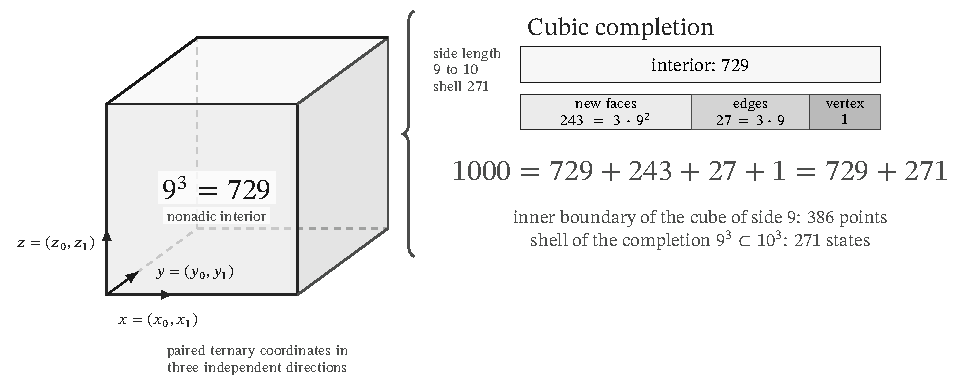
\includegraphics[width=\linewidth,keepaspectratio]{figures/cubo_emrh.pdf}
\caption{Cubic representation of the expansion from nine to ten classes per coordinate. Strata \(S_1,S_2,S_3\) locate the added incidences on faces, edges, and the apex; their cardinalities form the \(271\)-element shell. The \(386\)-element boundary belongs to the initial cube. This geometric perspective complements the partition in Figure~\ref{fig:revision-emrh}; graphical spacing is schematic.}
\label{fig:completacion-cubo-recuperado}
\end{figure}

% END IX03_CUBIC_COMPLETION_FIGURE

\subsubsection{Preservation of unity and dimensional compatibility}

Normalization is not limited to dividing an isolated identity. In dimension
\(d\), the product \(\widehat E^d\) carries the uniform measure
\(\mu_d(\{x\})=10^{-d}\). The coordinate projection
\(p_d:\widehat E^{d+1}\to\widehat E^d\) removes the last coordinate.

\begin{proposition}[Projective compatibility of the normalized measures]
For every \(d\geq1\),
\[
 (p_d)_*\mu_{d+1}=\mu_d,
 \qquad \mu_d(\widehat E^d)=1.
\]
The mass of the stratum with \(r\) additional coordinates is
\(\binom dr9^{d-r}/10^d\), and the sum of the masses of all strata
is one.
\end{proposition}
\begin{proof}
Each point of \(\widehat E^d\) has ten preimages. Their total mass is
\(10\,10^{-(d+1)}=10^{-d}\). Equality for any subset
follows by summing over its points. The stratified formula follows
from the same count as \eqref{eq:revision-estratos}; the binomial
\((9+1)^d\) gives the total normalization.
\end{proof}

In dimension three, removing the apex leaves mass \(999/1000\), and
restoring it adds \(1/1000\). Renormalizing before restoration
would define another measure: the distinction is operationally relevant.
In particular, preservation of probability mass, preservation of transport
registers, and thermodynamic dissipation are statements about
different objects. The proposition proves the first and provides the
compatible support for studying the second; the third requires a
specified dynamical and energetic realization.

The internal geometric boundary also remains distinct.
On the Cartesian representative \(\{1,\ldots,9\}^3\), removing
\(\{2,\ldots,8\}^3\) leaves \(386\) points. This boundary belongs to the
initial cube, whereas \(\widehat C\setminus C\) belongs to its
enlargement. The cubic completion, the positional base-thousand expansion, and
the exceptional incidence readout share support data;
their respective maps determine which information from those data
each representation uses.


% Fragmento conservado; véase MANIFIESTO_ANTECEDENTES_LECTURA.json.
% Incorporación al final de extension.tex; no contiene una sección principal.
% Procedencia: RESULTADO_RECUPERADO; explicitación sectorial de las hipótesis.
% Fuentes leídas: monografía Doble proyección holográfica (cantera editorial),
% manuscrito/local/01_tesis_recuperada.tex y
% manuscrito/generated/algebra_holonomica.tex, especialmente §§1--7 y 21.
% Definición rectora de número: manuscrito/flattened/main_autosuficiente.tex,
% secciones que comienzan en líneas 22137 y 23000 de la cantera de 775 páginas.
% No se adopta su presentación global como prueba de todas las flechas TPK.

\subsection{Number as a compatible section and value as a readout}
\label{hist:seccion}

The distinction between state and observation makes it possible to specify which object is
prolonged as resolution increases. At depth \(n\), let \(X_n\)
be the set of admissible states produced by APP--TRIT--TPK. Their data
include position, sum and product sheets, residues and quotients, regime,
orientation, carry, phase, route, boundary, memory, and survival. These are not
independent coordinates: preceding arithmetic evaluations and transports
impose their relations. A prolongation preserves those relations
in each antecedent, even as it adds new steps and new memory data.
This is the meaning of the arithmetic of histories developed in
\textup{(provenance preserved in the technical record)}.

Let \(r_{m,n}:X_m\to X_n\), for \(m\geq n\), be the depth
restrictions, with \(r_{n,n}=\operatorname{id}\) and
\(r_{\ell,n}=r_{m,n}\circ r_{\ell,m}\). Each restriction preserves the
prefix and the information already determined in it.

\begin{definition}[Compatible numerical section]
An HMT number is a compatible history of the state system:
\begin{equation}
 x=(x_n)_{n\geq0}\in X_\infty:=\varprojlim_n X_n,
 \qquad r_{m,n}(x_m)=x_n.
 \label{hist:limite-inverso}
\end{equation}
A readout is an additional operation on a specified domain of these
histories. A digit is a finite observation; a scalar value is an
evaluation of the readout. The pair consisting of the section and its readout constitutes
a read presentation, not a redefinition of the section's identity.
\end{definition}

On the Archimedean domain \(X_\infty^{\mathrm{Arch}}\), the readout associates
a closed cylinder with each prefix, preserves their nesting, and makes
their diameter tend to zero. It thus determines
\begin{equation}
 \operatorname{ev}_{\mathbb R}:X_\infty^{\mathrm{Arch}}\longrightarrow
 \mathbb R,\qquad
 \{\operatorname{ev}_{\mathbb R}(x)\}=\bigcap_n I_n(x).
 \label{hist:evaluacion}
\end{equation}
The concrete construction of these cylinders and the determination of their boundaries
are developed in Section~\ref{sec:generacion}. Definition
\eqref{hist:limite-inverso} does not by itself assert that the image of
\eqref{hist:evaluacion} is the entire line: a coverage assertion
requires its own theorem. Nor does equality of values establish, without
an injectivity result, equality of their histories. This separation
makes it possible to speak of precision as depth while preserving the difference
between the arithmetic antecedent and its scalar realization.

\subsection{Composition of histories and memory multiplier}
\label{hist:algebra}

Fix a sector of states at depth \(n\) and a category
\(\mathcal C\) whose arrows are their admissible histories. Composition
is written \(vu=v\circ u\): \(u\) is traversed first and then \(v\).
The elementary steps come from TPK selection, transport, and
updating. A local tritic fiber admits the expression
\(\mathbb R[J_x]/(J_x^2+\tau(x)1_x)\), where
\(\tau(x)\in\{+1,0,-1\}\). Regime and orientation belong to the
state being transported; a transition between regimes is not equivalent to
identifying their quadratic algebras.

The following formulation specifies an algebraic sector of this composition.
For each object \(x\), a unital associative real algebra \(A_x\) is given,
possibly noncommutative. For each \(u:x\to y\), a
unital homomorphism \(\rho_u:A_x\to A_y\) is given. We assume a strict action:
\begin{equation}
 \rho_{\operatorname{id}_x}=\operatorname{id}_{A_x},\qquad
 \rho_v\rho_u=\rho_{vu}.
 \label{hist:accion-estricta}
\end{equation}
For each composable pair \(u:x\to y\), \(v:y\to z\), fix an
invertible central multiplier
\(\Omega(v,u)\in Z(A_z)^\times\). We require the normalization
\(\Omega(\operatorname{id}_y,u)=\Omega(u,\operatorname{id}_x)=1_y\)
and, for each composable triple, the identity
\begin{equation}
 \rho_w\bigl(\Omega(v,u)\bigr)\Omega(w,vu)
   =\Omega(w,v)\Omega(wv,u).
 \label{hist:cociclo}
\end{equation}
These are explicit assumptions on the transports and their coefficients, not a
consequence of calling the dynamics holonomic. When this presentation is applied
to a TPK sector, its \(\rho_u\) and \(\Omega(v,u)\) must be identified.
Transitions expressed through bimodules require that structure to be
preserved and are not replaced by \eqref{hist:accion-estricta}.

The space of finite sums
\[
 \mathcal H(\mathcal C,A,\rho,\Omega)
   =\bigoplus_{u\in\operatorname{Mor}(\mathcal C)} A_{t(u)}T_u
\]
is equipped with the bilinear product
\begin{equation}
 (aT_v)(bT_u)=a\rho_v(b)\Omega(v,u)T_{vu},
 \label{hist:producto}
\end{equation}
if the arrows are composable, and zero otherwise. Here \(t(u)\)
denotes the terminal state. The sum brings together histories with coefficients; the
product concatenates histories while preserving the record multiplier.

\begin{proposition}[Sectorial associativity with a central multiplier]
Under \eqref{hist:accion-estricta} and \eqref{hist:cociclo}, the product
\eqref{hist:producto} is associative. If the set of objects is finite,
its unit is \(\sum_x1_xT_{\operatorname{id}_x}\).
\end{proposition}
\begin{proof}
For \(u:x\to y\), \(v:y\to z\), \(w:z\to t\), let
\(a\in A_y\), \(b\in A_z\), \(c\in A_t\). The two coefficients
of \(T_{wvu}\) are
\begin{align*}
 ((cT_w)(bT_v))(aT_u):\quad&
 c\rho_w(b)\Omega(w,v)\rho_{wv}(a)\Omega(wv,u),\\
 (cT_w)((bT_v)(aT_u)):\quad&
 c\rho_w(b)\rho_w\rho_v(a)\rho_w(\Omega(v,u))\Omega(w,vu).
\end{align*}
The strict action identifies \(\rho_w\rho_v(a)\) with \(\rho_{wv}(a)\).
Centrality of \(\Omega(w,v)\) allows it to be moved to the right of
that factor; \eqref{hist:cociclo} then equates the remaining products.
The coefficients \(a,b,c\) are not permuted. If the triple is not composable,
both parenthesizations are zero by their initial and terminal states.
Bilinearity completes the proof. The local identities and the
normalization of \(\Omega\) verify the indicated unit.
\end{proof}

The calendar carry provides an effective example. In the category
with one object and arrows \(C_9\), take coefficients
\(A=\mathbb R[z,z^{-1}]\), the identity action, and
\[
 \Omega(b,a)=z^{c_0(a,b)},\qquad
 c_0(a,b)=\left\lfloor\frac{a+b}{9}\right\rfloor,
 \quad 0\leq a,b<9.
\]
Both carry sums of a triple equal
\(\lfloor(a+b+c)/9\rfloor\); hence
\eqref{hist:cociclo} holds. The formal variable \(z\) records the winding without
assigning it a numerical value. Subsequently imposing \(z^{12}=1\) recovers the
dodecaphase record of the calendar \eqref{eq:extension108}; retaining
\(z\) without this relation distinguishes successive windings. The example realizes
the memory of this calendar, without identifying it with the entirety of
TPK memory.

\subsection{Double variance of refinement and conservation of unity}
\label{hist:doble-varianza}

Restricting states prolongs observables in the opposite direction.
Consider the function algebras, with pointwise product,
\(D_n=\operatorname{Fun}(X_n,\mathbb R)\). Precomposition defines
\begin{equation}
 r_{m,n}^*:D_n\longrightarrow D_m,
 \qquad r_{m,n}^*f=f\circ r_{m,n}.
 \label{hist:precomposicion}
\end{equation}
These are unital morphisms; they are also injective when the corresponding
restrictions are surjective. The direct limit
\(D_{\mathrm{cyl}}=\varinjlim_n(D_n,r_{n+1,n}^*)\) brings together
observations of finite depth. This algebra is not identified here
with the entire route algebra: prolonging the transport operators also requires
their compatibilities with refinement.

\begin{lemma}[Unity and naturality of evaluation]
If \(e_x\) is the indicator of \(x\in X_n\), then
\begin{equation}
 r_{m,n}^*e_x=\sum_{y:\,r_{m,n}(y)=x}e_y,
 \qquad r_{m,n}^*1_n=1_m,
 \label{hist:unidad}
\end{equation}
and, for every \(f\in D_n\), \(y\in X_m\),
\[
 \langle r_{m,n}^*f,y\rangle=\langle f,r_{m,n}y\rangle.
\]
Each section \(x\in X_\infty\) determines a well-defined evaluation
\(D_{\mathrm{cyl}}\to\mathbb R\), given by \([f]\mapsto f(x_n)\)
for \(f\in D_n\).
\end{lemma}
\begin{proof}
The fibers of \(r_{m,n}\) partition \(X_m\). Their
indicators are orthogonal and sum to \(1_m\), proving
\eqref{hist:unidad}. Naturality is the definition of precomposition.
Finally, \((r_{m,n}^*f)(x_m)=f(x_n)\), so that two compatible
representatives give the same evaluation in the direct limit.
\end{proof}

Global unity is the constant function one over all possibilities;
the individual section selects a compatible history. Preserving the
former does not mean immobilizing the latter. Refinement may increase
the number of extensions and the depth of each history while maintaining
unity and all evaluations of its antecedents.


\clearpage
% Preserved fragment; see MANIFIESTO_ANTECEDENTES_LECTURA.json.
\section{Coinductive generation of \texorpdfstring{\(\pi,\varphi,e\)}{pi, phi, e} to arbitrary depth}
\label{sec:generacion}

The six-block emission is a finite stage of the construction, not a complete decimal expansion. Its role is to produce regions with multiplicity, orientation, and transport rules. Prolongation must preserve these data and determine a compatible collection of prefixes of arbitrary length. The term \emph{generation} denotes this operation; \emph{genealogy} denotes the reconstruction of its dependencies. Both notions are involved, but they serve different purposes.

\subsection{Orbits, regions, and characters of closure, propagation, and self-scaling}

For a word \(w=(w_1,\ldots,w_6)\), define
\[
 r(w)=(w_3,w_1,w_2,w_5,w_6,w_4),\qquad
 s(w)=(w_4,w_5,w_6,w_1,w_2,w_3).
\]
We have \(r^3=s^2=I\) and \(srs=r^{-1}\); these permutations therefore realize the dihedral group \(D_3\). The action preserves the catalogue and the multiplicities and commutes with \(\Psi\). The quotient of the \(243\) visible words has \(43\) orbits: thirty-eight of cardinality six and five of cardinality three.

The closure class is recognized by a fibre predicate: its six orientations have five emissions per word, total multiplicity \(1008\), and distribution \(432+4\cdot144\). There is exactly one orbit with these properties in the catalogue. To specify the other two selections, write \(f(w)=\#\Psi^{-1}(w)\), \(m(w)=\sum_{U\in\Psi^{-1}(w)}\operatorname{mult}(U)\), and \(\nu(w)=(n_0,n_1,n_2)\). The additive diagonal class of an emission is \(d(U)=[i+j]_9\) in indices from zero to eight; its additive signature retains this class and the orientation \(ES\) or \(NO\). Let \(\mathcal D(\mathcal O)\) be the set of these classes for all emissions over an orbit.

Among the orbits of size six, the joint predicate
\[
 f(w)=1,\qquad m(w)=144\quad(w\in\mathcal O),\qquad
 \mathcal D(\mathcal O)=\{0,3,6\}
\]
leaves exactly six orbits. In this sector, the census \(\nu=(2,3,1)\), the same as for closure, uniquely selects propagation; the census \(\nu=(2,2,2)\) uniquely selects self-scaling. The diagonal support cannot be omitted: without it there are four balanced single-preimage orbits of multiplicity \(144\), not one. Finally, the existence of an emission with \(d=6\) and orientation \(ES\) selects one representative of each orbit and yields
\begin{equation}
 w^{\rm cl}=010211,\qquad w^{\rm pr}=201101,\qquad w^{\rm au}=121200.
 \label{eq:palabras-regionales}
\end{equation}
These symbols first designate regions of the catalogue. Scalar identification will be established through their readouts; they are not chosen because they coincide with digits of a known constant.

The closure word \(010211\) has the following five preimages:
\begin{center}\small
\begin{tabular}{@{}lll r@{}}\toprule
Six-block emission&Multiplicative signature&Role&Multiplicity\\\midrule
\(501,614,498,169,272,272\)&\(555555\)&transverse&432\\
\(810,923,870,169,272,272\)&\(339555\)&positive orientation&144\\
\(810,983,810,169,272,272\)&\(393555\)&positive orientation&144\\
\(870,923,810,169,272,272\)&\(933555\)&positive orientation&144\\
\(870,923,810,418,674,521\)&\(933717\)&oriented return&144\\\bottomrule
\end{tabular}
\end{center}
The multiplicity \(432\) and the constant signature \(555555\) characterize the transverse region. They do not identify the central position \((5,5)\) of APP. Confusing a six-window signature with a position in the support would erase the distinction between numerical region and electronic structure.

The microfibre also has a precise bipartite morphology. Each emission is a product of an additive cursor class and a multiplicative class. The three positive regions share the same additive class of eighteen conditions; together they contain three multiplicative classes of eight conditions each. The transverse region has a product \(18\times24\); the three positive regions taken together, another \(18\times24\); and the return, a product \(18\times8\). The decomposition by emissions has five parts, whereas the decomposition into connected components of the bipartite graph has three. Both preserve the same \(1008\) seeds without reducing form to a cardinality.

\subsection{Finite transport and the prolongation boundary}

The endomorphisms \(L_0,L_1\) of the ternary word space act before the Archimedean realization. Their determination begins with the transitions of the arithmetic state, not with the prescription of two matrices. If \(U_t\) is the composite step of selection, transport, and update, the observed block satisfies
\[
 b_j^\chi=\Pi_6(x_j^\chi),\qquad
 x_{j+1}^\chi=U_{9j+9}\cdots U_{9j+1}(x_j^\chi),
 \qquad \chi\in\{\mathrm{cl},\mathrm{pr},\mathrm{au}\}.
\]
Six transitions are formed for each regime: two consecutive transitions in each of the three regions. The pairs of source and target matrices obtained in the record are
\[
\begin{array}{c|c|c|c}
X_0&Y_0&X_1&Y_1\\\hline
010211&012222&010211&002111\\
012222&010211&002111&110221\\
201101&121221&102011&012222\\
121221&102011&012222&102011\\
121200&112202&121020&010210\\
112202&121020&010210&010200
\end{array}
\]
Each string of six digits represents a row in \(\FF_3^6\). Since \(\det X_0=1\) and \(\det X_1=-1\) in \(\FF_3\), the equations \(X_aL_a=Y_a\) uniquely determine \(L_a=X_a^{-1}Y_a\). In this row-vector chart, they yield
\[
 L_0=\begin{pmatrix}
 2&2&2&1&2&1\\2&1&2&2&1&1\\1&0&0&1&0&2\\
 0&0&1&1&1&0\\2&2&2&0&2&1\\2&1&2&1&0&0
 \end{pmatrix},\quad
 L_1=\begin{pmatrix}
 2&1&2&0&2&2\\1&2&1&1&2&0\\1&2&1&1&1&2\\
 0&1&0&0&2&1\\2&0&2&1&0&1\\0&2&2&2&1&1
 \end{pmatrix}\quad(\bmod3).
\]
The schedule \((L_0,L_0,L_1,L_1)\) produces four new blocks of six components. Their concatenations form
\[
 w_6\longrightarrow w_{12}\longrightarrow w_{18}
 \longrightarrow w_{24}\longrightarrow w_{30}.
\]
The subscripts of \(w\) indicate accumulated length. The boundary \(R_{36}\) preserves the terminal structure and opens the prolongation relation; it is not renamed as a final periodic block that could be repeated indefinitely.

The identity \(L=X^{-1}Y\) proves uniqueness once the transitions are fixed; it does not replace the production of those transitions by \(U_t\). The provenance of their record and the examination of the sixteen binary schedules are documented in the technical supplement. The indicated schedule is the only one of these sixteen that jointly reproduces the three sequences of five blocks.

\subsection{Five closure regions and angular compensation}

The closure region contains one transverse component and four accompanying components. The symmetric readout acts on the space of its five positions through
\[
 P_5=\frac15\mathbf1\mathbf1^{\mathsf T},\qquad
 \mathbf1=(1,1,1,1,1)^{\mathsf T}.
\]
Invariance \(P_5\lambda=\lambda\) and conservation \(\mathbf1^{\mathsf T}\lambda=1\) force \(\lambda=\mathbf1/5\). This normalization distributes the unit among positions of the readout; it does not replace the seed multiplicities \(432,144,144,144,144\) with uniform frequencies. The elliptic chart of the readout realizes each coordinate through \(1+\lambda_jJ\); its slope is \(\lambda_j\), so the primitive slope is \(1/5\). This makes explicit the rule taking a normalized coordinate to a slope, rather than identifying the two notions without a map. The readout composes the four accompanying positions by the law
\begin{equation}
 a\oplus b=\frac{a+b}{1-ab}.
 \label{eq:suma-pendientes}
\end{equation}
This law is obtained by multiplying \((1+aJ)(1+bJ)\) in the regime \(J^2=-I\) and dividing by its scalar component. The composition of slopes is therefore a realization of the quadratic structure of TRIT, not an ordinary sum of four fractions.

\begin{proposition}[Closure compensator]
The composition of four slopes \(1/5\) is \(120/119\). The condition of return to slope one determines a unique positive compensator of the form \(1/q\), with \(q>1\), and yields \(q=239\).
\end{proposition}
\begin{proof}
The first doubling gives \((1/5)\oplus(1/5)=5/12\); the second, \((5/12)\oplus(5/12)=120/119\). The condition
\[
 \frac{120/119-1/q}{1+(120/119)/q}=1
\]
is equivalent to \((120-119)q=120+119\), hence \(q=239\).
\end{proof}

The resulting closure character has the realization
\begin{equation}
 \Pi_{\rm cl}=4\left(4\arctan\frac15-\arctan\frac1{239}\right).
 \label{eq:lector-pi}
\end{equation}
Machin's angular identity recognizes \(\Pi_{\rm cl}=\pi\). The direction of the construction is precise: the slope and the number of compositions are specified by the pentafibre readout; the compensation equation forces \(239\). Once this character has been produced, its evaluation by alternating series does not select the seed orbit anew.

For \(0<x<1\), the alternating sums
\[
 A_n(x)=\sum_{j=0}^n\frac{(-1)^jx^{2j+1}}{2j+1}
\]
enclose \(\arctan x\) between two consecutive truncations, with difference \(x^{2n+3}/(2n+3)\). Applied to the two slopes in \eqref{eq:lector-pi}, they provide rational endpoints with explicit error bounds. The numerical value is thus calculated as a consequence of the exact character, without introducing a target prefix.

\subsection{Propagation readout and normalization of the unit}

The propagation region is realized by a formal collection \(P_t\in\mathcal A[[t]]\), where \(\mathcal A\) is a unital commutative algebra over \(\QQ\). Its composition satisfies \(P_{t+s}=P_tP_s\), with unit \(P_0=1\), and the oriented elementary transport fixes the scalar generator \(P'_0=+1\). The condition fixes its sign, not merely its magnitude. Writing
\[
 P_t=\sum_{n\ge0}a_nt^n,
\]
the normalization determines \(a_0=a_1=1\). Comparing the coefficient of \(s^nt\) in \(P_{s+t}=P_sP_t\) gives \((n+1)a_{n+1}=a_na_1\); equivalently, \(P'_t=P_t\). Thus,
\begin{equation}
 (n+1)a_{n+1}=a_n,\qquad a_n=\frac1{n!}.
 \label{eq:propagacion}
\end{equation}
The character at one unit of the parameter is \(\Pi_{\rm pr}=P_1\), subsequently recognized as \(e\).

Normalization of the generator matters. Without this datum, the semigroup law would admit \(P_t=e^{ct}\) for different \(c\); the condition fixing the unit of the parameter in the readout is therefore not omitted. This condition precedes decimal comparison and belongs to the exposition of the operational rule, not to the choice of an experimental value.

\begin{proposition}[Rational propagation bounds]
For \(n\ge1\), let \(E_n=\sum_{j=0}^n1/j!\). Then
\[
 E_n<\Pi_{\rm pr}<E_n+\frac{n+2}{(n+1)(n+1)!}.
\]
\end{proposition}
\begin{proof}
The first omitted term is \(1/(n+1)!\). Each subsequent ratio is at most \(1/(n+2)\). The geometric upper bound for the tail is
\[
 \frac1{(n+1)!}\frac1{1-1/(n+2)}
 =\frac{n+2}{(n+1)(n+1)!}.
\]
Strict inequality follows from the decrease of the successive ratios.
\end{proof}

\subsection{Modal incidence and generation of self-scaling}

The tritic selector produces the cycle \((+1,-1,0)\). On the modes \(\Sigma,\Pi\), the rule is \(+1:m\mapsto\Sigma\), \(-1:m\mapsto\Pi\), \(0:m\mapsto m\). With cyclic closure, the observed mode is \((\Sigma,\Pi,\Pi)\). Its edges are \(\Sigma\to\Pi\), \(\Pi\to\Pi\), and \(\Pi\to\Sigma\). Its incidence, in this ordering of the modes, is therefore
\begin{equation}
 F_{\rm av}=\begin{pmatrix}0&1\\1&1\end{pmatrix}.
 \label{eq:fav}
\end{equation}
The four entries are obtained from the schedule, not from an equation that has already received the value of \(\varphi\). Repeating the schedule gives counts \(3F_{\rm av},9F_{\rm av},36F_{\rm av}\) at lengths nine, twenty-seven, and one hundred and eight. These counts are not powers of the matrix.

\begin{theorem}[Positive self-scaling character]
The incidence \eqref{eq:fav} has a unique strictly positive eigenray. When normalized as \((1,x)^{\mathsf T}\), its coordinate \(x\) satisfies \(x^2-x-1=0\), \(x>0\), and equals \(\varphi=(1+\sqrt5)/2\).
\end{theorem}
\begin{proof}
The eigenvalue equation gives \(x=\lambda\) and \(1+x=\lambda x\). Eliminating \(\lambda\) yields the polynomial. Only one of its two roots is positive. Since all entries of \(F_{\rm av}^2\) are positive, the positive ray is unique and simple. The radical expression recognizes the coordinate obtained; it does not participate in the production of \(F_{\rm av}\).
\end{proof}

With \(F_0=0,F_1=1,F_{n+1}=F_n+F_{n-1}\), the incidence induces, for \(n\geq1\),
\[
 F_{\rm av}^n=\begin{pmatrix}F_{n-1}&F_n\\F_n&F_{n+1}\end{pmatrix}.
\]
The consecutive ratios \(F_{n+1}/F_n\) alternate around \(\varphi\). The determinant identity
\[
 F_{n+1}^2-F_nF_{n+2}=(-1)^n
\]
gives an exact width \(1/(F_nF_{n+1})\) between two consecutive ratios. Their growth makes this rational bracket arbitrarily narrow.

\subsection{Compatible cylinders and arbitrary depth}

The realization of a ternary block \(b=(b_1,\ldots,b_6)\) is the integer
\[
 \nu(b)=\sum_{j=1}^6b_j3^{6-j}\in\{0,\ldots,728\}.
\]
A sequence of blocks defines integer prefixes by \(N_{n+1}=729N_n+\nu(b_{n+1})\), starting from \(N_0=m\), where \(m\) is the integer part determined by the readout. The preceding brackets place the closure, propagation, and self-scaling characters in \((3,4)\), \((2,3)\), and \((1,2)\), respectively; their initial values are therefore \(m=3,2,1\). Subsequent blocks refine the fractional part. The corresponding cylinder is
\begin{equation}
 I_n=\left[\frac{N_n}{729^n},\frac{N_n+1}{729^n}\right],
 \qquad |I_n|=729^{-n}.
 \label{eq:cilindro}
\end{equation}
The half-open convention is used to select a representative when a value lies on a boundary. Passage to the limit uses the closures of these intervals and identifies the two equivalent boundary expansions. This qualification prevents the assumption that every intersection of nested half-open intervals is automatically nonempty.

\begin{theorem}[Determination of the scalar realization]
A compatible block history determines a unique limit of the left endpoints of \eqref{eq:cilindro}. If an exact character has rational brackets of arbitrarily small width and is separated from the boundary of every decimal cylinder examined, each decimal prefix of finite length is determined after a finite computation. The prefixes thus obtained are mutually compatible.
\end{theorem}
\begin{proof}
Extending a block preserves the previous prefix by Euclidean division. The closed cylinders are nested and their diameter tends to zero; their left endpoints form a Cauchy sequence and have a unique limit. For a fixed decimal length, a value separated from the boundaries of the partition has positive distance from them. A sufficiently narrow bracket lies within a single cell and determines its prefix. Uniqueness of the cell and nesting of the partitions prove compatibility under truncation. At points with a terminating expansion, the exact boundary decision and its representation convention must be added; this decision does not follow from numerical width alone.
\end{proof}

\begin{corollary}[Finite determination and compatibility of regional prefixes]
\label{gen:prefijos-regionales}
For each of the realizations \(\pi,\varphi,e\) and every finite
decimal length, the constructed brackets determine the corresponding prefix
by a finite computation. The prefixes obtained at different depths
are compatible under truncation.
\end{corollary}
\begin{proof}
The closure, propagation, and self-scaling characters have the
preceding brackets. After their recognition, the irrationality of \(\pi,e,\varphi\)
ensures their separation from the rational boundaries of every finite decimal
partition. The preceding theorem applies to each character.
\end{proof}
Arbitrary depth expresses the quantifier in the corollary: for every
finite horizon there is a computation determining its prefix. The mathematical
object is the complete compatible collection; each execution obtains a
finite projection of it.

\subsection{Specular involution and synchronization of the regions}

The joint nonadic connection transports the three characters together. In the ninth-phase chart, the self-scaling axis and the ternary sum of closure and propagation remain fixed under specular interchange. Helical inversion changes the direction of transport; the mirror of the two channels changes their relative orientation. These are different involutions, although both act on the same trajectory system.

The matching census values illustrate this coordination:
\begin{center}
\begin{tabular}{@{}c rrr l@{}}\toprule
Phase&\(N_\pi\)&\(N_e\)&\(N_\varphi\)&Equality of counts\\\midrule
4&207&207&122&\(N_\pi=N_e\)\\
5&39&151&151&\(N_e=N_\varphi\)\\
6&110&110&69&\(N_\pi=N_e\)\\
7&81&29&81&\(N_\varphi=N_\pi\)\\
8&59&59&59&triple synchronization\\
9&43&43&43&triple synchronization\\\bottomrule
\end{tabular}
\end{center}
These integers count compatible coordinates of the regions. They do not assert equality between \(\pi\), \(e\), and \(\varphi\) as real numbers. If
\[
 \partial(a,b,c)=(a-b,b-c,c-a),
\]
its image belongs to the lattice \(A_2=\{(u,v,w)\in\ZZ^3:u+v+w=0\}\). In phases eight and nine the relative component vanishes, but the diagonal component changes from \((59,59,59)\) to \((43,43,43)\). Relative synchronization coexists with a shift of \(-16\) per channel. The closure that will lead to \(\alpha\) must preserve both pieces of information: relative coincidence and memory evolution.


% Fragmento conservado; véase MANIFIESTO_ANTECEDENTES_LECTURA.json.
\subsection{Mirror symmetry of the regions and double realization}
\label{mono-ampl:regiones}

The mirror exchange acts on the regional block
\(B=(u^\pi,u^e,u^\varphi)\in(\mathbb F_3^6)^3\) by
\[
 \mathfrak cB=(u^e,u^\pi,u^\varphi).
\]
Its fixed axis and aggregate are, respectively, \(u^\varphi\) and
\(s=u^\pi+u^e\). This fixedness concerns the involution on a fiber;
both coordinates may evolve during nonadic transport.
With \(q=u^\pi+u^e+u^\varphi\),
\(a=u^\pi+u^e-u^\varphi\), and \(d=u^\pi-u^e\), one recovers
\[
 u^\varphi=2(q-a),\qquad s=q-u^\varphi,\qquad
 u^\pi=2(s+d),\qquad u^e=2(s-d).
\]
The equalities hold componentwise in \(\mathbb F_3\), where
\(2^{-1}=2\). The mirror preserves \(q,a,s\) and reverses \(d\); this
antisymmetric coordinate individualizes the distribution preserved
by the aggregate without distinction. The inversion \(\mathcal I\) of the time index and the
channel involution \(\mathfrak c\) consequently act on
different data.

Phase return has an explicit witness:
\[
 \begin{aligned}
 B_1&=(012222\mid121221\mid112202),\\
 B_{10}&=(101222\mid112221\mid112002).
 \end{aligned}
\]
Both positions have phase \(1\); the block, axis, and memory have
changed. Likewise, synchronization of the censuses at phases \(8\) and
\(9\) cancels their relative differences, while the diagonal component
changes from \((59,59,59)\) to \((43,43,43)\). Equality of a relative observable
does not exhaust the state determining it.

The double realization preserves this architecture. In Section
8.1 of Article I (provenance of the exceptional corridor, preserved in the technical record), the same prefix determines nested
cylinders on the one hand and a sequence of encoded words with their frames on the other.
The first map passes to the limit through contraction of diameters; the second
satisfies \(r_{n,m}Q_n=Q_mp_{n,m}\) and defines \(Q_\infty\).
Figure \ref{mono-ampl:fig-regional} anticipates these two maps.
The subsequent incidence progression constructs codes, lattices, and the
Moonshine realization on their own domains; the automorphism group
acts on that realization, not on the digits through an
implicit identification.

% Fragmento conservado; véase MANIFIESTO_ANTECEDENTES_LECTURA.json.
% Figura acumulativa; destino figures/monodromia_regional_ampliacion.tex.
\begin{figure}[!htbp]
\centering
\begin{tikzpicture}[x=1cm,y=1cm,>=Latex,font=\small,
  flow/.style={->,line width=.55pt},
  ann/.style={align=center,font=\footnotesize}]
\node[font=\bfseries] at (6.9,9.2)
  {Nonadic connection and regional coordinates};
\begin{scope}[shift={(3.4,6.8)}]
 \foreach \k in {1,...,9}{
  \pgfmathsetmacro{\ang}{90-40*(\k-1)}
  \coordinate (p\k) at (\ang:1.52);
  \fill (p\k) circle (1.4pt);
  \node[fill=white,inner sep=1.1pt,font=\footnotesize]
    at (\ang:1.83) {\(\k\)};
 }
 \foreach \k in {1,...,8}{
  \pgfmathtruncatemacro{\next}{\k+1}
  \draw[flow,shorten >=3pt,shorten <=3pt] (p\k)--(p\next);
 }
 \draw[flow,shorten >=3pt,shorten <=3pt] (p9)--(p1);
 \node[ann] at (0,.1) {\(g_k\in C_9\)\\\(\Gamma_{9,k}\)};
 \node[ann] at (0,-2.23) {One winding: \(g\mapsto g\), \(m\mapsto m+1\)};
\end{scope}
\node[ann,text width=5.25cm] at (10.1,7.75)
 {\(B_k=(u_k^\pi,u_k^e,u_k^\varphi)\)\\
 regional block in a fibre};
\node at (8.55,6.5) {\(u^\pi\)};
\node at (11.65,6.5) {\(u^e\)};
\draw[<->,line width=.65pt] (8.95,6.5)--node[above]{\(\mathfrak c\)}(11.25,6.5);
\draw[densely dashed,gray] (10.1,5.72)--(10.1,7.23);
\node[fill=white,inner sep=2pt] at (10.1,5.6){\(u^\varphi\)};
\node[ann] at (10.1,4.6)
 {Axis \(u^\varphi\) and aggregate \(u^\pi+u^e\)\\
 invariant under \(\mathfrak c\)};
\draw[flow] (5.45,6.8)--(7.25,6.8);
\draw[gray!60,line width=.3pt] (.55,4.02)--(13.25,4.02);
\node[ann,text width=12cm] (hist) at (6.9,3.47)
 {Compatible history: prefixes, cylinders, orientation, quotients,
 incidence frames and memory};
\coordinate (fork) at (6.9,2.85);
\draw[flow] (hist.south)--(fork);
\draw[flow] (fork)--(3.6,2.2);
\draw[flow] (fork)--(10.3,2.2);
\node[ann,text width=5.6cm] at (3.6,1.65)
 {Archimedean realization\\
 \(I_{n+1}\subseteq I_n,\quad |I_n|=729^{-n}\)\\
 limit of the regional prefixes};
\node[ann,text width=5.6cm] at (10.3,1.65)
 {Incidence realization\\
 \(r_{n,m}Q_n=Q_mp_{n,m}\)\\
 encoded words and compatible frames};
\node[ann,text width=5.6cm] at (3.6,.42)
 {\(\pi,\varphi,e\); dodecaphasic determination of \(\alpha\)};
\node[ann,text width=5.6cm] at (10.3,.42)
 {Witt--Golay--Leech--\(V^\natural\)\\
 automorphisms of the exceptional realization};
\draw[flow] (3.6,1.03)--(3.6,.78);
\draw[flow] (10.3,1.03)--(10.3,.78);
\end{tikzpicture}
\caption{\fontsize{9}{11}\selectfont Nine phases of a connection and two realizations of the compatible
history. The cycle represents phase; each winding increments the counter.
The regional diagram represents the involution \(\mathfrak c\), which
interchanges closure and propagation and fixes the self-scale axis in a fibre.
This invariance does not require the axis to remain constant during transport.
The two lower maps use the same prefix: one determines
its numerical limit and the other preserves words and incidence frames. The
maps of this second realization are specified in Section
8.1 of Article I (provenance of the exceptional corridor, preserved in the technical register); the exceptional route is developed afterwards.}
\label{mono-ampl:fig-regional}
\end{figure}


\clearpage
% BEGIN NUCLEO_ADITIVO_20260921_SELECCION
\clearpage
% Demonstrative expansion DF003--DF007. The integral source is unchanged.
% Common owner of the Lean files cited in these comments:
% output/PAQUETE_ARTICULO_I_INTEGRACION_ESTADO_CAMPOS_20260919/.
% Causal placement of the first section: after the coinductive regional
% readers and before their registers are used as inputs to K selection.
% Causal placement of the second section: after the marked
% Paley--Witt--Golay--Leech construction and before reconstruction of the VOA.
% Both expository cuts preserve the same APP--TRIT--TPK origin.

\section[Regional generation and refinement]{Integral compatibility of regional generation, cylindrical refinement, and incidence}
\label{act21:sec:df-lectores-cilindros}

Regional prolongation produces ordered sequences of blocks together with
their reading depths. The Archimedean projection and ternary incidence
are calculated on these same sequences. The connection between the two
realizations can be formulated entirely through integer operations:
selection by rational intervals, Euclidean division, lifting of six
trits, carry reading, and the Witt transformation. This formulation makes
it possible to trace each coefficient from its generating block to its
subsequent use.

The construction uses the three regional readers already obtained from the
APP--TRIT--TPK state. We denote them by the indices
\(c\in\{\mathrm P,\mathrm E,\mathrm F\}\), corresponding, respectively,
to the closure, propagation, and autoscaling regions. Their real realization
will be written as \(v_c\). The subsequent identifications
\(v_{\mathrm P}=\pi_{\mathrm{HMT}}\),
\(v_{\mathrm E}=e_{\mathrm{HMT}}\), and
\(v_{\mathrm F}=\varphi_{\mathrm{HMT}}\) preserve this causal order.
The operation that emits a block inspects the rational intervals of the
regional reader; the real value enters the proof of correctness of that
operation.

\subsection{Positional emission through rational separation of cells}
\label{act21:subsec:df-emision-racional}

% Source: lean/biblioteca/RegionalPublicationComposition.lean,
% produced_brackets, eventual_publication, joint_eventual_publication,
% search_terminates, stopped_cell_correct, publications_compatible.

For each region, two rational sequences
\(\ell_c(j),u_c(j)\), constructed by its reader, are available and satisfy
\[
 \ell_c(j)\leq v_c\leq u_c(j).
\]
The cell-separation property proved for these readers states that, for
each integer \(s>0\), there exists \(J\) such that, for every \(j\geq J\),
\begin{equation}
 \lfloor s\ell_c(j)\rfloor
 =\lceil su_c(j)\rceil-1
 =\lfloor sv_c\rfloor.
 \label{act21:eq:df-separacion-celdas}
\end{equation}
Avoidance of rational boundaries by the regional values is the hypothesis
of the preceding theorems that guarantees this separation. Here we use
their operational conclusion together with the readers and intervals
that produce it.

\begin{definition}[Separation index and emitted prefix]
For \(s>0\), let
\[
 j_c(s)=\min\{j\in\mathbb N:
 \lfloor s\ell_c(j)\rfloor=\lceil su_c(j)\rceil-1\}.
\]
For an integer base \(b\geq2\) and a depth \(n\geq0\), define
\begin{equation}
 P_c(b,n)=\lfloor b^n\ell_c(j_c(b^n))\rfloor.
 \label{act21:eq:df-publicacion-prefijo}
\end{equation}
The prefix contains the integer part and the first \(n\) positions in base
\(b\); consequently, \(P_c(b,0)\) is the regional integer part.
\end{definition}

\begin{theorem}[Termination and correctness of emission]
\label{act21:thm:df-emision-correcta}
The index \(j_c(s)\) exists for every \(s>0\). The emitted prefixes satisfy
\begin{equation}
 P_c(b,n)=\lfloor b^n v_c\rfloor,
 \qquad
 P_c(b,n)\leq b^n v_c<P_c(b,n)+1.
 \label{act21:eq:df-prefijo-correcto}
\end{equation}
For each scale \(s\), a single sufficiency index \(J(s)\) can also be
chosen that is valid simultaneously for all three regions.
\end{theorem}

\begin{proof}
The eventual equality in \eqref{act21:eq:df-separacion-celdas} makes the set
defining \(j_c(s)\) nonempty. Its minimum exists by the well-ordering of
\(\mathbb N\). At any index where the equality holds, the rational lower
bound gives
\(\lfloor s\ell_c(j)\rfloor\leq\lfloor sv_c\rfloor\).
The upper bound, together with avoidance of a cell boundary, gives
\(\lfloor sv_c\rfloor\leq\lceil su_c(j)\rceil-1\).
When the two integer endpoints coincide, the intervening integer coincides
with them. This proves \eqref{act21:eq:df-prefijo-correcto}. For the joint
statement, it suffices to take the maximum of the three sufficiency indices
obtained at the same scale. The joint index controls all three emissions
simultaneously, while each region retains its own intervals.
\end{proof}

\begin{proposition}[Exact compatibility of prefixes]
\label{act21:prop:df-prefijos-compatibles}
For \(n,m\geq0\),
\begin{equation}
 \left\lfloor\frac{P_c(b,n+m)}{b^m}\right\rfloor=P_c(b,n).
 \label{act21:eq:df-truncamiento}
\end{equation}
In particular, the next block
\(d_c(b,n)=P_c(b,n+1)\bmod b\) satisfies
\begin{equation}
 P_c(b,n+1)=bP_c(b,n)+d_c(b,n),\qquad 0\leq d_c(b,n)<b.
 \label{act21:eq:df-paso-posicional}
\end{equation}
\end{proposition}

\begin{proof}
Write \(b^n v_c=N+\theta\), with
\(N=P_c(b,n)\) and \(0\leq\theta<1\). Then
\(P_c(b,n+m)=b^mN+\lfloor b^m\theta\rfloor\), and the second summand
belongs to \(\{0,\ldots,b^m-1\}\). Euclidean division by \(b^m\)
recovers \(N\). The specialization \(m=1\) yields
\eqref{act21:eq:df-paso-posicional} and its residual bound.
\end{proof}

\subsection{Regional blocks of six trits at arbitrary depth}
\label{act21:subsec:df-bloques-arbitrarios}

% Source: deltas/integracion/JointRegionalFrontier.lean,
% publish_base729_eq_base3, generated_block_from_longer_prefix,
% generated_block_eq_finite, generated_signature_eq_finite.

The integer equality \(729=3^6\) determines the grouping of six ternary
positions into a block. For \(t\geq0\), define
\begin{equation}
 u_c(t)=P_c(729,t+1)\bmod729,
 \qquad
 B_{c,j}(t)=
 \left\lfloor\frac{u_c(t)}{3^{5-j}}\right\rfloor\bmod3,
 \quad 0\leq j<6.
 \label{act21:eq:df-bloque-y-banda}
\end{equation}
Thus \(B_c(t)\) is an ordered word of six trits, and
\begin{equation}
 u_c(t)=\sum_{j=0}^{5}B_{c,j}(t)3^{5-j}.
 \label{act21:eq:df-elevacion-banda}
\end{equation}
The word and its integer lift are mutually recoverable representations
of the same emitted block.

\begin{theorem}[Stability of extraction at any depth]
\label{act21:thm:df-bloque-estable}
For every \(n\),
\[
 P_c(729,n)=P_c(3,6n).
\]
If \(t<n\), then
\begin{equation}
 u_c(t)=
 \left\lfloor\frac{P_c(729,n)}{729^{n-t-1}}\right\rfloor\bmod729.
 \label{act21:eq:df-bloque-prefijo-largo}
\end{equation}
Consequently, every extension of the prefix preserves all previously
emitted blocks and all signatures calculated from them.
\end{theorem}

\begin{proof}
The first equality follows because both prefixes are separated at the same
scale, \(729^n=3^{6n}\), and from
Theorem~\ref{act21:thm:df-emision-correcta}. For the second, apply
\eqref{act21:eq:df-truncamiento} at depths \(n\) and \(t+1\), and then take
the residue modulo \(729\). The ternary extraction in
\eqref{act21:eq:df-bloque-y-banda} is deterministic. Any explicit function of
those eighteen coordinates therefore retains the same result when the
prefix is extended.
\end{proof}

The construction is quantified over \(t\in\mathbb N\). A table
materializing one hundred blocks is a finite evaluation of this
construction; formula \eqref{act21:eq:df-bloque-prefijo-largo} determines its
compatibility with every subsequent extension exactly.

\begin{example}[First joint block]
Evaluation of the selected regional readers gives the words
\[
 B_{\mathrm P}(0)=010211,\qquad
 B_{\mathrm E}(0)=201101,\qquad
 B_{\mathrm F}(0)=121200.
\]
Their lifting by \eqref{act21:eq:df-elevacion-banda} produces
\[
 u_{\mathrm P}(0)=103,\qquad
 u_{\mathrm E}(0)=523,\qquad
 u_{\mathrm F}(0)=450.
\]
For example,
\(201101_3=2\cdot243+27+9+1=523\).
All six positions, including leading zeros, are retained in the band
representation. The leading zero in \(010211\) has a defined position
even though the decimal notation for \(103\) does not contain it.
\end{example}

\subsection{Transition registers and reconstruction of linear lifts}
\label{act21:subsec:df-registros-transicion}

% Sources: deltas/integracion/RegionalTransitionRecords.lean and
% GeneratedTransitionRecords.lean; lean/biblioteca/TPKLifts.lean.
% The reconstructed links are R(0)->R(1) and R(2)->R(3).

Over \(\mathbb F_3\), collect two consecutive emissions from each region
in the matrix
\begin{equation}
 R(t)=
 \begin{pmatrix}
 B_{\mathrm P}(t)\\ B_{\mathrm P}(t+1)\\
 B_{\mathrm E}(t)\\ B_{\mathrm E}(t+1)\\
 B_{\mathrm F}(t)\\ B_{\mathrm F}(t+1)
 \end{pmatrix}.
 \label{act21:eq:df-registro-matricial}
\end{equation}
This definition fixes both the regional order and the temporal order.
The first four registers are
\[
 X_0=R(0),\quad Y_0=R(1),\quad X_1=R(2),\quad Y_1=R(3).
\]
Their values, obtained by extraction from the regional prefixes, are
\begin{align*}
 X_0&=\begin{pmatrix}
0&1&0&2&1&1\\0&1&2&2&2&2\\2&0&1&1&0&1\\
1&2&1&2&2&1\\1&2&1&2&0&0\\1&1&2&2&0&2
\end{pmatrix},&
 Y_0&=\begin{pmatrix}
0&1&2&2&2&2\\0&1&0&2&1&1\\1&2&1&2&2&1\\
1&0&2&0&1&1\\1&1&2&2&0&2\\1&2&1&0&2&0
\end{pmatrix},\\[1ex]
 X_1&=\begin{pmatrix}
0&1&0&2&1&1\\0&0&2&1&1&1\\1&0&2&0&1&1\\
0&1&2&2&2&2\\1&2&1&0&2&0\\0&1&0&2&1&0
\end{pmatrix},&
 Y_1&=\begin{pmatrix}
0&0&2&1&1&1\\1&1&0&2&2&1\\0&1&2&2&2&2\\
1&0&2&0&1&1\\0&1&0&2&1&0\\0&1&0&2&0&0
\end{pmatrix}.
\end{align*}

\begin{theorem}[Unique reconstruction of the two initial links]
\label{act21:thm:df-elevaciones-reconstruidas}
The equations \(X_0L_0=Y_0\) and \(X_1L_1=Y_1\) each have a unique
solution in \(M_6(\mathbb F_3)\). These solutions are
\begin{align*}
 L_0&=\begin{pmatrix}
2&2&2&1&2&1\\2&1&2&2&1&1\\1&0&0&1&0&2\\
0&0&1&1&1&0\\2&2&2&0&2&1\\2&1&2&1&0&0
\end{pmatrix},&
 L_1&=\begin{pmatrix}
2&1&2&0&2&2\\1&2&1&1&2&0\\1&2&1&1&1&2\\
0&1&0&0&2&1\\2&0&2&1&0&1\\0&2&2&2&1&1
\end{pmatrix}.
\end{align*}
Both matrices are invertible.
\end{theorem}

\begin{proof}
The matrices
\begin{align*}
 A_0&=\begin{pmatrix}
1&1&2&0&1&2\\0&0&1&0&0&1\\2&1&2&1&0&1\\
0&2&0&1&0&2\\2&1&1&0&2&2\\2&1&1&1&1&2
\end{pmatrix},&
 A_1&=\begin{pmatrix}
1&0&1&2&0&0\\0&0&1&1&2&2\\0&1&2&0&1&1\\
1&1&0&2&0&0\\1&1&2&1&1&2\\1&0&0&0&0&2
\end{pmatrix}
\end{align*}
satisfy \(A_iX_i=X_iA_i=I\), by multiplication in \(\mathbb F_3\).
The solutions are therefore forced by \(L_i=A_iY_i\); multiplication
produces the two displayed matrices. Their inverses are
\begin{align*}
 L_0^{-1}&=\begin{pmatrix}
1&2&0&2&0&2\\2&0&2&2&0&0\\2&1&2&0&2&0\\
1&0&0&0&2&0\\0&2&1&1&2&0\\2&2&2&2&2&2
\end{pmatrix},&
 L_1^{-1}&=\begin{pmatrix}
2&0&2&1&2&1\\2&1&0&0&2&0\\2&0&2&2&0&2\\
2&0&0&1&1&0\\1&1&1&1&1&0\\2&0&1&2&2&0
\end{pmatrix}.
\end{align*}
The bilateral verification \(L_iL_i^{-1}=L_i^{-1}L_i=I\) proves exact
recovery of each transformed word. All products use residues \(0,1,2\)
with their interpretation in \(\mathbb F_3\).
\end{proof}

The causal reading of this result is precise: the regional emissions
produce \(R(t)\); the registers \(R(0),\ldots,R(3)\) determine the two
lifts above; their inverses recover the transformed words. Continuity
for every \(t\) belongs to the coinductive readers and
Theorem~\ref{act21:thm:df-bloque-estable}. The matrix reconstruction proved here
has the two links specified in its statement as its domain.

\subsection{Simultaneous refinement in ternary and decimal bases}
\label{act21:subsec:df-cilindros-mixtos}

% Source: deltas/integracion/RegionalCylinderTransition.lean.

A ternary emission of six trits and a decimal emission of three digits
are readings in different bases. To preserve their relationship, record
the state
\[
 s=(n,k,N,D),
\]
where \(N\) is a prefix at depth \(n\) in base \(729\), and \(D\) is
a prefix at depth \(k\) in base \(1000\). Their Archimedean cylinders are
\begin{equation}
 I_{729}(s)=\left[\frac{N}{729^n},\frac{N+1}{729^n}\right),\qquad
 I_{1000}(s)=\left[\frac{D}{1000^k},\frac{D+1}{1000^k}\right).
 \label{act21:eq:df-cilindros}
\end{equation}
The half-open upper endpoint assigns each value to a unique cell at a
given base and depth.

\begin{definition}[Integer compatibility defects]
Define
\begin{align}
 A(s)&=N1000^k-D729^n,\label{act21:eq:df-defecto-inferior}\\
 B(s)&=(N+1)1000^k-D729^n=A(s)+1000^k.
 \label{act21:eq:df-defecto-superior}
\end{align}
The state is compatible when
\begin{equation}
 A(s)<729^n,\qquad B(s)>0.
 \label{act21:eq:df-compatibilidad}
\end{equation}
\end{definition}

\begin{lemma}[Integer criterion for intersection]
The cylinders in \eqref{act21:eq:df-cilindros} have a nonempty intersection if
and only if \eqref{act21:eq:df-compatibilidad} holds.
\end{lemma}

\begin{proof}
Two half-open intervals \([a,b)\) and \([c,d)\), with \(a<b\) and
\(c<d\), intersect exactly when \(a<d\) and \(c<b\). Applying this
condition to \eqref{act21:eq:df-cilindros} and multiplying by the positive
denominators gives
\(N1000^k<(D+1)729^n\) and
\(D729^n<(N+1)1000^k\). These are the two inequalities in
\eqref{act21:eq:df-compatibilidad}.
\end{proof}

\begin{definition}[Update of depths and prefixes]
For \(0\leq u<729\) and \(0\leq d<1000\), define
\begin{align*}
 T_u(n,k,N,D)&=(n+1,k,729N+u,D),\\
 T_{u,d}(n,k,N,D)&=(n+1,k+1,729N+u,1000D+d).
\end{align*}
The first operation refines only the ternary cylinder. The second refines
both readings and preserves both depths in the state.
\end{definition}

\begin{proposition}[Exact boundary recurrences]
\label{act21:prop:df-rec-frontera}
The updates above satisfy
\begin{align}
 A(T_u s)&=729A(s)+u1000^k,\label{act21:eq:df-rec-ternaria}\\
 A(T_{u,d}s)&=729000A(s)+u1000^{k+1}-d729^{n+1}.
 \label{act21:eq:df-rec-conjunta}
\end{align}
\end{proposition}

\begin{proof}
For the first identity,
\[
 (729N+u)1000^k-D729^{n+1}
 =729(N1000^k-D729^n)+u1000^k.
\]
For the second,
\begin{align*}
 &(729N+u)1000^{k+1}-(1000D+d)729^{n+1}\\
 &\qquad=729000(N1000^k-D729^n)
      +u1000^{k+1}-d729^{n+1}.
\end{align*}
Both are integer identities preceding any real approximation.
\end{proof}

\begin{theorem}[Refinement of the generated regional cylinders]
\label{act21:thm:df-refinamiento-generado}
Let
\[
 s_c(n,k)=(n,k,P_c(729,n),P_c(1000,k)).
\]
Then \(s_c(n,k)\) is compatible for all \(n,k\). Moreover,
\begin{align*}
 T_{u_c(n)}s_c(n,k)&=s_c(n+1,k),\\
 T_{u_c(n),d_c(1000,k)}s_c(n,k)&=s_c(n+1,k+1).
\end{align*}
Euclidean division of the refined prefixes recovers the preceding
prefixes exactly. For every \(a,b\geq0\),
\[
 \frac{P_c(729,n+a)-P_c(729,n+a)\bmod729^a}{729^a}
 =P_c(729,n),
\]
and the analogous identity holds in base \(1000\).
\end{theorem}

\begin{proof}
Theorem~\ref{act21:thm:df-emision-correcta} places \(v_c\) simultaneously in
both intervals in \eqref{act21:eq:df-cilindros}; the intersection criterion
gives compatibility. The update identities are
\eqref{act21:eq:df-paso-posicional} in each base. Recovery follows from
\eqref{act21:eq:df-truncamiento}. Thus the defect recurrence and prefix
recovery are consequences of the same update.
\end{proof}

\begin{example}[First pair of regional cylinders]
For \(n=k=1\), evaluation of the three regions gives
\[
\begin{array}{c|rr|rr}
 c&N&D&A&B\\\hline
 \mathrm P&2290&3141&211&1211\\
 \mathrm E&1981&2718&-422&578\\
 \mathrm F&1179&1618&-522&478
\end{array}
\]
In all three rows, \(A<729\) and \(B>0\). The first prefix column
decomposes as \(2290=3\cdot729+103\),
\(1981=2\cdot729+523\), and \(1179=729+450\): exactly the previously
emitted six-trit blocks reappear. The different signs of \(A\) express
the relative positions of the two lower endpoints without altering the
regional value's membership in both intervals.
\end{example}

\subsection{Selection of the next block by the regional reader}

Compatibility of two intervals expresses a relationship between readings.
Determining the next block additionally uses the rational interval
produced by the region. This operation can be formulated without
discarding the depth history.

\begin{definition}[Admissibility of regional prolongation]
For fixed \(c,n\), let \(s=729^{n+1}\) and \(j=j_c(s)\). A residue
\(u\in\{0,\ldots,728\}\) is admissible when
\begin{equation}
 \lfloor s\ell_c(j)\rfloor
 \leq729P_c(729,n)+u
 \leq\lceil su_c(j)\rceil-1.
 \label{act21:eq:df-admisibilidad}
\end{equation}
\end{definition}

\begin{theorem}[Uniqueness of the prolongation compatible with the reader]
\label{act21:thm:df-prolongacion-unica}
Condition \eqref{act21:eq:df-admisibilidad} is equivalent to \(u=u_c(n)\).
There is therefore exactly one admissible prolongation of each region
at each depth.
\end{theorem}

\begin{proof}
At the separation index, both integer endpoints in
\eqref{act21:eq:df-admisibilidad} coincide with \(P_c(729,n+1)\).
The condition is therefore equivalent to
\(729P_c(729,n)+u=P_c(729,n+1)\).
By \eqref{act21:eq:df-paso-posicional}, the right-hand side is
\(729P_c(729,n)+u_c(n)\). Cancelling the common term gives equality
of the residues. Conversely, this equality satisfies the condition.
\end{proof}

The effective dependence of this selection is fully specified:
selected region, rational reader, depth, separation index, preceding
prefix, and next residue. The defect \(A\) summarizes a boundary
relationship; the state \((n,k,N,D)\) and the regional intervals retain
the data used by the update.

\subsection{Ternary signature, carry, Witt incidence, and reading clock}
\label{act21:subsec:df-firma-conjunta}

% Sources: lean/regional/N69RegionalSignature.lean,
% deltas/integracion/JointRegionalFrontier.lean and JointCylinderSignature.lean.

At a fixed depth \(t\), write \(B_{c,j}=B_{c,j}(t)\). For each column
\(j\), calculate the following integers and residues:
\begin{align}
 S_j&=B_{\mathrm P,j}+B_{\mathrm E,j}+B_{\mathrm F,j},
 &q_j&=S_j\bmod3,
 &c_j&=\left\lfloor S_j/3\right\rfloor,
 \label{act21:eq:df-firma-qc}\\
 a_j&=(B_{\mathrm P,j}+B_{\mathrm E,j}-B_{\mathrm F,j})\bmod3,
 &w_j&=\sum_c\mathbf1_{B_{c,j}\ne0},
 &\bar w_j&=w_j\bmod3.
 \label{act21:eq:df-firma-axial}
\end{align}
The residue of the axial expression is taken in the integers. An
implementation using natural numbers calculates it as
\((B_{\mathrm P,j}+B_{\mathrm E,j}+3-B_{\mathrm F,j})\bmod3\),
which preserves that residue exactly.

The ternary incidence matrix used by the reader is
\begin{equation}
 W=\begin{pmatrix}
0&1&1&1&1&1\\
1&0&1&1&2&2\\
1&1&0&2&1&2\\
1&1&2&0&2&1\\
1&2&1&2&0&1\\
1&2&2&1&1&0
\end{pmatrix}.
\label{act21:eq:df-matriz-witt}
\end{equation}
Two residual charges are preserved for each region:
\begin{equation}
 v_c^{\mathrm{res}}=\sum_j B_{c,j}\bmod3,
 \qquad
 v_c^{\mathrm W}=\sum_j(B_cW)_j\bmod3.
 \label{act21:eq:df-cargas-residuales}
\end{equation}
The reader's complete signature is
\(\mathcal S(B)=(q,a,c,w,\bar w,v^{\mathrm{res}},v^{\mathrm W})\).
Its structure separately preserves the column residue, carry, axial
contrast, support weight, and the two charge readings.

\begin{theorem}[Exact recovery and bounds of the signature]
\label{act21:thm:df-recuperacion-firma}
For each column and each region,
\begin{align}
 S_j&=q_j+3c_j,&0\leq q_j,a_j&<3,&0\leq c_j&\leq2,
 \label{act21:eq:df-recuperacion-total}\\
 B_{\mathrm F,j}&=2(q_j+3-a_j)\bmod3,&0\leq w_j&\leq3,
 &0\leq\bar w_j&<3.
 \label{act21:eq:df-recuperacion-eje}
\end{align}
Moreover,
\begin{equation}
 v_c^{\mathrm W}
 =\left(\sum_j\bigl((B_cW)_j\bmod3\bigr)\right)\bmod3.
 \label{act21:eq:df-witt-reduccion}
\end{equation}
The stated recoveries determine each column's total and its autoscaling
coordinate; the regional register additionally preserves the three
ordered bands.
\end{theorem}

\begin{proof}
Identity \eqref{act21:eq:df-recuperacion-total} is Euclidean division of
\(S_j\) by \(3\). Each summand of \(S_j\) lies between \(0\) and
\(2\), so \(0\leq S_j\leq6\) and \(c_j\leq2\). In \(\mathbb F_3\),
subtracting the two congruences defining \(q_j\) and \(a_j\) gives
\(q_j-a_j=2B_{\mathrm F,j}\). Since the inverse of \(2\) is \(2\),
this yields \eqref{act21:eq:df-recuperacion-eje}; the summand \(3\) permits
an expression using natural numbers. The bounds on \(w_j\) follow by
summing three indicators. Finally, reducing an integer sum modulo \(3\)
is equivalent to reducing each summand and then reducing their sum,
which proves \eqref{act21:eq:df-witt-reduccion}.
\end{proof}

\begin{example}[Signature of the first joint block]
The three initial bands produce
\begin{align*}
 q&=(0,0,2,2,1,2),&a&=(1,2,0,1,1,2),\\
 c&=(1,1,0,1,0,0),&w&=(2,2,2,3,1,2),\\
 v^{\mathrm{res}}&=(2,2,0),&v^{\mathrm W}&=(2,1,1).
\end{align*}
The fourth column has total \(2+1+2=5\); its signature records
\(q_3=2\) and \(c_3=1\), so \(q_3+3c_3=5\).
Axial recovery gives
\(2(2+3-1)\bmod3=2\), precisely the autoscaling coordinate.
The Witt images, reduced componentwise, are
\[
 (2,0,2,1,1,2),\qquad
 (0,0,0,2,0,2),\qquad
 (2,1,1,2,1,0).
\]
Their residual sums by row yield the three charges \((2,1,1)\).
\end{example}

\begin{definition}[Integer clock of decimal reading]
The transition index \(t\) and decimal representation depth are related by
\begin{equation}
 \kappa(t)=\max\{k\in\mathbb N:1000^k\leq3^{6(t+1)}\}.
 \label{act21:eq:df-reloj}
\end{equation}
\end{definition}

\begin{proposition}[Characterization and monotonicity of the clock]
\label{act21:prop:df-reloj}
The integer \(\kappa(t)\) is uniquely determined by
\begin{equation}
 1000^{\kappa(t)}\leq729^{t+1}<1000^{\kappa(t)+1}.
 \label{act21:eq:df-reloj-cotas}
\end{equation}
The function \(\kappa\) is monotone and satisfies
\(\kappa(20)=\kappa(21)=20\).
\end{proposition}

\begin{proof}
The powers of \(1000\) are strictly increasing and unbounded; there is
therefore a unique interval between consecutive powers containing
\(729^{t+1}\). Monotonicity of the latter expression proves that of
\(\kappa\). The final two evaluations are the integer comparisons
\[
 1000^{20}\leq729^{21}<1000^{21},\qquad
 1000^{20}\leq729^{22}<1000^{21}.
\]
These comparisons use exact integer powers.
\end{proof}

Equality of decimal depth at two distinct transitions explains why both
indices must be retained: the reading clock can remain constant while
the ternary band advances and its signature is updated. Chronological
information resides in the ordered register of transitions.

\subsection{Composition theorem for the block, cylinder, and signature}

\begin{theorem}[Joint compatibility of regional readings]
\label{act21:thm:df-composicion-conjunta}
For each depth \(n\), there exists a unique triple of blocks
\((u_{\mathrm P},u_{\mathrm E},u_{\mathrm F})\) satisfying regional
admissibility \eqref{act21:eq:df-admisibilidad} in all three regions.
This triple is \((u_{\mathrm P}(n),u_{\mathrm E}(n),u_{\mathrm F}(n))\).
Simultaneously:
\begin{enumerate}
\item each block updates its cylinder through recurrences
\eqref{act21:eq:df-rec-ternaria} and \eqref{act21:eq:df-rec-conjunta};
\item its six trits produce the signature
\(\mathcal S(B_{\mathrm P}(n),B_{\mathrm E}(n),B_{\mathrm F}(n))\);
\item the column totals are recovered as \(q+3c\), and the Witt charges
are obtained from the same bands through
\eqref{act21:eq:df-witt-reduccion};
\item every deeper prefix returns exactly these blocks, truncated
cylinders, and signatures.
\end{enumerate}
\end{theorem}

\begin{proof}
Apply Theorem~\ref{act21:thm:df-prolongacion-unica} to each of the three
regional indices. Coordinatewise uniqueness gives joint uniqueness.
Substitute those same residues into the operations \(T_u,T_{u,d}\),
which allows Theorem~\ref{act21:thm:df-refinamiento-generado} to be applied.
The deterministic application of \eqref{act21:eq:df-bloque-y-banda} produces
the bands used by
\eqref{act21:eq:df-firma-qc}--\eqref{act21:eq:df-cargas-residuales}. The recovery
identities are those of Theorem~\ref{act21:thm:df-recuperacion-firma}.
Finally, Theorem~\ref{act21:thm:df-bloque-estable} and truncation in each base
prove stability at greater depth. At every step the identity of the
emitted block has been preserved; neither reading requires the selection
of a different block.
\end{proof}

The conclusion is an operational compatibility between cylindrical
contraction and preservation of incidence. Both use the same generated
register, retain the depths, and admit integer recovery. This result
is the explicit form of the connection
\[
 \text{emitted regional block}
 \longrightarrow
 \begin{cases}
 \text{cylinder and integer boundary},\\
 \text{band, signature, carry, and Witt charge}.
 \end{cases}
\]
The subsequent development of incidence and fields uses the second
reading while preserving its common provenance with the first.

\subsection{Calendar census and simultaneous compatibility of the regional biographies}
The preceding rows are assembled, without yet applying any decimal reader,
into the three block biographies produced by the transitions:
\begin{align}
 B^{\rm cl}
  &=010211|012222|010211|002111|110221,\notag\\
 B^{\rm pr}
  &=201101|121221|102011|012222|102011,
 \label{act21:eq:biografias-tpk-tres-caracteres}\\
 B^{\rm au}
  &=121200|112202|121020|010210|010200.\notag
\end{align}
Indeed, the consecutive pairs of the first two segments are the rows
of \(X_0,Y_0\), and those of the last two are the rows of \(X_1,Y_1\).
Thus, the biographies are another representation of the record of twelve
transitions, not a collection of conventional prefixes.

To verify the operative word of the calendar, let
\(c=c_1c_2c_3c_4\in\{0,1\}^4\) and, for each regime
\(\chi\in\{{\rm cl},{\rm pr},{\rm au}\}\), define
\[
 u_0^\chi=b_0^\chi,\qquad
 u_j^\chi=u_{j-1}^\chi L_{c_j}\quad(1\le j\le4).
\]
To condense the census, denote by
\[
 N_{\mathrm{ar}}(c):=
 \#\{(j,\chi):u_j^\chi=b_j^\chi,\ 1\le j\le4\},\qquad
 N_{\mathrm{bio}}(c):=
 \#\{\chi:(u_0^\chi,\ldots,u_4^\chi)=B^\chi\}.
\]
Exact multiplication in \(\FF_3\) for the sixteen calendars gives:
\[
\begin{array}{c|c|c}
 c&N_{\mathrm{ar}}(c)&N_{\mathrm{bio}}(c)\\ \hline
0000,0001&6&0\\
0010&9&0\\
0011&12&3\\
0100,0101,0110,0111&3&0\\
1000,1001,1010,1011&0&0\\
1100,1101,1110,1111&0&0
\end{array}
\tag{D}
\label{act21:eq:censo-dieciseis-calendarios}
\]
The table exhausts the \(2^4=16\) possibilities, and each of its entries is
obtained by four multiplications of a row by one of the two displayed matrices.
Consequently, \(0011\) is the unique calendar that simultaneously reconstructs
the three complete biographies. In operator notation,
\begin{equation}
 (L_0,L_0,L_1,L_1)
 \label{act21:eq:calendario-0011-interno}
\end{equation}
is not an independent prescription: it is the unique binary reading compatible
with the twelve edges already produced by \(U_t\).

The calendar \eqref{act21:eq:calendario-0011-interno} produces four new
six-component blocks. Their concatenations form
\[
 w_6\longrightarrow w_{12}\longrightarrow w_{18}
 \longrightarrow w_{24}\longrightarrow w_{30}.
\]
The subscripts of \(w\) indicate cumulative length. The boundary \(R_{36}\) preserves the terminal structure and opens the prolongation relation; it is not renamed as a final periodic block that could be repeated indefinitely.

The identity \(L=X^{-1}Y\) proves uniqueness once the transitions are
fixed; it does not replace their production by \(U_t\). Conversely,
\eqref{act21:eq:censo-dieciseis-calendarios} proves within the article the uniqueness
of the ordering of the four transports. The causal chain is thereby closed:
the APP census produces the initial regions, TRIT fixes regime and
orientation, TPK produces the transition record, and that record
determines \(L_0,L_1\) and \(0011\) before any Archimedean realization.


\clearpage
% Reassembled development K31-07--K31-15. Inserted before registro_k and alpha.
% Keeps the interface of the terminal eight-block repertoire explicit.
% Owners and locators: metadata/K_ALPHA_PROPIETARIOS.md.
\section{Regional determination of the dodecaphasic descriptor and selection of the coupling register}
\label{act21:chap:despliegue-selector-k}

The determination of the coupling register combines two constructions
that should be developed in their actual order. The first produces the
inputs to the selector from the regional representations of the TPK:
six-trit bands, column signatures, a conversion calendar,
an oriented descriptor, and a functional panel. The second operates on these
inputs and on the terminal eight-block repertoire, enumerates its
admissible orderings, and selects a unique register through two
simultaneous conditions: exceptional incidence and reading heterotypy.
The value of the register appears at the end of this composition.

The present development presupposes the regional representations obtained
in the preceding chapters from APP--TRIT--TPK. Its purpose is to make
explicit every intermediate operation leading from those representations
to the finite selector. The realization of the same
register through signed incidences, Hadamard inversion, and the
representation of the fine-structure constant are then incorporated. The three constructions
retain their respective domains: selection of the register, recovery
from its channels, and arithmetic evaluation of its representations.

\subsection{Regional bands, encoding, and integer signatures}

\subsubsection{Domains and encoding of the regional bands}

The channel order is fixed as
\[
 \chi\in\{\pi,e,\varphi\},
 \qquad B_\chi(t)\in\mathbb F_3^6,
 \qquad t\in\mathbb N.
\]
The channel symbols identify the regions already generated. Each
$B_\chi(t)$ retains its place in its sequence of representations;
the index $t$ counts ternary blocks. The natural-number evaluation of a
band $b=(b_0,\ldots,b_5)$ is
\begin{equation}
 \operatorname{enc}_6(b)=
 243b_0+81b_1+27b_2+9b_3+3b_4+b_5,
 \qquad 0\leq\operatorname{enc}_6(b)<729.
 \label{act21:eq:kdes-enc6}
\end{equation}
Its fixed-width inverse is
\[
 \operatorname{dig}_j(n)=
 \left\lfloor\frac{n}{3^{5-j}}\right\rfloor\bmod3,
 \qquad 0\leq j<6.
\]
Leading zeros are thus retained: the words $002001$ and $2001$
could share an abbreviated integer notation, but the type of the
former contains six positions. All subsequent concatenations
use this width.

Within the hundred-block window, the six-hundred-trit representation of
channel $\chi$ determines an integer $P_\chi^{(600)}$. Extraction is performed
by
\begin{equation}
 b_\chi(t)=
 \left\lfloor\frac{P_\chi^{(600)}}{729^{99-t}}\right\rfloor\bmod729,
 \qquad 0\leq t<100,
 \qquad B_\chi(t)=\operatorname{enc}_6^{-1}(b_\chi(t)).
 \label{act21:eq:kdes-extraccion}
\end{equation}
The six-hundred-trit integer is a representation of the regional producer;
the hundred-row table is the evaluation of
\eqref{act21:eq:kdes-extraccion}. This separation allows a historical table
to be replaced by its producer without changing the selector that consumes it.

\subsubsection{Residues, quotients, occupancy, and orientation}

For each column $j$ and time $t$, introduce
\begin{align}
 T_j(t)&=B_\pi(t)_j+B_e(t)_j+B_\varphi(t)_j,\\
 q_j(t)&=T_j(t)\bmod3,
 &c_j(t)&=\left\lfloor T_j(t)/3\right\rfloor,\\
 a_j(t)&=\bigl(B_\pi(t)_j+B_e(t)_j-B_\varphi(t)_j\bigr)\bmod3,\\
 w_j(t)&=\mathbf1_{B_\pi(t)_j\ne0}
       +\mathbf1_{B_e(t)_j\ne0}
       +\mathbf1_{B_\varphi(t)_j\ne0},
 &\bar w_j(t)&=w_j(t)\bmod3.
 \label{act21:eq:kdes-firmas}
\end{align}
The subtraction in the third expression is performed in the integers and
then reduced. In an implementation over natural numbers, the equivalent expression
is $(B_\pi+B_e+3-B_\varphi)\bmod3$; truncated subtraction would change the reader.

\begin{proposition}[Reconstruction of the column sum]
For all admissible bands,
\[
 T_j(t)=q_j(t)+3c_j(t),\qquad
 0\leq q_j(t)<3,\quad 0\leq c_j(t)\leq2,
 \quad0\leq w_j(t)\leq3.
\]
\end{proposition}
\begin{proof}
Each column sums three representatives from $\{0,1,2\}$, so that
$0\leq T_j(t)\leq6$. Euclidean division by three yields the stated residue
and quotient. Occupancy counts three binary conditions;
its bound follows directly from that definition.
\end{proof}

This identity preserves the quotient of the local sum. Reconstructing
the three individual bands requires the bands themselves or an additional reader
that distinguishes them: a column sum has fewer coordinates
than the triple that produces it. Accordingly, the temporal row used below
jointly retains the three bands and the four fields
$q,a,c,\bar w$.

\subsection{Conversion clock and first zero advance}

\subsubsection{Ternary capacity and decimal depth}

A representation of $t+1$ bands contains $6(t+1)$ trits. The associated
conversion calendar is defined by the integer
\begin{equation}
 d_t=\max\{k\in\mathbb N:1000^k\leq3^{6(t+1)}\}
     =\max\{k\in\mathbb N:1000^k\leq729^{t+1}\}.
 \label{act21:eq:kdes-reloj}
\end{equation}
The definition compares integer capacities. The counter $t$ and the
depth $d_t$ record different quantities: a transition adds
one six-trit band; the clock counts complete powers of the
decimal base one thousand contained in the accumulated ternary capacity.

\begin{lemma}[Integer characterization of the clock]
For $t,k\in\mathbb N$,
\[
 d_t=k\quad\Longleftrightarrow\quad
 1000^k\leq729^{t+1}<1000^{k+1}.
\]
Moreover, $d_t\leq d_{t+1}$.
\end{lemma}
\begin{proof}
The powers of one thousand form a strictly increasing, unbounded
sequence. The power $729^{t+1}$ lies between two consecutive terms;
the lower exponent is precisely the maximum in
\eqref{act21:eq:kdes-reloj}. The inequality
$729^{t+1}<729^{t+2}$ implies monotonicity of the maximum.
\end{proof}

\begin{proposition}[First zero advance]
The least time satisfying $d_{t+1}=d_t$ is
\[
 t_*=20.
\]
In particular,
\[
 d_0=0,\quad d_{19}=19,\quad d_{20}=20,
 \quad d_{21}=20,\quad d_{22}=21.
\]
\end{proposition}
\begin{proof}
The exact integer comparisons
\[
 1000^{20}\leq729^{21},\qquad
 729^{22}<1000^{21},\qquad
 1000^{21}\leq729^{23}<1000^{22}
\]
give the values at times twenty, twenty-one, and twenty-two. For
$0\leq t\leq20$, the expression
$729^{t+1}/1000^t=729(729/1000)^t$ is decreasing and its value at twenty
is greater than or equal to one. Hence,
$1000^t\leq729^{t+1}<1000^{t+1}$ and $d_t=t$. No time less than
twenty can satisfy $d_{t+1}=d_t$; at twenty it does hold.
All comparisons used involve integer powers.
\end{proof}

The number twenty is therefore an output of the minimality criterion. The rule
selecting the instant is ``the first zero advance of the clock''; the
algorithm and its proof can use this rule without receiving twenty as
an external parameter.

\subsubsection{Nonadic return and temporal antecedent}

The length of the phase return determines
\begin{equation}
 r=t_*-9=11.
 \label{act21:eq:kdes-retorno}
\end{equation}
The descriptor queries are made at $t_*+1$, $r+1$, and $r$.
This distribution preserves the relation between the pause instant, the
nonadic translation, and the immediately associated phase reading. Times
eleven, twelve, and twenty-one designate positions in the regional
calendar; their temporal difference remains recorded even when two
times produce the same decimal depth.

\subsection{Oriented construction of the twenty-four-trit descriptor}

\subsubsection{Opposite half-band defects}

Take the oriented defects of the regional chart
\[
 \delta_+=(0,0,0,1,1,1),\qquad
 \delta_-=(0,0,0,2,2,2)\in\mathbb F_3^6.
\]
Their opposition is verified componentwise:
\[
 \delta_++\delta_-=0\quad\text{in }\mathbb F_3^6.
\]
The representative $2$ realizes $-1$ in the ternary chart. Concatenating
the three-position tails in negative--positive order produces
the word $222111$. Adding the defects and concatenating their
tails are different operations: the former has codomain
$\mathbb F_3^6$, whereas the latter preserves the order of two
segments of length three.

\subsubsection{Dual charge and phase selection}

In the regional chart, the six-coordinate transformation uses
\[
 A_{\rm reg}=
 \begin{pmatrix}
 0&1&1&1&1&1\\
 1&0&1&1&2&2\\
 1&1&0&2&1&2\\
 1&1&2&0&2&1\\
 1&2&1&2&0&1\\
 1&2&2&1&1&0
 \end{pmatrix}.
\]
With row vectors, the dual charge of $b\in\mathbb F_3^6$ is the sum
of the coordinates of $bA_{\rm reg}$. The integer row sums of
$A_{\rm reg}$ are $(5,7,7,7,7,7)$; this gives the local expression
\begin{equation}
 \eta^\vee(b)=2b_0+b_1+b_2+b_3+b_4+b_5\pmod3.
 \label{act21:eq:kdes-cargadual}
\end{equation}
The reading phase at instant $r$ is
$\theta_r=(r-1)\bmod3$. For each channel, define
\[
 \varepsilon_\chi(r)=
 \begin{cases}
 1,&\eta^\vee(B_\chi(r))=\theta_r,\\
 2,&\eta^\vee(B_\chi(r))\ne\theta_r.
 \end{cases}
\]
The phase--charge representation is
\begin{equation}
 D(r)=\varepsilon_\pi(r)B_\pi(r)
      +\varepsilon_e(r)B_e(r)
      +\varepsilon_\varphi(r)B_\varphi(r)
      \quad\text{in }\mathbb F_3^6.
 \label{act21:eq:kdes-fasecarga}
\end{equation}
The coefficient is determined by an equality of charges before evaluating
the word that will result from the combination.

\subsubsection{Composition of the descriptor}

Let $\Vert$ denote the concatenation of fixed-width words.
The complete construction is
\begin{equation}
 \begin{split}
 \Omega_{24}={}&
 (B_e(t_*+1)+\delta_-)
 \Vert (\delta_-|_{3,4,5}\Vert\delta_+|_{3,4,5})\\
 &\Vert(B_\pi(r+1)+B_e(r+1))\Vert D(r).
 \end{split}
 \label{act21:eq:kdes-omega}
\end{equation}
Each length-six summand is evaluated in $\mathbb F_3^6$; the
final concatenation has length $6+6+6+6=24$. This construction
distinguishes the descriptor $\Omega_{24}$ from the regional stages
$w_{24}^{\chi}$: the two objects share a length, but their producers
and their places in the composition differ.

\begin{proposition}[Regional evaluation of the descriptor]
The regional representations and the first-zero-advance criterion
determine
\[
 \Omega_{24}=020022\,222111\,211201\,021101,
 \qquad [\Omega_{24}]_3=66241910521.
\]
\end{proposition}
\begin{proof}
The required bands, preserving the order $(\pi,e,\varphi)$, are
\[
 \begin{array}{c|ccc}
 t&B_\pi(t)&B_e(t)&B_\varphi(t)\\\hline
 11&022212&110001&100021\\
 12&012012&202222&000120\\
 21&221022&020100&211021
 \end{array}
\]
and come from extraction \eqref{act21:eq:kdes-extraccion}. At time
twenty-one,
$020100+000222=020022$ in $\mathbb F_3^6$. The defect tails
provide $222111$. At time twelve,
$012012+202222=211201$.

At time eleven, the dual charges are $0,1,2$, respectively;
the phase is $(11-1)\bmod3=1$. The resulting coefficients are $(2,1,2)$ and
\[
 2(022212)+(110001)+2(100021)=021101
 \quad\text{in }\mathbb F_3^6.
\]
Concatenating these four results gives the stated word.
Its integer evaluation is obtained by Horner's method in base three, or by three
successive concatenations in base $729$.
\end{proof}

The preceding table serves a verification purpose: each of its
entries is obtained from the regional producer. Construction rule
\eqref{act21:eq:kdes-omega} makes it possible to reproduce the descriptor without
introducing the final twenty-four-trit string as an input.

\subsection{Functional panel and terminal repertoire}

\subsubsection{Nine regional positions}

The functional panel retains the first three bands of each of the
three channels, in the declared regional order:
\begin{equation}
 \mathcal P_9=
 \bigl(b_\pi(0),b_\pi(1),b_\pi(2),
       b_e(0),b_e(1),b_e(2),
       b_\varphi(0),b_\varphi(1),b_\varphi(2)\bigr).
 \label{act21:eq:kdes-panel}
\end{equation}
Its evaluation is
\[
 \mathcal P_9=(103,161,103,523,457,301,450,398,438).
\]
The nine positions retain their regional provenance, although the value
103 occurs twice. The panel has nine ordered incidences and
eight distinct values. The subsequent enumeration uses the incidences;
candidate deduplication takes place at a later stage.

\subsubsection{Unordered eight-block repertoire}

The terminal repertoire involved in this construction is
\begin{equation}
 \mathcal S_{\rm term}=
 \{002001,020111,200110,121012,
   010122,001001,221110,222110\}\subset\mathbb F_3^6.
 \label{act21:eq:kdes-sterm}
\end{equation}
Its eight elements are distinct. The integer encoding, sorted by
value solely to fix a computational representation, is
\[
 \{28,55,98,175,437,498,687,714\}.
\]
The documentary provenance of this repertoire is the terminal segmentation
of the seventy-two-trit word and its position-wise recovery
through incidences of the phase--charge and affine readers. The selector
developed below receives the repertoire without its historical
ordering and tests its $8!$ orderings.

The exact formulation of the reassembled implementation maintains an
explicit interface here: the regional producers materially replace
the descriptor, the panel, and the temporal rows; repertoire
\eqref{act21:eq:kdes-sterm} retains its earlier documentary producer. This
distinction identifies where each input enters. Membership of
eight words in a temporal reader repertoire, selection of those
eight words, and determination of their terminal order are three
different statements. The terminal-selection proof establishes the
third for the declared repertoire.

Documentary recovery by position can be expressed
exactly. Let $\mathcal I$ be the phase--charge incidence register and let
$\mathcal J$ be the register of the affine extension. Each incidence retains
the position $\ell$ in the seventy-two-trit word and the
emitted word $u$. For $5\leq\ell\leq12$, form
\[
 \mathcal S_\ell=
 \{u:(\ell,u)\in\mathcal I\cup\mathcal J\}.
\]
The recovery procedure checks that all eight positions occur and that each
$\mathcal S_\ell$ is a singleton. If $s_\ell$ is its unique element,
the output delivered to the selector is
\[
 \mathcal S_{\rm term}=\{s_5,s_6,\ldots,s_{12}\}.
\]
The singleton proof for each position preserves the coherence of the
historical witnesses; the subsequent export retains the eight
words and removes only the historical ordering. The selector
reconstructs the order through complete enumeration and the terminal
conditions, instead of receiving it from the provenance register.

% RESULTADO_RECUPERADO: K31-10/P10 of the REV05 inventory.
% Incidence source:
% 16_CIERRE_GLOBAL_HMT_MD_2026-07-22/02_LECTURA_DODECAFASICA/continuacion_fases/
% verificar_obstruccion_y_dato_minimo_w72.py, lines 45--60 and 141--233.
% RESULTADO_OBSTRUCCION_Y_DATO_MINIMO_W72.json, phase_charge_reader.
% Band source: N69_signatures_t0_t99.csv, times printed below.
% Consumer: PAQUETE_CONTINUIDAD_K_UNIDAD_20260918_BASE_COMPARTIDA/python/
% selector_orbital_original.py, verify_historical_inputs, lines 159--193.
% The comparative-reader restriction is not transferred to the complete generator.
\subsubsection{Temporal incidences of the terminal repertoire and recovery by position}
\label{act21:sec:repertorio-incidencias-completas}

The representation of the terminal repertoire uses the same regional blocks,
the same carries, and the same calendar that produce the initial
twenty-four-trit descriptor. Two operations in this
composition should be made explicit separately. The first recovers eight words from
recorded temporal incidences. The second presents those eight words to the dodecaphasic
selector as an unordered set. The selector re-establishes
the order through its incidence, cylinder, and closure conditions.
The distinction preserves the provenance witnesses without turning
the order of a historical segmentation into an input to the selector.

Let $B_t=(b_{t,0},b_{t,1},b_{t,2})\in(\mathbb F_3^6)^3$ be the regional boundary
already generated at time $t$, with $0\leq t<100$. In the chart
used by the historical register, the incidence matrix is
\[
 A_{\mathrm{hist}}=
 \begin{pmatrix}
 0&1&1&1&1&1\\
 1&0&1&1&2&2\\
 1&1&0&2&1&2\\
 1&1&2&0&2&1\\
 1&2&1&2&0&1\\
 1&2&2&1&1&0
 \end{pmatrix}.
\]
The words are regarded as row vectors. Their two charges and the
chronological phase are
\[
 r_{t,i}=\sum_{j=1}^{6}b_{t,i,j},\qquad
 d_{t,i}=\sum_{j=1}^{6}(b_{t,i}A_{\mathrm{hist}})_j,
 \qquad \vartheta_t=t-1\pmod 3.
\]
All operations in these three expressions take place in
$\mathbb F_3$. The historical subscript identifies a specific chart of
the Witt incidence; it keeps the coordinate transformation explicit
when another presentation of that same incidence is used.

For $c\in\{r_t,d_t\}$, $\delta\in\mathbb F_3$ and
$\epsilon\in\{1,-1\}$, define
\[
 \eta_i(c,\delta,\epsilon)=
 \begin{cases}
  \epsilon,&c_i=\vartheta_t+\delta,\\
  -\epsilon,&c_i\ne\vartheta_t+\delta,
 \end{cases}
 \qquad
 L_{t,c,\delta,\epsilon}
   =\sum_{i=0}^{2}\eta_i(c,\delta,\epsilon)b_{t,i}.
\]
The orientation $-1$ is written as $2$ when printing the ternary
coefficients. Alongside these twelve comparative readers per boundary, the
register has the affine reader
\[
 L^{\mathrm{af}}_t
    =\sum_{i=0}^{2}(d_{t,i}+\vartheta_t)b_{t,i}.
\]
Adding the phase in the affine reader and comparing charges in
the preceding reader are different operations, both acting on data already
produced by the TPK boundary.

\begin{table}[htbp]
\centering\small
\begin{tabular}{rccc cc}
\toprule
$t$&$b_{t,0}$&$b_{t,1}$&$b_{t,2}$&$r_t$&$d_t$\\
\midrule
8 &200121&212212&110110&011&202\\
11&022212&110001&100021&001&012\\
30&210112&110202&211110&100&012\\
34&121022&000011&112110&220&021\\
37&120121&011202&112221&100&201\\
49&110212&200212&100122&110&201\\
58&111121&022121&122201&122&220\\
67&010012&001220&011120&122&122\\
75&220000&020111&100002&120&021\\
81&122201&020202&201122&202&001\\
90&022112&022110&121010&202&200\\
\bottomrule
\end{tabular}
\caption{Temporal boundaries realizing the printed incidences of the
terminal repertoire. Each six-digit entry preserves the order of
the six coordinates of the regional boundary.}
\label{act21:tab:terminal-bandas-testigo}
\end{table}

The following table displays all comparative incidences of the
register on the twelve blocks of the segmentation under consideration. The
letters $r$ and $d$ denote the visible charge and the dual charge,
respectively. Column $j$ retains the position index of the historical witness;
the operation delivering the data to the selector forgets this index after forming
the set of words.

\begin{table}[htbp]
\centering\small
\begin{tabular}{rrcrrc c}
\toprule
$j$&$t$&charge&$\delta$&$\epsilon$&$(\eta_0\eta_1\eta_2)$&$L_{t,c,\delta,\epsilon}$\\
\midrule
4&11&$d$&0& 1&212&021101\\
5&67&$d$&1&$-1$&211&002001\\
5&67&$d$&2& 1&211&002001\\
5&67&$r$&1&$-1$&211&002001\\
5&67&$r$&2& 1&211&002001\\
6&81&$d$&0& 1&222&020111\\
6&81&$r$&2& 1&222&020111\\
7&34&$r$&1&$-1$&111&200110\\
7&75&$d$&1&$-1$&211&200110\\
7&75&$r$&2&$-1$&211&200110\\
8&90&$r$&0& 1&121&121012\\
8&90&$r$&1&$-1$&121&121012\\
9&49&$d$&0&$-1$&121&010122\\
11&11&$d$&2&$-1$&211&221110\\
11&37&$d$&0&$-1$&121&221110\\
12&8&$d$&0&$-1$&111&222110\\
12&8&$r$&1&$-1$&111&222110\\
12&58&$d$&1&$-1$&111&222110\\
12&58&$r$&0&$-1$&111&222110\\
\bottomrule
\end{tabular}
\caption{Complete phase--charge incidences on the terminal segmentation
within the hundred boundaries of the register. Word matches between
rows retain their times, orientations, and charge types.}
\label{act21:tab:terminal-incidencias-completas}
\end{table}

The tenth block has an affine witness. At $t=30$,
$d_{30}=(0,1,2)$ and $\vartheta_{30}=2$, whence
\[
 (d_{30,0}+\vartheta_{30},d_{30,1}+\vartheta_{30},
 d_{30,2}+\vartheta_{30})=(2,0,1)
\]
and, using the bands in Table~\ref{act21:tab:terminal-bandas-testigo},
\[
 L^{\mathrm{af}}_{30}
 =2(210112)+0(110202)+(211110)
 =(001001)\quad\text{in }\mathbb F_3^6.
\]
The equality holds coordinatewise: before reduction modulo three,
the sum vector is $(6,3,1,3,3,4)$.

\begin{proposition}[Complete recovery of the repertoire through incidences]
\label{act21:prop:repertorio-terminal-ocho-incidencias}
Consider the comparative-incidence register in
Table~\ref{act21:tab:terminal-incidencias-completas}, augmented by the affine
witness $(j,t,L)=(10,30,001001)$. For each position $5\leq j\leq12$, the
set of output words of its incidences is a singleton.
Extracting these eight words and subsequently forgetting their order
produces exactly
\[
 \mathcal S_{\mathrm{term}}=
 \{002001,020111,200110,121012,010122,001001,221110,222110\}.
\]
Their encoding as base-three integers is
\[
 \{28,55,98,175,437,498,687,714\}.
\]
\end{proposition}
\begin{proof}
The incidence multiplicities at positions $j=5,6,7,8,9,10,11,12$
are, respectively,
\[
 (4,2,3,2,1,1,2,4).
\]
At each position, all rows print the same word. Each row
is verified by substituting its three bands and three coefficients into the
formula for $L$; the tenth case has been calculated explicitly through
$L^{\mathrm{af}}_{30}$. For example, at $t=67$ and with coefficients
$(2,1,1)$, one obtains
\[
 2(010012)+(001220)+(011120)=(002001)\pmod3.
\]
The eight results are distinct as words of length six. Their
encoding $\sum_{k=1}^{6}w_k3^{6-k}$ gives, in position
order, $(55,175,498,437,98,28,714,687)$. Forgetting the order
yields the stated set of integers. Thus, extraction preserves
each complete word, including its zero positions, and delivers eight
distinct elements to the selector.
\end{proof}

The preceding proof is an exact recovery from identified
incidences. Its input comprises the incidence register
with its positions and witnesses. The subsequent orbital selection receives
only $\mathcal S_{\mathrm{term}}$ and the initial regional descriptor;
it traverses the $8!$ orderings and determines their compatibility with the
functional boundaries and the oriented incidences of the dodecaphasic
wheel. Both operations are thus presented contiguously, with explicit
domains: temporal provenance of the eight words and constructive
determination of their order.

The comparative table contains the nineteen incidences that its formula
produces on the twelve-block segmentation over the hundred declared
times. This finite exhaustiveness is checked by traversing
$100\cdot2\cdot3\cdot2=1200$ evaluations. The affine reader extends
coverage of the terminal positions from seven to eight. This count
characterizes the local reader repertoire just defined;
the other TPK operations retain the domains and constructive functions
established in their respective derivations.

\subsection{Comparative readers, affine reader, and temporal incidence}

\subsubsection{Witt transformation of the selector}

The selector uses the six-coordinate chart
\[
 A_{\rm ter}=
 \begin{pmatrix}
 0&1&1&1&1&1\\
 1&0&1&2&2&1\\
 1&1&0&1&2&2\\
 1&2&1&0&1&2\\
 1&2&2&1&0&1\\
 1&1&2&2&1&0
 \end{pmatrix}.
\]
Define $W(b)=bA_{\rm ter}$ in $\mathbb F_3^6$, together with the charges
\[
 \eta(b)=\sum_{j=0}^5 b_j\pmod3,
 \qquad\eta_{\rm ter}^\vee(b)=\eta(W(b)).
\]
The descriptor chart and the selector chart are related by the
permutation $\sigma=(0,1,2,4,5,3)$, written as a list of images:
\begin{equation}
 (A_{\rm ter})_{ij}=(A_{\rm reg})_{\sigma(i),\sigma(j)}.
 \label{act21:eq:kdes-cambio-carta}
\end{equation}

\begin{lemma}[Compatibility of the charge functional]
For every band $b$,
\[
 \eta_{\rm ter}^\vee(b)=\eta^\vee(b).
\]
\end{lemma}
\begin{proof}
The integer sum of each corresponding row of the two matrices agrees:
it is five in the first row and seven in the other five. By
distributivity,
\[
 \sum_j\sum_i b_i(A_{\rm ter})_{ij}
 =\sum_i b_i\sum_j(A_{\rm ter})_{ij}
 =\sum_i b_i\sum_j(A_{\rm reg})_{ij}.
\]
Reduction modulo three gives the equality of charges. Matrix identity
\eqref{act21:eq:kdes-cambio-carta} is verified by substituting its
thirty-six entries and also preserves the coordinate change.
\end{proof}

Equality of the total charge functional allows its representations
to be compared. The vector transformations remain identified
by their matrices and the explicit permutation; the preceding proof
preserves that coordinate information.

\subsubsection{Twelve comparative readers per instant}

Define the temporal phase
\[
 \theta(t)=(t+2)\bmod3.
\]
This expression realizes $(t-1)\bmod3$ also at $t=0$, where the phase
equals two. For each charge type
$\nu\in\{\eta,\eta_{\rm ter}^\vee\}$, offset
$o\in\{0,1,2\}$ and orientation $s\in\{1,2\}$, take
\[
 \epsilon_\chi^{\nu,o,s}(t)=s
 \begin{cases}
 1,&\nu(B_\chi(t))=\theta(t)+o\pmod3,\\
 2,&\nu(B_\chi(t))\ne\theta(t)+o\pmod3.
 \end{cases}
\]
The corresponding comparative word is
\begin{equation}
 C_{\nu,o,s}(t)=
 \sum_{\chi\in\{\pi,e,\varphi\}}
 \epsilon_\chi^{\nu,o,s}(t)B_\chi(t)
 \quad\text{in }\mathbb F_3^6.
 \label{act21:eq:kdes-comparativo}
\end{equation}
The parameters generate twelve labelled representations per row. Two
labels may produce the same word; the temporal witnesses and
labels remain available in the complete calendar.

\subsubsection{Affine phase--charge reader}

The affine reader uses coefficients
\[
 a_\chi^{\rm af}(t)=\eta_{\rm ter}^\vee(B_\chi(t))+\theta(t)
 \pmod3,
\]
and produces
\begin{equation}
 F(t)=\sum_{\chi\in\{\pi,e,\varphi\}}
 a_\chi^{\rm af}(t)B_\chi(t)
 \quad\text{in }\mathbb F_3^6.
 \label{act21:eq:kdes-afin}
\end{equation}
The comparative rule distinguishes agreement and difference of charges;
the affine rule adds charge and phase before combining the bands. This operational
difference is what heterotypic selection uses.

\subsubsection{Word--residue incidence}

Let $R$ be the cyclic rotation of the six positions of a band. In the
row at time $t$, form the residual repertoire
\[
 \mathcal R(t)=\{R^jv:
      v\in\{q(t),a(t),c(t),\bar w(t)\},\ 0\leq j<6\}.
\]
The temporal incidence relations are
\begin{align}
 \mathcal A_{\rm cmp}
 &=\{(C_{\nu,o,s}(t),u):
      0\leq t<100,\ u\in\mathcal R(t),\ \nu,o,s\text{ admissible}\},\\
 \mathcal A_{\rm af}
 &=\{(F(t),u):0\leq t<100,\ u\in\mathcal R(t)\}.
 \label{act21:eq:kdes-atlas}
\end{align}
Each pair relates a read word to a residue of the same row.
Time is quantified jointly across both coordinates of the pair.
In the calendar used, times $0,\ldots,99$ are distinct;
identifying the same row and identifying the same time are therefore
equivalent operations.

\begin{proposition}[Existential compression of the temporal repertoire]
The function
\[
 M(v,u)=\mathbf1_{(v,u)\in\mathcal A_{\rm cmp}}
        +2\mathbf1_{(v,u)\in\mathcal A_{\rm af}}
        \in\{0,1,2,3\}
\]
preserves exactly the existence of each reading type for the pair
$(v,u)$.
\end{proposition}
\begin{proof}
The first bit equals one exactly when there exist a time, a residual
field, a rotation, and a comparative label that produce the pair.
The second bit expresses the corresponding condition for the affine reader.
Union by bitwise disjunction preserves each existence condition
as all rows are traversed. A pair may admit both types, in which
case the mask equals three.
\end{proof}

The function $M$ is an existence reader. The witness times, their
multiplicities, and the individual labels remain in
\eqref{act21:eq:kdes-atlas} and in the calendar that produces them. The
finite implementation uses $M$ to decide heterotypy, whereas
the genealogical archive retains the richer provenance data.

\subsection{Enumeration of cylinders and decimal candidates}

\subsubsection{Concatenation of seventy-two and seventy-eight trits}

For an ordering $\tau=(s_1,\ldots,s_8)$ of
$\mathcal S_{\rm term}$, define
\[
 P_{72}(\tau)=[\Omega_{24}\Vert s_1\Vert\cdots\Vert s_8]_3.
\]
Recursively, start from $p_0=[\Omega_{24}]_3$ and compute
$p_i=729p_{i-1}+[s_i]_3$ for $1\leq i\leq8$. This recurrence
preserves the leading zeros of each block through explicit
multiplication by $729$. For each position $b$ of the functional panel,
\[
 P_{78}(\tau,b)=729P_{72}(\tau)+b.
\]
The lengths are $24+8\cdot6=72$ and $72+6=78$, respectively.
The corresponding ternary cylinder is
\begin{equation}
 I_{\tau,b}=
 \left[\frac{P_{78}(\tau,b)}{3^{78}},
       \frac{P_{78}(\tau,b)+1}{3^{78}}\right).
 \label{act21:eq:kdes-cilindro}
\end{equation}

\subsubsection{Exact intersection with the twelve-triad grid}

The decimal reading uses twelve triads, that is, the grid
$N/10^{36}$. Write $D=10^{36}$ and $Q=3^{78}$ for brevity.

\begin{lemma}[Integer endpoints of the cylinder]
For an integer prefix $p$ of length seventy-eight, the numerators
of the grid points belonging to its cylinder are
\begin{equation}
 \left\{N\in\mathbb Z:
 \left\lceil\frac{pD}{Q}\right\rceil
 \leq N<
 \left\lceil\frac{(p+1)D}{Q}\right\rceil\right\}.
 \label{act21:eq:kdes-rejilla}
\end{equation}
Each cylinder contains at most one point of this grid.
\end{lemma}
\begin{proof}
The condition $N/D\in[p/Q,(p+1)/Q)$ is equivalent to
$pD/Q\leq N<(p+1)D/Q$. For integer $N$, the first inequality
is equivalent to $\lceil pD/Q\rceil\leq N$; the second is equivalent to
$N<\lceil(p+1)D/Q\rceil$. The interval length in coordinate
$N$ is $D/Q<1$, since $10^{36}<3^{78}$. It can therefore contain
at most one integer.
\end{proof}

Ceilings are evaluated by integer division:
$\lceil a/Q\rceil=\lfloor(a+Q-1)/Q\rfloor$ for $a\geq0$.
The entire enumeration uses exact integers; the choice of boundary
points is fixed by the half-open right endpoint.

First retain the indexed list of incidences
\[
 \mathcal C_{\rm ind}=
 \{(\tau,j,N):N/D\in I_{\tau,\mathcal P_9(j)}\},
 \qquad1\leq j\leq9,
\]
and then obtain the set of numerators
\[
 \mathcal C=\{N:\exists\tau,j\ (\tau,j,N)\in\mathcal C_{\rm ind}\}.
\]
Passing to $\mathcal C$ removes repetitions of a numerator, retained
in $\mathcal C_{\rm ind}$ together with their provenance.

\begin{lemma}[Recovery of the ordering from the cylinder point]
If $(\tau,j,N)\in\mathcal C_{\rm ind}$, block number $i$ of the
seventy-eight-trit word is recovered by
\[
 \left\lfloor\frac{N\,729^i}{D}\right\rfloor\bmod729,
 \qquad1\leq i\leq13.
\]
In particular, blocks five through twelve recover $\tau$.
\end{lemma}
\begin{proof}
Membership in the cylinder means
$p\leq QN/D<p+1$, where $p=P_{78}(\tau,\mathcal P_9(j))$.
Hence, $\lfloor QN/D\rfloor=p$. Extraction of the
earlier blocks agrees with successive division of the prefix $p$ by
powers of $729$: truncating a positional expansion before extracting
a block preserves that block. The displayed formula performs
exactly this extraction. The first four blocks form
$\Omega_{24}$ and the next eight are the ordering $\tau$.
\end{proof}

\begin{proposition}[Exact candidate count]
For $\Omega_{24}$, $\mathcal S_{\rm term}$ and $\mathcal P_9$
defined above,
\[
 \#\operatorname{Ord}(\mathcal S_{\rm term})=40320,
 \qquad\#\mathcal C_{\rm ind}=21902,
 \qquad\#\mathcal C=19446.
\]
\end{proposition}
\begin{proof}
The eight blocks are distinct, so their orderings are the
$8!=40320$ permutations. For each permutation and each of the
nine panel positions, compute $p=P_{78}(\tau,b)$, apply
endpoints \eqref{act21:eq:kdes-rejilla}, and add the unique integer when
the integer interval is nonempty. The sum of the cardinalities of these
intervals is $21902$. The union of their integers contains $19446$
distinct elements. The exhaustive evaluation of these operations
is certified by the theorems
\texttt{indexed\_cylinder\_count} and \texttt{candidate\_count} of the
finite selector. The algorithm performs exactly the enumeration
described: permutations, nine panel incidences, bounds by
integer division, and duplicate removal.
\end{proof}

The numbers $21902$ and $19446$ count different objects. The former
counts indexed incidences containing a decimal point; the latter
counts distinct numerators. The total number of cylinder queries
is $40320\cdot9=362880$, including cylinders whose intersection with
the grid is empty.

\subsection{Exceptional incidence and heterotypy condition}

\subsubsection{Exceptional face produced by the panel}

A band is lifted to twelve coordinates by
\[
 \Gamma(b)=(b,W(b))\in\mathbb F_3^{12}.
\]
The support of a word is the set of positions of its
nonzero coordinates, with human-readable indices $1,\ldots,12$. The first
regional bands of the panel produce
\begin{equation}
 \mathcal B=\operatorname{supp}\Gamma(B_\pi(0))
          \cap\operatorname{supp}\Gamma(B_e(0))
          =\{4,6,9,10\}.
 \label{act21:eq:kdes-cara}
\end{equation}
The operation uses the regional words $103$ and $523$ and the
selector's Witt matrix. The face is computed before querying the
candidate coordinates.

For $N\in\mathcal C$, its twelve triads are
\begin{equation}
 K_i(N)=\left\lfloor\frac{N}{1000^{12-i}}\right\rfloor\bmod1000,
 \qquad1\leq i\leq12.
 \label{act21:eq:kdes-triadas}
\end{equation}
The crown support is
\[
 \mathcal H(N)=\{i:K_i(N)\geq729\},
 \qquad
 \mathcal C_{\mathcal B}=\{N\in\mathcal C:\mathcal H(N)=\mathcal B\}.
\]
The boundary $729=3^6$ relates the six-trit band to the decimal
triad. Exhaustive evaluation of the equality of supports gives
\begin{equation}
 \#\mathcal C_{\mathcal B}=79.
 \label{act21:eq:kdes-79}
\end{equation}
The support preserves positions, while the complete register
also preserves the twelve magnitudes. The next stage uses this
positional information together with relations between magnitudes.

\subsubsection{Ternary words and oriented differences of the candidate}

The $i$th ternary band of the point $N/D$ is obtained by
\begin{equation}
 T_i(N)=\left\lfloor\frac{N\,729^i}{D}\right\rfloor\bmod729,
 \qquad1\leq i\leq13.
 \label{act21:eq:kdes-tercandidato}
\end{equation}
The oriented edge $a\to b$ has residue
\begin{equation}
 R_{a,b}(N)=(K_a(N)-K_b(N))\bmod729.
 \label{act21:eq:kdes-resarista}
\end{equation}
Subtraction is performed in $\mathbb Z$ before reduction. For this
edge, the pair
\[
 \bigl(\operatorname{enc}_6^{-1}(T_b(N)),
  \operatorname{enc}_6^{-1}(R_{a,b}(N))\bigr).
\]
is queried in relations \eqref{act21:eq:kdes-atlas}. It is therefore a
joint query of the destination word and the oriented difference of the
triads.

Write $\mathrm{Cmp}(a,b;N)$ when the pair belongs to
$\mathcal A_{\rm cmp}$ and $\mathrm{Af}(a,b;N)$ when it belongs to
$\mathcal A_{\rm af}$.

\subsubsection{Determination of the transverse orbit}

The twenty-four-trit descriptor determines the first three
decimal triads before the terminal filtrations. Indeed, its
cylinder satisfies the exact inclusion
\[
 \left[\frac{66241910521}{3^{24}},
       \frac{66241910522}{3^{24}}\right)
 \subseteq
 \left[\frac{234543140}{10^9},
       \frac{234543141}{10^9}\right).
\]
The two endpoint inequalities are verified by integer
cross-products. Thus, every candidate shares the three reference
positions $1,2,3$ and their representations $(234,543,140)$.

The step-four translation on $\mathbb Z/12\mathbb Z$ has the
four orbits
\[
 (1,5,9),\qquad(2,6,10),\qquad(3,7,11),\qquad(4,8,12).
\]
The first three each contain one of the reference
positions; the fourth is the only one disjoint from $\{1,2,3\}$. The oriented
forest of steps three and four is fixed by the edges
\[
 \begin{array}{lll}
 1\to4,&1\to5,&2\to6,\\
 3\to7,&4\to8,&5\to9,\\
 6\to10,&7\to11,&8\to12.
 \end{array}
\]
Its first edge has step three and the remaining edges have step four. The two
internal edges of the distinguished orbit are precisely
$4\to8$ and $8\to12$. The location of the reading condition is thus
fixed by the geometry of the positions and by the initial prefix,
before examining the candidates of the exceptional face.

\subsubsection{Terminal heterotypy condition}

The terminal condition is
\begin{equation}
 \begin{split}
 \mathcal T(N)={}&
 [\mathrm{Cmp}(4,8;N)\wedge\mathrm{Af}(8,12;N)]\\
 &\vee[\mathrm{Af}(4,8;N)\wedge\mathrm{Cmp}(8,12;N)].
 \end{split}
 \label{act21:eq:kdes-heterotipia}
\end{equation}
Both assignments of types to the two edges are admitted. The
selection requires the existence of a realization with distinct types; the
individual labels and their times remain available in the
incidence witnesses.

\begin{theorem}[Terminal selection of the coupling register]
On the candidate domain produced by
$\Omega_{24}$, $\mathcal S_{\rm term}$, $\mathcal P_9$ and the hundred-row
regional calendar, there exists a unique numerator simultaneously satisfying
exceptional incidence and heterotypy:
\[
 \{N\in\mathcal C_{\mathcal B}:\mathcal T(N)\}
 =\{234543140729659824621058914794146601\}.
\]
Its twelve-triad register is
\begin{equation}
 K=(234,543,140,729,659,824,621,058,914,794,146,601).
 \label{act21:eq:kdes-kfinal}
\end{equation}
\end{theorem}
\begin{proof}
The preceding count produces the $79$ elements of
$\mathcal C_{\mathcal B}$. For each one, its twelve
coordinates are extracted by \eqref{act21:eq:kdes-triadas}; the destination bands
$T_8,T_{12}$ and residues $R_{4,8},R_{8,12}$ are computed; the
two masks of the temporal repertoire are queried; and disjunction
\eqref{act21:eq:kdes-heterotipia} is applied. The resulting list contains exactly
the stated integer, according to the exhaustive evaluation certified by
\texttt{terminal\_selection}. Equality of the list with a singleton
implies existence and uniqueness in the declared domain. Base-one-thousand
extraction from that integer gives \eqref{act21:eq:kdes-kfinal}.

The selection procedure receives the enumerated producers and rules.
The final integer appears in the statement of the verified
equality after selection has been executed. This logical position
allows the result to be checked without using it as a selection criterion.
\end{proof}

\subsubsection{Arithmetic witness of membership in a cylinder}

One of the incidences of the selected numerator uses the ordering
\[
 (002001,020111,200110,121012,010122,001001,221110,222110)
\]
and the boundary $438=121020_3$. For this incidence,
\[
 P_{72}=5283881584882673136514102926090957,
\]
\[
 P_{78}=3851949675379468716518781033120308091.
\]
The integer-endpoint formula yields
\begin{align*}
 \left\lceil\frac{P_{78}10^{36}}{3^{78}}\right\rceil
 &=234543140729659824621058914794146601,\\
 \left\lceil\frac{(P_{78}+1)10^{36}}{3^{78}}\right\rceil
 &=234543140729659824621058914794146602.
\end{align*}
The unique integer in the interval is therefore $N_K$. The thirteen ternary
bands of its decimal point are
\[
 \begin{array}{rrrr}
 020022&222111&211201&021101\\
 002001&020111&200110&121012\\
 010122&001001&221110&222110\\
 121020&&&
 \end{array}
\]
This calculation exhibits a concrete witness of membership in the enumerated
domain. Uniqueness of the register follows from the exhaustive examination of
all candidates, in addition to this particular witness.

\subsection{Regional composition and continuity of the realizations}

\subsubsection{Composition of the regional generators}

Let $\operatorname{Sel}(\Omega,\mathcal S,\mathcal P,\mathcal N)$ be the
selector defined by the enumeration and the two preceding filters.
The regional producers satisfy the equalities
\[
 \Omega_{\rm reg}=\Omega_{24},\qquad
 \mathcal P_{\rm reg}=\mathcal P_9,\qquad
 \mathcal N_{\rm reg}=\mathcal N_{100},
\]
where $\mathcal N_{\rm reg}$ is computed by band extraction and
signature reading. By congruence of functions,
\begin{equation}
 \begin{split}
 &\operatorname{Sel}(\Omega_{\rm reg},\mathcal S_{\rm term},
                    \mathcal P_{\rm reg},\mathcal N_{\rm reg})\\
 &\hspace{10mm}=
 \operatorname{Sel}(\Omega_{24},\mathcal S_{\rm term},
                    \mathcal P_9,\mathcal N_{100})=\{N_K\}.
 \end{split}
 \label{act21:eq:kdes-composicion}
\end{equation}
The equality replaces three documentary interfaces with their actual
regional construction. The terminal repertoire retains the provenance
specified in \eqref{act21:eq:kdes-sterm}.

The register is then formed by the twelve Euclidean divisions in
\eqref{act21:eq:kdes-triadas}. Each coordinate belongs to
$\{0,\ldots,999\}$ and the length is twelve by construction. The
implementation that takes the first element of the selected list
is justified by equality with the singleton: the default value
of a computational operation on empty lists never enters
this result.

\subsubsection{Relation to signed incidences and inversion}

The present construction provides a prospective selection in an
explicit finite domain. The subsequent development of the dodecaphasic
register produces its oriented channels from the enriched terminal
state and proves an integral inversion through
Hadamard. That inversion recovers a register from compatible
channels; here a register is selected from its
regional and incidence-based inputs. Equality of their results
allows the two realizations to be composed while preserving the origin of each
operation.

Uniqueness of selection and uniqueness of inversion are distinct
properties. The former quantifies over the candidates constructed in this
chapter. The latter quantifies over the registers sharing a compatible
signature. Their conjunction justifies transporting the selected register
to the signed realization and recovering it from that realization, without
turning a retrospective recovery into the producer of the register.

\subsubsection{Relation between the terminal counts}

The sequence
\[
 40320\ \longrightarrow\ 21902\ \longrightarrow\ 19446
 \ \longrightarrow\ 79\ \longrightarrow\ 1
\]
records, successively, orderings, indexed incidences with the
grid, distinct numerators, candidates of the exceptional face, and
heterotypic survivors. The arrow notation indicates the order of
the operations; the second number counts a different class of objects
from the first.

The regional-catalogue count
$196\cdot197\cdot196\longrightarrow331\longrightarrow2
\longrightarrow1$, developed in its corresponding place, starts from
another population: regional blocks from three catalogues and terminal
conditions of Gram, occupancy, distance, and orientation. Both counts
retain their domains. Their convergence to the same representation is
expressed through the identification of their readers and outputs;
the intermediate numbers describe different operations and remain
documented separately.

\subsubsection{Regional composition of the fine-structure constant}

The output $K$ subsequently enters the ordered regional
composition and the base-one-thousand carry. Its later use preserves the
twelve positions and the reading boundary. Coupling to the analytic
root and representations at arbitrary depth uses that
same output, together with the regional coordinates already generated and the
rules of the analytic chart. This dependency prepares the chapter
devoted to the two correlated realizations of the fine-structure
constant.

The scope of this chapter is precise: production of the descriptor and
its regional inputs, determination of the finite domain,
unique selection on that domain, and material composition with the
producers. The analytic recurrence at all orders and the
compatibility of infinite carries are developed subsequently with their
own proofs.

\subsection{Executable certification and traceability of the operations}

The formal development preserves the correspondence between the
mathematical definitions and their executable realizations. The signature
and clock proofs are found in
\texttt{N69RegionalSignature.lean}; band extraction and
reproduction of the hundred rows, in
\texttt{GeneratedN69Rows.lean}; the minimality criterion and construction
of $\Omega_{24}$, in \texttt{RegionalW24.lean}. Compatibility of
the two Witt matrices is assembled in
\texttt{WittReaderCompatibility.lean}.

The temporal readers, rotations, oriented residues, and
heterotypic condition are formalized in
\texttt{TerminalReaders.lean}. Enumeration and counts are
formalized in \texttt{Terminal}\allowbreak\texttt{Orbital}\allowbreak\texttt{Selection.lean}. The regional
panel is linked through \texttt{Regional}\allowbreak\texttt{Panel}\allowbreak\texttt{Bridge.lean}, and
composition \eqref{act21:eq:kdes-composicion} is expressed in
\texttt{Selected}\allowbreak\texttt{From}\allowbreak%
\texttt{Regional}\allowbreak\texttt{Inputs.lean}.

The finite enumeration checks use Lean's native
evaluation; their reports record \texttt{Lean.}\allowbreak\texttt{ofReduceBool}, in addition
to the library's customary logical axioms. The regional reconstruction
of the descriptor uses kernel proofs and ordinary
reduction. This distinction describes the verification mechanisms
actually employed. The compilation receipts attest to their declared modules
and dependencies; the mathematical proofs retain the
domains, producers, and hypotheses made explicit in the body
of the chapter.

\subsection{Complete census of cylinders and selection of the terminal boundary}
\label{act21:censo:terminal-completo}

The terminal readout jointly uses two kinds of information: compatibility
of the regional cylinders and an incidence profile with labelled channels and
positions. This section constructs the complete catalogues,
enumerates their triples, and proves the effect of each reader condition.
The starting point consists of the regional outputs already produced in
Section~\ref{sec:generacion}, not values introduced to define
the APP--TRIT--TPK transport. Reduction to a matrix belongs to a subsequent
readout of these outputs and preserves the order of the three channels.

The result is a census theorem with an explicit starting structure.
The profile of Gram products, weights, distances, and marginals is declared as a datum of the
terminal reader. The exhaustiveness of the enumeration proves what
this profile selects on the specified catalogues; it does not, by itself, prove that the
profile is a universal law or that it can be reconstructed from the unique triple
that ultimately satisfies it. This distinction allows the complete finite
proof to be incorporated without reversing its genealogy.

\subsubsection{From regional outputs to ternary catalogues}

Let \(x_\pi,x_e,x_\varphi\in[0,1)\) be the fractional parts of the
three regional coordinates already constructed. We use their expressed
cylinders of one thousand decimal places,
\[
 J_\chi^{(1000)}=
 \left[\frac{d_\chi}{10^{1000}},
       \frac{d_\chi+1}{10^{1000}}\right),
 \qquad \chi\in\{\pi,e,\varphi\}.
\]
The integers \(d_\chi\) are finite output readouts. A length of one thousand
is sufficient for the integers that follow, as verified from the
two bounds of each interval; no infinite depth is assumed.
We define
\begin{equation}
 p=30,\quad r=1050,\quad L=p+r=1080,\quad k=171,
 \qquad D=3^L,\quad Q=1000^k,
 \label{act21:censo:parametros}
\end{equation}
and
\[
 P_\chi=\lfloor3^{30}x_\chi\rfloor,\qquad
 T_\chi=\lfloor Qx_\chi\rfloor.
\]
Here \(k\) counts decimal triads and does not denote the dodecaphasic register
\(K\). We have \(1000^{171}\leq3^{1080}<1000^{172}\).

\begin{lemma}[Stable extraction of an integer]
\label{act21:censo:estabilidad}
For \(d,m,h\in\mathbb Z\), with \(m,h>0\), the value of
\(\lfloor mx\rfloor\) is constant on \([d/h,(d+1)/h)\) if and only if
\begin{equation}
 \left\lfloor\frac{md}{h}\right\rfloor
 =\left\lfloor\frac{m(d+1)-1}{h}\right\rfloor.
 \label{act21:censo:prueba-estabilidad}
\end{equation}
When this holds, either side gives that value.
\end{lemma}
\begin{proof}
The minimum of \(mx\) is attained at the left endpoint. Its supremum
is \(m(d+1)/h\) and is not attained. The largest integer value that
\(\lfloor mx\rfloor\) can take is
\(\lceil m(d+1)/h\rceil-1\), which equals the second side because
the numerator and denominator are integers. Equality of the endpoints
of the range of values proves the assertion.
\end{proof}

The stability test holds in all three channels for
\(m=3^{30},Q,3^{1080}\). The last choice will be used solely
for a subsequent comparison, not to select the profile. The
first thirty recovered positions are precisely the five
six-trit stages of the regional transport:
\begin{center}\small
\begin{tabular}{@{}c l r@{}}\toprule
Channel&Thirty-trit prefix&\(P_\chi\)\\\midrule
\(\pi\)&\texttt{010211012222010211002111110221}&29152671743887\\
\(e\)&\texttt{201101121221102011012222102011}&147887858824447\\
\(\varphi\)&\texttt{121200112202121020010210010200}&127247717616687\\\bottomrule
\end{tabular}
\end{center}
The agreement preserves the prolongation already constructed; the decimal readout
is not used to replace its transport matrices retrospectively.

For a fixed channel, a tail of \(r\) trits is represented by
\(0\leq R<3^r\). Its cylinder and the cylinder of the first \(k\)
triads are
\begin{equation}
 I_{\chi,R}=\left[\frac{P_\chi3^r+R}{D},
                       \frac{P_\chi3^r+R+1}{D}\right),\qquad
 J_{\chi,T}=\left[\frac{T_\chi}{Q},\frac{T_\chi+1}{Q}\right).
 \label{act21:censo:dos-cilindros}
\end{equation}
The catalogue includes all tails for which these two cylinders
have a nonempty intersection.

\begin{proposition}[Catalogue by exact intersection]
\label{act21:censo:catalogos}
The compatible tails are the integers in the interval \([a_\chi,b_\chi]\),
where
\begin{align}
 a_\chi&=\max\left(0,
       \left\lfloor\frac{T_\chi D}{Q}\right\rfloor-P_\chi3^r\right),
       \label{act21:censo:extremo-a}\\
 b_\chi&=\min\left(3^r-1,
       \left\lfloor\frac{(T_\chi+1)D-1}{Q}\right\rfloor-P_\chi3^r\right).
       \label{act21:censo:extremo-b}
\end{align}
For the specified regional cylinders, no clipping applies and we obtain
\begin{equation}
\begin{array}{c|r|r|r}
 \chi&a_\chi\bmod729&b_\chi\bmod729&b_\chi-a_\chi+1\\\hline
 \pi&67&262&196\\
 e&584&51&197\\
 \varphi&117&312&196
\end{array}
\label{act21:censo:tabla-catalogos}
\end{equation}
\end{proposition}
\begin{proof}
Write \(N=P_\chi3^r+R\). The two half-open intervals in
\eqref{act21:censo:dos-cilindros} intersect exactly when
\[
 NQ<(T_\chi+1)D,\qquad (N+1)Q>T_\chi D.
\]
The second inequality is equivalent to
\(N\geq\lfloor T_\chi D/Q\rfloor\); the first, to
\(N\leq\lfloor((T_\chi+1)D-1)/Q\rfloor\). Subtracting
\(P_\chi3^r\) and retaining \(0\leq R<3^r\) proves the formulae.
Evaluation by integer division of the \(T_\chi\) extracted using
\eqref{act21:censo:prueba-estabilidad} gives the table. Since \(r\geq6\),
\(P_\chi3^r\equiv0\pmod{729}\), so the residue of the first
endpoint can also be obtained directly from
\(\lfloor T_\chi D/Q\rfloor\bmod729\).
\end{proof}

The last six trits of a tail form the word
\(\nu_6(R\bmod729)\), where \(\nu_6\) denotes the ternary representation
of length six, including its leading zeros. By the table, each
catalogue contains fewer than \(729\) consecutive elements, so
this reduction is injective on it. Thus, the three boundary catalogues
are completely described, without choosing the final triples:
\begin{equation}
 \begin{split}
 \mathcal B_\pi&=\{\nu_6(67+i):0\leq i<196\},\\
 \mathcal B_e&=\{\nu_6((584+j)\bmod729):0\leq j<197\},\\
 \mathcal B_\varphi&=\{\nu_6(117+\ell):0\leq\ell<196\}.
 \end{split}
 \label{act21:censo:fronteras-explicitas}
\end{equation}
Requiring the left endpoint of \(I_{\chi,R}\) to belong to
\(J_{\chi,T}\) would impose a different condition: it would lose the first cylinder
that intersects the boundary and would give \(195,196,195\). The census uses the
intersection of the complete cylinders, in accordance with its definition.

\subsubsection{Declared profile and compatibility indicators}

For \(u,v\in\mathbb F_3^6\), let
\(g(u,v)=\sum u_iv_i\in\mathbb F_3\),
\(n(u)=g(u,u)\), \(w(u)=\#\{i:u_i\ne0\}\), and
\(h(u,v)=\#\{i:u_i\ne v_i\}\). The last two functions take
integer values; the first two take values in \(\mathbb F_3\).
The reader's local profile, in the order \((\pi,e,\varphi)\), is
\begin{equation}
 \begin{split}
 (g_{\pi e},g_{\pi\varphi},g_{e\varphi})&=(2,2,0),\qquad
 (n_\pi,n_e,n_\varphi)=(0,0,0),\\
 (w_\pi,w_e,w_\varphi)&=(3,3,3),\qquad
 (h_{\pi e},h_{\pi\varphi},h_{e\varphi})=(2,5,3).
 \end{split}
 \label{act21:censo:perfil-local}
\end{equation}
The words are ordered as in \eqref{act21:censo:fronteras-explicitas}.
We use \([E]\in\{0,1\}\) for the indicator of a condition \(E\).
For each pair of channels \(\chi,\psi\), the rectangular matrix
\(A_{\chi\psi}\) has entry \([g(u,v)=g_{\chi\psi}]\).
The matrix \(A^{h}_{\chi\psi}\) multiplies that entry by
\([h(u,v)=h_{\chi\psi}]\). Let \(D_\chi^n\) be the diagonal matrix
of \([n(u)=0]\), and \(D_\chi^{nw}\) that of
\([n(u)=0][w(u)=3]\).

\begin{theorem}[Exhaustive enumeration by finite sums]
\label{act21:censo:teorema-conteo}
The product of the three catalogues contains \(7\,567\,952\) triples.
The successive conditions in \eqref{act21:censo:perfil-local} leave
\begin{equation}
 7\,567\,952\longrightarrow275\,794\longrightarrow6235
 \longrightarrow3127\longrightarrow331.
 \label{act21:censo:cadena-local}
\end{equation}
These four counts are, respectively,
\begin{align}
 N_g&=\operatorname{tr}(A_{\pi e}A_{e\varphi}A_{\varphi\pi}),
 \nonumber\\
 N_{gn}&=\operatorname{tr}(D_\pi^n A_{\pi e}
             D_e^n A_{e\varphi}D_\varphi^n A_{\varphi\pi}),
 \nonumber\\
 N_{gnw}&=\operatorname{tr}(D_\pi^{nw} A_{\pi e}
             D_e^{nw} A_{e\varphi}D_\varphi^{nw} A_{\varphi\pi}),
 \nonumber\\
 N_{gnwh}&=\operatorname{tr}(D_\pi^{nw} A^h_{\pi e}
             D_e^{nw} A^h_{e\varphi}D_\varphi^{nw} A^h_{\varphi\pi}).
 \label{act21:censo:trazas}
\end{align}
All products and traces in this formula are calculated over the integers,
not over the field with three elements.
\end{theorem}
\begin{proof}
The size of the product is \(196\cdot197\cdot196\). When a trace in
\eqref{act21:censo:trazas} is expanded, its indices run through exactly one
triple of words. The summand equals one if it satisfies all the represented
conditions and zero otherwise. Each triple is counted once.
The diagonal matrices add the individual conditions; the rectangular
factors add the pairwise conditions. This proves that the
traces are precisely the stated cardinalities.

To make their evaluation explicit, fix the indices \(i,j\) of the first
two channels and form the sets of indices \(\ell\) of the third
that satisfy each pairwise condition. Their indicators are intersected,
the relevant individual indicators are added, and the cardinality is summed.
The final sum runs over \(0\leq i<196\), \(0\leq j<197\).
Substitution of the words in \eqref{act21:censo:fronteras-explicitas} and
the profile \eqref{act21:censo:perfil-local} gives, in that order,
\(275794,6235,3127,331\). The supplement records the four contributions
of each of the \(196\) indices \(i\) and the complete list of \(331\) triples;
its program evaluates these sums with exact binary indicators and checks
each survivor by scalar evaluation. No sample or tolerance is involved.
\end{proof}

\subsubsection{Labelled incidence and orientation charge}

For a surviving triple, let \(B\in\mathbb F_3^{3\times6}\) be its
matrix of ordered rows. The second profile requires
\begin{equation}
 \operatorname{rank}_{\mathbb F_3}B=3,\qquad
 w_{\mathrm{col}}(B)=(1,1,2,2,3,0),\qquad
 q_{\partial}(B)=(1,2,2,1,2,0),
 \label{act21:censo:perfil-columnas}
\end{equation}
where \(w_{\mathrm{col}}\) counts the nonzero elements in each
column and \(q_{\partial}\) sums its entries modulo three. This is a profile
of labelled columns; permuting them without transporting the profile defines a different
reader. Denote by \(\mathcal F\) the set of \(331\) triples
from the preceding theorem.

\begin{proposition}[Reduction of the census to the terminal pair]
\label{act21:censo:dos-matrices}
The sums of indicators over \(\mathcal F\), successively imposing
rank, column weights, and column sums, are
\begin{equation}
 \sum_{B\in\mathcal F}[\operatorname{rank}B=3]=331,
 \qquad N_{\mathrm{rango,pesos}}=18,
 \qquad N_{\mathrm{rango,pesos,sumas}}=2.
 \label{act21:censo:conteo-columnas}
\end{equation}
With catalogue indices starting at one, the two final triples are
\((120,197,157)\) and \((129,197,148)\), and their matrices are
\[
 B_0=\begin{pmatrix}0&2&0&2&2&0\\0&0&1&2&2&0\\1&0&1&0&1&0\end{pmatrix},
 \qquad
 B_1=\begin{pmatrix}0&2&1&0&2&0\\0&0&1&2&2&0\\1&0&0&2&1&0\end{pmatrix}.
\]
\end{proposition}
\begin{proof}
For each triple in the already enumerated set, the rank is computed by elimination
over \(\mathbb F_3\), the nonzero elements of the six
columns are counted, and their entries are summed modulo three. The products of the indicators
in \eqref{act21:censo:perfil-columnas} give \eqref{act21:censo:conteo-columnas}.
Substituting the two final indices into
\eqref{act21:censo:fronteras-explicitas} gives the displayed matrices. The complete
list of survivors and the exact filters in the supplement allow
the elimination to be reproduced without presupposing these two matrices as the domain.
\end{proof}

The orientation \(\sigma=(1,1,-1)=(1,1,2)\in\mathbb F_3^3\)
selects the line
\(\langle\sigma\rangle=\{(0,0,0),(1,1,2),(2,2,1)\}\).
The row charges of \(B_0,B_1\) are \((0,2,0)\) and \((2,2,1)\);
only the latter belongs to this line. This recovers the last step
of the selector in Section~\ref{act21:censo:dos-matrices}, now preceded by
the construction and enumeration of its complete domain. The stable readout
of \(\lfloor3^{1080}x_\chi\rfloor\), performed after the filters,
gives the boundaries \texttt{021020}, \texttt{001220}, \texttt{100210},
with the same ranks \((129,197,148)\). This subsequent comparison does not define
the profile or enter the sums of indicators.

\subsubsection{Preserved information and scope of the result}

The procedure preserves the thirty-trit prefix, the compatible tail,
the regional order, the position of each trit, and the orientation. Reduction
modulo \(729\) preserves the identity of each candidate here because the
interval of tails has length less than \(729\); this injectivity
is not asserted for an arbitrary history. The census of \(331\) also proves
that the local profile alone does not select a single matrix: the
labelled marginals and the charge supply additional effective conditions.

Thus, a complete finite enumeration and its selector have been recovered
on output cylinders, with an explicit readout profile. Construction
of the signed register additionally uses its memory reader and its channels,
as specified below; the visible matrix is not identified with
that register by equality of the number of components. Nor does this count
prove the universality of the profile, generate the regional coordinates
anew, or decide a claim about alpha or about the complete continuum.

\clearpage
% END NUCLEO_ADITIVO_20260921_SELECCION
% Fragmento conservado; véase MANIFIESTO_ANTECEDENTES_LECTURA.json.
\section{Dodecaphase record and the rational phase constant}
\label{sec:k-registro}

Generation of the regional coordinates does not exhaust the information in the
APP--TRIT--TPK state. One Archimedean readout determines a value through
compatible cylinders; another readout preserves the opposition of the sheets,
the orientation of the route, and the record of the incidences traversed. The
dodecaphase record belongs to this second readout before entering
the closure of alpha. It is therefore not defined by subtracting a physical constant from
a combination of previously known values. It is reconstructed from a
signed coordinate of the same arithmetic state with trajectory memory that produces the regional
coordinates.

The distinction is necessary even when two objects have twelve
coordinates. A twelve-block catalogue word, a list of twelve
oriented events, a signed integer vector, and a base-thousand dodecaphase record are
different objects. Comparing them requires the maps that
relate them. Equality of length does not provide these maps, and
loss of signs is not merely a simplification of notation.

This chapter preserves the causal cutoff established in the preceding chapters:
the nine APP positions on the horizontal and vertical axes produce the
arithmetic sheets; TRIT types regime and orientation; TPK selects,
transports, updates, and prolongs, preserving residue, quotient, carry,
sheet, route, boundary, and memory. The coordinates used here are obtained
from the joint discrete structure of the continuum. The chain
\(w_6\to w_{12}\to w_{18}\to w_{24}\to w_{30}\to R_{36}\to G_9\)
is not replaced by a finite schedule. Nor is the order
\(U_t\to\Gamma_9\to K_{\mathrm{ph}}\) reversed: the last map is a
reduced-memory readout, not the generator of the signed record.

% Preserved fragment; see MANIFIESTO_ANTECEDENTES_LECTURA.json.
% Adición propuesta al inicio de registro_k.tex, después de su introducción.
% Conserva todas las definiciones, fórmulas y demostraciones actuales.
% Procedencia: registro_k.tex, §§k-hadamard/k-transversal/k-kappas;
% k_reversibilidad.tex; incidencia_articulacion.tex, inc-ampl-cuaterna.
\paragraph{Reversible coordinatization and incidence determination.}
\label{ampl-alfa-k-intro-reversible}
The result organizing this chapter is the equivalence of three
coordinatizations of a register previously produced by
APP--TRIT--TPK. The Hadamard transformation relates the signed register
to the integer register; the difference extractor relates
the latter to its transverse variations and its uniform component:
\[
 U\underset{\mathcal H_{12}}{\overset{\mathcal H_{12}/4}{\longleftrightarrow}}K
 \overset{(D_3,D_4,Q)}{\longleftrightarrow}
 (D_3K,D_4K,Q(K)).
\]
The first equivalence is established on the integral sublattice
$\mathcal L_H$; the second, on the image of the extractor. With
base $1000$, the $12$ positions and the phase origin fixed, the evaluation
$K\mapsto\kappa_{\mathrm{per}}$ adds a fourth reversible
coordinatization: multiplying by $1000^{12}-1$ and performing the
Euclidean divisions recovers the full register. The proofs in
\S\ref{subsec:k-hadamard}, \S\ref{subsec:k-transversal} and
\S\ref{subsec:k-kappas} establish these equivalences in their respective
domains.

Two compositions subsequently act on this register. The positional
composition combines its components with the closure,
propagation and self-scaling coordinates, and its normalization determines $\alpha_A$. The
incidence composition applies the cubic threshold and yields
\[
 K\longmapsto B_K=\{j:K_j\geq729\}=\{4,6,9,10\}.
\]
The full register allows both compositions to be reconstructed. The support
$B_K$ specifically retains membership in the class selected
by the threshold. The identity $B_K=H_e\cap P_\pi$ in
(8.12) of Article I (provenance of the exceptional prolongation, preserved in the technical record) connects this integer extraction to the incidence
of the regional codes. The negative support of the balance with $K$
completes the flag $B_K\subset H^-_\alpha$ developed in the
exceptional prolongation. Thus the role of $K$ is defined by
an invertible transformation and by precise subsequent
maps; the additional information on depth and transport remains
in the state from which the register originates.


\subsection{Cyclic extension and memory grading}
\label{subsec:k-calendario}

The observable schedule contains one hundred and eight positions, organized into
twelve nonadic windows. With positive indices, let
\[
 E_m=\{9(m-1)+1,\ldots,9m\},\qquad 1\leq m\leq12.
\]
The ordered support \(E_1\sqcup\cdots\sqcup E_{12}\) preserves position and
window membership. The group \(C_{108}=\mathbb Z/108\mathbb Z\),
by contrast, preserves the law of cyclic translation. For the representative
\(0\leq\widetilde\theta<108\), the coordinates
\[
 \beta(\theta)=\left[\left\lfloor\frac{\widetilde\theta}{9}\right\rfloor\right]_{12},
 \qquad r(\theta)=1+(\widetilde\theta\bmod9)
\]
separate the dodecaphase sector from the interior nonadic position. Neither
by itself preserves the total number of turns.

\begin{proposition}[The carry of the schedule]
\label{prop:k-extension}
The maps
\[
 \iota:C_{12}\longrightarrow C_{108},\quad[b]\longmapsto[9b],
 \qquad p:C_{108}\longrightarrow C_9,\quad[\theta]\longmapsto[\theta]_9
\]
form a nonsplit exact sequence
\[
 0\longrightarrow C_{12}\xrightarrow{\iota}C_{108}
 \xrightarrow{p}C_9\longrightarrow0.
\]
For the set-theoretic section choosing the representatives
\(0,\ldots,8\), the failure of additivity is the carry
\[
 c(r,r')=\left[\left\lfloor\frac{\widetilde r+\widetilde r'}9\right\rfloor\right]_{12}.
\]
\end{proposition}

\begin{proof}
The kernel of \(p\) consists of the multiples of nine and coincides with
the image of \(\iota\). Reduction is surjective, and multiplication
by nine is injective on the stated domain. If the sequence
split, the middle group would be isomorphic to \(C_{12}\times C_9\), whose
exponent is \(\operatorname{mcm}(12,9)=36\); the exponent of
\(C_{108}\) is 108. This contradiction proves nonsplitting. Finally,
Euclidean division of \(\widetilde r+\widetilde r'\) by nine gives the
stated carry and verifies the identity for the section.
\end{proof}

The result explains a distinction that will reappear in alpha: returning to the
phase is not equivalent to returning to the state. If \(q_{\mathrm{mem}}\) counts
nonadic turns, the schedule preserves only
\(\beta=[q_{\mathrm{mem}}]_{12}\). After one hundred and eight steps,
\(\beta\) returns, but \(q_{\mathrm{mem}}\) increases by twelve. The
record also preserves the cylinder, the incidence ledger, and the vertical
memory. Closure of a finite chart does not turn this history into a
memoryless cycle.

\subsection{The oriented record and the integral \texorpdfstring{\(1+5+6\)}{1+5+6} chart}
\label{subsec:k-registro-integral}

For a history produced by TPK, let \(\tau_m\) be the subroute over
\(E_m\), \(\sigma_m\) its orientation, \(\kappa_m\) the boundary
carry, and \(\Lambda_m\) the local incidence ledger. The record is
\[
 \mathcal R_{12}(x)=
 \bigl((E_m,\tau_m,\sigma_m,\kappa_m,\Lambda_m)\bigr)_{m=1}^{12}.
\]
Its domain is the space of arithmetic histories with trajectory memory, not the set of
phase labels. Projection onto the schedule forgets precisely some
of the data required by the signed readout.

An initial chart of the record can be written in terms of oriented
events. The reference construction~\textup{(provenance preserved in the technical register)} fixes the event code set
\(\{2,4,6,8\}\) and the sector orientation
\[
 \Sigma_{12}=(+,+,+,-,-,-,+,+,+,-,-,-).
\]
If \(d_t\) is the direction code at step \(t\), this gives
\[
 e_i=\Sigma_{12}(i+1)
 \#\{t\in E_{i+1}:d_t\in\{2,4,6,8\}\},
 \qquad0\leq i<12.
\]
The formula keeps the nonnegative event count separate from
orientation. It does not identify a cardinal direction with a TRIT sign. The
vector \(e\), whose components are signed local counts, is also not
yet the vector \(U\) that will appear below.

Opposite positions determine, for \(0\leq i<6\),
\[
 p_i=e_i+e_{i+6},\qquad a_i=e_i-e_{i+6}.
\]
With
\[
 s_C=\sum_{i=0}^{5}p_i,\qquad M_i=p_i-p_5\quad(0\leq i<5),
\]
the integral chart is defined by
\[
 \mathcal L_{12}(e)
 =(s_C,M_0,\ldots,M_4,a_0,\ldots,a_5).
\]
The decomposition \(1+5+6\) is not an arbitrary allocation of coordinates:
one coordinate preserves the charge, five compare the pairs with a
reference pair, and six preserve the opposition of the half-crowns.

\begin{lemma}[Inversion of the integral chart]
\label{lem:k-carta-integral}
An integer tuple \((s_C,M_0,\ldots,M_4,a_0,\ldots,a_5)\) belongs to the
image of \(\mathcal L_{12}\) if and only if
\[
 s_C-\sum_{i=0}^{4}M_i\equiv0\pmod6,
 \qquad p_i\equiv a_i\pmod2\quad(0\leq i<6),
\]
where
\[
 p_5=\frac{s_C-\sum_{i=0}^{4}M_i}{6},\qquad p_i=p_5+M_i\quad(i<5).
\]
In that case its preimage is unique and is given by
\[
 e_i=\frac{p_i+a_i}{2},\qquad e_{i+6}=\frac{p_i-a_i}{2}.
\]
\end{lemma}

\begin{proof}
The sum of the five margins is \(s_C-6p_5\), which gives the
division by six. Once the \(p_i\) are reconstructed, each pair of equations
\(p_i=e_i+e_{i+6}\), \(a_i=e_i-e_{i+6}\) has the indicated solution.
This solution is integral exactly when the parity congruence holds. All
operations are inverted, so no residual freedom remains.
\end{proof}

This reversibility shows what information is preserved; it does not authorize
discarding the rest of the ledger. The complete record has a larger domain
than this count chart. Extraction of the channels feeding
\(U\) uses that complete record and cannot be deduced from the list
\((e_i)\) by identifying names.

\subsection{Two readouts of the terminal state}
\label{subsec:k-terminal}

Let \(x_{\mathrm{term}}\) denote the state produced by the composition
of selection, transport, and update up to the terminal cutoff. The
operator expression is
\[
 x_{\mathrm{term}}=
 (\mathcal U_{108}\circ\cdots\circ\mathcal U_1)(x_{\mathrm{seed}}),
 \qquad \mathcal U_t=\mathsf{Upd}_t\circ\mathsf{Tra}_t\circ\mathsf{Sel}_t.
\]
Its two relevant readouts are
\[
 x_{\mathrm{term}}
 \xrightarrow{(\pi_{\mathrm{term}},R_{\mathrm{sgn}})}
 (B_{\mathrm{term}},U).
\]
The matrix \(B_{\mathrm{term}}\) retains the visible ternary readout; the
vector \(U\) preserves another coordinate of the same history. No arrow
\(B_{\mathrm{term}}\to U\) is inserted between them.

The terminal selector of the reference construction~\textup{(provenance preserved in the technical register)} acts on catalogues
of sizes 196, 197, and 196. The local signatures reduce their
\(196\cdot197\cdot196=7\,567\,952\) triples to 331, and the column
margin \(q_{\partial}=(1,2,2,1,2,0)\) leaves two matrices:
\[
 B_0=\begin{pmatrix}0&2&0&2&2&0\\0&0&1&2&2&0\\1&0&1&0&1&0\end{pmatrix},
 \qquad
 B_1=\begin{pmatrix}0&2&1&0&2&0\\0&0&1&2&2&0\\1&0&0&2&1&0\end{pmatrix}.
\]
The row orientation is \(\sigma=(1,1,-1)=(1,1,2)\) in
\(\mathbb F_3^3\). The row charges of the candidates are
\((0,2,0)\) and \((2,2,1)\). Only the second belongs to
\(\langle\sigma\rangle=\{(0,0,0),(1,1,2),(2,2,1)\}\); hence
\(B_{\mathrm{term}}=B_1\). This check proves the final step of the
selector from the stated census. It does not turn the column margin
into a consequence of the row charge, nor replace the preceding enumeration
with inspection of these two matrices.

The signed readout has the typed composition
\begin{equation}
 R_{\mathrm{sgn}}
 =\Pi_H\circ\mathcal E_{108}^{90,120}\circ\mathcal R_{12}:
 \mathcal X_{\mathrm{TPK}}^{\mathrm{term,mem}}
 \longrightarrow\mathbb Z^{12}.
 \label{eq:k-lector-firmado}
\end{equation}
The channel record determines
\[
 \mathcal E_{108}^{90,120}(\mathcal R_{12}(x_{\mathrm{term}}))
 =(b^{90},b^{120},Q_{\mathrm{TPK}}),
\]
with coordinates
\begin{align*}
 b^{90}={}&(-495,-116,-684,108,601,-90,\\
            &\hspace{19mm}-173,-88,313,560,-397,461),\\
 b^{120}={}&(-425,-281,-481,671,-255,30,\\
             &\hspace{19mm}475,-543,680,251,6,-128),\\
 Q_{\mathrm{TPK}}={}&6263.
\end{align*}
These quantities are used as coordinates of the preceding record, not
as parameters fitted through alpha. The reconstruction proved
in the following subsections begins exactly at this typed output.
The material trace of the preceding extractor and the scope of its
self-contained transcription are preserved in the technical provenance note; the subsequent
arithmetic is not presented as a substitute for that trace.

\subsection{From the channel record to the signed vector}
\label{subsec:k-pi-h}

The harmonic readout \(\Pi_H\) can be written without using either \(K\) or
alpha. To avoid confusing its orbit sums with the alpha blocks,
we denote them by \(s_1,s_2,s_3\). Let
\[
 B_r=\sum_{j=0}^{3}b^{120}_{r+3j},\qquad
 d_{r,j}=b^{90}_{r+3j},\qquad1\leq r\leq3,
\]
and
\begin{equation}
 s_1=\frac{Q_{\mathrm{TPK}}+2B_1+B_2}{3},\qquad
 s_2=s_1-B_1,\qquad s_3=s_2-B_2.
 \label{eq:k-sumas-armonicas}
\end{equation}
Division by three belongs to the readout of the three orbits. Its
integrality is checked on compatible outputs of the record; it is not
assumed for an arbitrary element of \(\mathbb Z^{25}\).

The three signed blocks are
\begin{equation}
 U^{(r)}=(s_r,d_{r,1}-d_{r,3},d_{r,0}+d_{r,2},d_{r,0}-d_{r,2}).
 \label{eq:k-bloques-firmados}
\end{equation}
Integer substitution gives
\[
 (B_1,B_2,B_3)=(972,-1073,101),\qquad
 (s_1,s_2,s_3)=(2378,1406,2479),
\]
and therefore
\begin{align*}
 U^{(1)}&=(2378,-452,-668,-322),\\
 U^{(2)}&=(1406,998,-204,-28),\\
 U^{(3)}&=(2479,-551,-371,-997).
\end{align*}
Interleaving by columns yields
\begin{equation}
 U=(2378,1406,2479,-452,998,-551,
       -668,-204,-371,-322,-28,-997).
 \label{eq:k-u-firmado}
\end{equation}
The presence of negative values and components greater than 999
shows that \(U\) is not a base-thousand digit word. Nor is it
\(U_6\Vert U_6\), a catalogue concatenation of period six. The distinction
concerns domain and preserved information, not merely values.

The constructive order thus far is
\[
 x_{\mathrm{term}}\longrightarrow\mathcal R_{12}
 \longrightarrow(b^{90},b^{120},Q_{\mathrm{TPK}})
 \longrightarrow U.
\]
The inversion that follows produces the dodecaphase record. The fact that the
channels can subsequently be recovered from the dodecaphase record is a reversibility check; it does not
reverse this causal order.

\subsection{Orbitwise Hadamard transformation and integer reconstruction}
\label{subsec:k-hadamard}

In the twelve-position cycle, step three determines three orbits:
\[
 (1,4,7,10),\qquad(2,5,8,11),\qquad(3,6,9,12).
\]
The separation of four sectors in each orbit is what, once
origin and orientation have been fixed, admits the ninety-degree angular readout. The
transformation does not act on three consecutive tetrads in the natural ordering.

Let
\[
 H_4=\begin{pmatrix}
 1&1&1&1\\1&1&-1&-1\\1&-1&1&-1\\1&-1&-1&1
 \end{pmatrix}.
\]
If \(P_{\mathrm{orb}}\) reorders by the three indicated orbits,
define
\[
 \mathcal H_{12}=P_{\mathrm{orb}}^{-1}
 (H_4\oplus H_4\oplus H_4)P_{\mathrm{orb}}.
\]

\begin{lemma}[Hadamard inversion and integrality]
\label{lem:k-hadamard}
We have
\[
 H_4^2=4I_4,\qquad H_4^{-1}=\frac14H_4,\qquad\det H_4=-16.
\]
For \(u\in\mathbb Z^4\), the preimage \(H_4^{-1}u\) is integral if and
only if \(H_4u\equiv0\pmod4\).
\end{lemma}

\begin{proof}
The rows are orthogonal and have squared norm four; the matrix is
symmetric. This gives \(H_4^2=4I_4\) and the inverse. Integer elimination,
or expansion of the determinant, gives the negative sign and the value \(-16\).
The integrality condition is exactly divisibility by four
of all four coordinates of \(H_4u\).
\end{proof}

\begin{definition}[Integral dodecaphase transformation]
The sublattice of signed records and its integral coordinatization are
\[
 \mathcal L_H=\{u\in\ZZ^{12}:\mathcal H_{12}u\equiv0\pmod4\},
 \qquad \mathscr K(u)=\tfrac14\mathcal H_{12}u.
\]
The map \(\mathscr K:\mathcal L_H\to\ZZ^{12}\) is an isomorphism
of abelian groups, with inverse \(k\mapsto\mathcal H_{12}k\).
The canonical record \(K\) is the image of the signed record generated
by the preceding operations, with phase origin and orientation fixed.
\end{definition}

\begin{proof}
The congruence defines precisely the integrality of \(\mathscr K(u)\).
The identity \(\mathcal H_{12}^2=4I\) proves that both compositions
are inverse. In particular, every \(k\in\ZZ^{12}\) has preimage
\(\mathcal H_{12}k\in\mathcal L_H\).
\end{proof}

\begin{proposition}[Canonical integral record]
\label{prop:k-sello}
The inversion \(K^{(r)}=H_4U^{(r)}/4\) of the blocks in
\eqref{eq:k-bloques-firmados} produces
\begin{align*}
 K^{(1)}&=(234,729,621,794),\\
 K^{(2)}&=(543,659,58,146),\\
 K^{(3)}&=(140,824,914,601).
\end{align*}
In the natural ordering, the dodecaphase record is
\begin{equation}
 K=(234,543,140,729,659,824,621,058,914,794,146,601).
 \label{eq:k-vector}
\end{equation}
It is the unique rational preimage of \(U\) and belongs to
\(\{0,\ldots,999\}^{12}\).
\end{proposition}

\begin{proof}
The three products before division are
\begin{align*}
 H_4U^{(1)}&=(936,2916,2484,3176),\\
 H_4U^{(2)}&=(2172,2636,232,584),\\
 H_4U^{(3)}&=(560,3296,3656,2404).
\end{align*}
All coordinates are divisible by four. Dividing and undoing the
orbit permutation gives \eqref{eq:k-vector}. Uniqueness follows from
rational invertibility, not from a search among candidates close to
a physical value.
\end{proof}

Integrality can also be formulated in lattice terms. The
determinantal divisors of \(H_4\) are \(1,2,4,16\): the entries
have greatest common divisor one; the minors of order two are even and
one has absolute value two; those of order three are multiples of four and
one has absolute value four. Hence
\[
 \operatorname{SNF}(H_4)=\operatorname{diag}(1,2,2,4),
\]
and for the global transformation,
\[
 \operatorname{coker}\mathcal H_{12}
 \cong(\mathbb Z/2\mathbb Z)^6\oplus(\mathbb Z/4\mathbb Z)^3.
\]
The index of the image is \(16^3=4096\). Thus, not every signed
integer vector admits an integer preimage; the vector obtained satisfies the
precise congruences required by inversion. The factor \(1/4\) is
forced by the matrix and does not have the status of a free coefficient.

\subsection{Cyclic differences and the uniform component}
\label{subsec:k-transversal}

With cyclic indices modulo twelve, let
\[
 (D_3z)_m=z_m-z_{m+3},\qquad(D_4z)_m=z_m-z_{m+4},
 \qquad Q(z)=\sum_{m=1}^{12}z_m.
\]
The first operator compares sectors separated by three positions; the
second, by four. The channel names 90 and 120 refer here to
these separations in the oriented cycle, not to identification with a
physical operator from another domain.

\begin{proposition}[Completeness of the transverse system]
\label{prop:k-transversal}
The operator
\[
 \mathcal D=(D_3,D_4,Q):\mathbb Z^{12}\longrightarrow\mathbb Z^{25}
\]
has rank twelve and nonzero invariant factors
\[
 \operatorname{diag}(1,\ldots,1,12),
\]
with eleven units. In particular, its outputs determine a unique dodecaphase record.
\end{proposition}

\begin{proof}
If \(D_3z=D_4z=0\), the vector is constant along both steps.
Since \(3\) and \(4\) generate the cycle modulo twelve,
\(\ker D_3\cap\ker D_4=\langle\mathbf1\rangle\). The total charge
eliminates this last freedom because \(Q(\mathbf1)=12\).

For the integral statement, the rows of \((D_3,D_4)\) are oriented incidences
of a connected graph. A spanning tree provides eleven
unit invariant factors. Every minor of order twelve must contain the
row \(Q\). Adding the first eleven columns to the last makes the latter
zero in the incidence rows and twelve in row \(Q\). All
maximal minors are divisible by twelve, and the tree produces one
of absolute value exactly twelve. The final factor is therefore twelve.
\end{proof}

Checking \eqref{eq:k-vector} gives
\[
 D_3K=b^{90},\qquad D_4K=b^{120},\qquad Q(K)=6263.
\]
Formulas \eqref{eq:k-sumas-armonicas} and
\eqref{eq:k-bloques-firmados}, in turn, reconstruct \(U\) from those
differences. This closes a triangle of exact representations of the
same object: transverse record, signed vector, and dodecaphase record. Equality
of results does not turn their codomains into a single one; it proves that
the specified maps recover the relevant information.

\subsection{Two rational readouts: \texorpdfstring{\(\kappa_{36}\)}{kappa36} and \texorpdfstring{\(\kappa_{\mathrm{per}}\)}{periodic kappa}}
\label{subsec:k-kappas}

Once \(K\) has been constructed, the base-thousand chart allows two different
operations. The first reads a single turn; the second prolongs the dodecaphase record
periodically. Let \(B=1000\) and define its concatenation integer
\begin{equation}
 N_K=\sum_{m=1}^{12}K_mB^{12-m}
 =234543140729659824621058914794146601.
 \label{eq:k-numerador}
\end{equation}
The leading zeros of a block, as in 058, are part of its three-digit
representation. They do not change its integer value, but they make it possible to concatenate
the twelve blocks unambiguously.

\begin{definition}[Finite and periodic readouts of the dodecaphase record]
\label{def:k-kappas}
The one-turn readout is
\[
 \kappa_{36}=\sum_{m=1}^{12}K_mB^{-m}=\frac{N_K}{B^{12}}.
\]
The periodic prolongation is
\[
 K_j^{\mathrm{per}}=K_{1+((j-1)\bmod12)},\qquad
 \kappa_{\mathrm{per}}=\sum_{j\geq1}K_j^{\mathrm{per}}B^{-j}.
\]
\end{definition}

\begin{proposition}[Exact value and period of the prolonged dodecaphase record]
\label{prop:k-periodo}
We have
\begin{equation}
 \kappa_{\mathrm{per}}=\frac{N_K}{B^{12}-1},\qquad
 \kappa_{\mathrm{per}}-\kappa_{36}
 =\frac{N_K}{B^{12}(B^{12}-1)}
 =B^{-12}\kappa_{\mathrm{per}}.
 \label{eq:k-diferencia-kappas}
\end{equation}
The infinite word of the dodecaphase record has minimum period twelve in base thousand and
minimum period thirty-six in base ten.
\end{proposition}

\begin{proof}
The sum of the first turn is \(N_KB^{-12}\); each new turn
multiplies its contribution by \(B^{-12}\). The geometric series gives
\(N_K/(B^{12}-1)\), and subtraction gives the second identity.

The twelve components of \(K\) are distinct. A proper period of the cycle
would identify two of them; the minimum block period is therefore
twelve. The decimal expansion is canonical, since the dodecaphase record has no tail
of blocks equal to 999. If its minimum decimal period were \(d\), it would divide
36. Grouping digits in threes would produce a block period of
\(d/\gcd(d,3)\). No proper divisor of 36 gives twelve under this
operation. Hence the minimum decimal period is 36.
\end{proof}

Both readouts are rational, but they are not the same rational number. The first
terminates after twelve blocks; the second repeats the turn. Moreover,
\(0<\kappa_{\mathrm{per}}-\kappa_{36}<B^{-12}\). Their proximity does not
allow one to be substituted for the other in an exact identity. In particular,
the finite closure of alpha uses \(\kappa_{36}\), whereas the
sum of the prolonged section uses \(\kappa_{\mathrm{per}}\).

% Fragmento conservado; véase MANIFIESTO_ANTECEDENTES_LECTURA.json.
\subsection{Reversibility of the rational constant and phase change}

The rational constant \(\kappa_{\mathrm{per}}\) completely determines
the register \(K\) when the base, length and readout origin
are preserved. Its numerical and structural functions are related
through an exact inversion.

\begin{proposition}[Integral recovery and cyclic transformation]
Let \(I(K)=\sum_{j=1}^{12}K_j1000^{12-j}\). Then
\[
 I(K)=(1000^{12}-1)\kappa_{\mathrm{per}}.
\]
The integer expansion of \(I(K)\) in twelve base-\(1000\) blocks
recovers all \(K_j\), including the leading zeros of each block.
If \(\rho(K)=(K_2,\ldots,K_{12},K_1)\), one has
\begin{equation}
 \kappa(\rho K)=1000\kappa(K)-K_1.
 \label{eq:k-rotacion-racional}
\end{equation}
\end{proposition}
\begin{proof}
The first identity inverts the definition of periodic evaluation.
Iterated Euclidean division by \(1000\), with twelve fixed positions,
recovers the vector. Moreover,
\[
 I(\rho K)=1000I(K)-K_1(1000^{12}-1).
\]
Dividing by \(1000^{12}-1\) gives \eqref{eq:k-rotacion-racional}.
\end{proof}

Recovery therefore composes \(\kappa\mapsto K\mapsto U\)
and the transformations \(D_3K,D_4K,Q\) already constructed. Rational
evaluation preserves the signed register and the cyclic differences
depending on it. A history's total depth and transport operators
remain in their own coordinates: the preceding inversion
has the integral dodecaphasic register as its domain.

Write \(\kappa_j=\kappa(\rho^jK)\), with indices modulo \(12\).
The same identity gives
\[
 K_{j+1}=1000\kappa_j-\kappa_{j+1},\qquad
 \sum_{j=0}^{11}\kappa_j=\frac{\sum_{j=1}^{12}K_j}{999}
 =\frac{6263}{999}.
\]
Phase acts exactly on the constant: its value is fixed
in the canonical readout, while its rotations follow an affine law.
The orbit sum is invariant under choice of origin.

Subsequent incidence also has an expression in these
coordinates. The cubic threshold determines
\[
 B_K=\{j+1:1000\kappa_j-\kappa_{j+1}\ge729\}
 =\{4,6,9,10\}.
\]
The tetrad is recovered from the rational orbit because that orbit
first recovers the integer components. The signed support associated
with \(\alpha\) additionally uses its regional registers and boundary
normalization. The relation between coordinate and incidence is thus
expressed through identifiable operations.

This is an operational definition of the function of \(K\): it provides
a reversible integral coordinatization of the oriented register, whose
periodic evaluation and incidence functions participate in
subsequent constructions. Value, transformation and domain
are preserved jointly.


\subsection{Periodicity and the cokernel of the transport operator}
\label{subsec:k-clase-acarreo}

The periodicity just proved belongs to the dodecaphase record. It does not imply
periodicity of the regional coordinates, of the closure carries,
or of alpha. It is useful to make this separation precise through a second,
purely integral quotient.

Let \(S\) be the cyclic shift of twelve coordinates, with fixed
orientation, and let \(b\geq2\) be an integer base. The periodic carry
operator is \(\partial_b=S-bI\). If a periodic identity is written
\[
 A=P+E-\Phi-K+\partial_bC,
\]
then the transformations
\[
 K\longmapsto K+\partial_bh,\qquad C\longmapsto C+h
\]
preserve its right-hand side. This invariance compares representatives of a
carry class; it is not authorization to modify the dodecaphase record already
selected by the record.

\begin{proposition}[Periodic carry quotient]
\label{prop:k-cociente-acarreo}
With the preceding orientation,
\[
 \operatorname{coker}(S-bI)\cong\mathbb Z/(b^{12}-1)\mathbb Z.
\]
\end{proposition}

\begin{proof}
The cyclic module is presented as
\(\mathbb Z[t]/(t^{12}-1)\). Imposing \(S=bI\) amounts to imposing
\(t=b\), leaving the relation \(b^{12}-1=0\). Evaluating the
coefficients at \(b\), with the chosen concatenation order, represents
the resulting class.
\end{proof}

The denominator \(B^{12}-1\) of \(\kappa_{\mathrm{per}}\) and this
quotient come from the same cyclic length, but their objects remain
different: one is a rational evaluation and the other a quotient
of a carry module. The finite closure of alpha will be an oriented
chain with a right boundary. Its prolongation will transport a
compatible remote boundary, not a carry identified by decree
between the first and thirteenth positions.

